\documentclass[11pt]{book}
\usepackage{amsmath}
\usepackage{amssymb}
\usepackage{mathtools}
\usepackage{amsthm} 
\usepackage{geometry}
\usepackage{etoolbox}
\usepackage{amscd,amssymb,verbatim,xcolor,mathrsfs}
\usepackage{tikz-cd}
\usepackage{longtable, multirow}
\usepackage{soul,cancel}
\usepackage{apptools}
\usepackage{graphicx}
\usepackage{subcaption}
\usepackage{xcolor}
\usepackage{tikz} 
\usepackage{longtable}
\usepackage{stmaryrd}

%tikzcd settings
\usetikzlibrary{decorations.pathmorphing}
\tikzset{tail reversed/.code={\pgfsetarrowsstart{tikzcd to}}}
\tikzset{2tail reversed/.code={\pgfsetarrowsstart{Implies}}}

\newtheorem{theorem}{Theorem}[section]
\newtheorem{assumption}[theorem]{Assumption}
\newtheorem{corollary}[theorem]{Corollary}
\newtheorem{conjecture}[theorem]{Conjecture}
\newtheorem{definition}[theorem]{Definition}
\newtheorem{example}[theorem]{Example}
\newtheorem{lemma}[theorem]{Lemma}
\newtheorem{proposition}[theorem]{Proposition}
\newtheorem{remark}[theorem]{Remark}
\newtheorem*{claim}{Claim}
\newtheorem*{fact}{Fact}

\newcommand{\im}{\mathop{\mathrm{im}}}

\title{MAT5210 - Galois Theory and Algebraic Number Theory}
\setcounter{chapter}{-1}
\date{}
\begin{document}

\maketitle

\chapter*{Preface}

\ \ \ \ \ This is the course notes for MAT5210 (Advanced Abstract Algebra I) at the Chinese University of Hong Kong, Shenzhen. My heartfelt gratitude to all students in Spring 2025 semester to type up the notes. Special credit goes to Mr. Lai Yangwenzhao and Mr. Ke Zihan, as well as DeepSeek and LeChat for converting my hand-written notes into LaTeX.

\medskip
Part of the notes is based on the undergraduate courses (B.3 - Galois Theory and B.9 - Algebraic Number Theory) at Oxford University taught by Prof. Alan Lauder in Michaelmas Term, 2001 and Hilary Term, 2002. Extra references are:
\begin{itemize}
    \item Joseph Rotman - Galois Theory, Universitext, Springer (1998)
    \item David Tall and Ian Stewart
 - Algebraic Number Theory and Fermat's Last Theorem: Third Edition, A K Peters/CRC Press (2001)
\end{itemize}


\medskip
Please feel free to contact me (danielwong@cuhk.edu.cn) if you find any typos.



\tableofcontents


\chapter{Preliminaries}
\section{Rings and Fields}
In this section, we recall some results on commutative rings $(R, +, \cdot )$ with (multiplicative) identity $1 \in R$.
\begin{definition}
    Let $R$ be commutative ring with identity. 
    \begin{itemize}
        \item $R$ is an {\bf integral domain (ID)} if whenever
    $a \cdot b = 0$ for some $a, b \in R$, then $a = 0$ or $b = 0$.
        \item $R$ is a {\bf field} if for all $a \neq 0$ in $R$, there exists $a^{-1} \in R$ such that $a \cdot a^{-1} = 1$.
    \end{itemize}
\end{definition}
It is obvious that if $R$ is a field, then $R$ is an integral domain. In fact, one has the following inclusion:
\begin{center}
Integral Domain (ID) $\supset$ Unique Factorization Domain (UFD) $\supset$ Principal Ideal Domain (PID) $\supset$ Euclidean Domain (ED) $\supset$ Fields.    
\end{center}

We refer the reader to basic abstract algebra (e.g. MAT3004) for details. In this course, we only consider commutative rings with identity, and all homomorphism of rings $\phi: R \to S$ must be unital, i.e. $\phi(1_R) = 1_S$.

\begin{definition}
    Let $L$, $K$ be fields. We say $L:K$ is a {\bf field extension} if there exists an injective ring homomorphism $\phi: K \hookrightarrow L$.
\end{definition}
In this course, we will often abuse notations and see $\phi$ as the `inclusion' map. Note that $L$ is a vector space over $K$, where the scalar multiplication is defined by
$$k \cdot \alpha := \phi(k)\alpha \quad \quad (k \in K,\ \alpha \in L)$$
So we can define the {\bf degree} of field extension $L:K$ by
$$[L:K] = \dim_{K}(L).$$


We will always assume all field extensions $L:K$ are {\bf algebraic}, that is, all $\alpha \in L$ are roots of  polynomial in $K[x]$. This is always the case if $[L:K] < \infty$.
\begin{definition}
    Let $L:K$ be a field extension. The {\bf minimal polynomial} of an element $\alpha \in L$ is the monic polynomial $m_{\alpha}(x) \in K[x]$ of smallest degree such that $m_{\alpha}(\alpha) = 0$.
\end{definition}
Since we assume $L:K$ is algebraic, $m_{\alpha}(x)$ exists for all $\alpha \in L$. Moreover, it is an irreducible polynomial in $K[x]$. Also, for all $f(x) \in K[x]$ such that $f(\alpha) = 0$, one can apply factor theorem to conclude that
$$m_{\alpha}(x)\ \mid\ f(x).$$
\begin{definition}
    Let $K$ be a field. Then a field extension $\overline{K}:K$ is called the {\bf algebraic closure} of $K$ if every polynomial $p(x) \in K[x]$ splits in $\overline{K}[x]$, that is, 
    $$p(x) = c \prod_{i=1}^n(x - \beta_i) \in \overline{K}[x].$$
\end{definition}
Note that $\overline{K}$ always exists, and is unique up to isomorphism.
As an example, the algebraic closure of $\mathbb{R}$ is $\overline{\mathbb{R}} = \mathbb{C}$ by the Fundamental Theorem of Algbera. 

\medskip
We end this section with the Primitive Element Theorem, which gives an effective way to reduce a field extension into a simple extension.
\begin{theorem}[Primitive Element Theorem] \label{thm-primelt}
    Let $K$ be such that $\mathrm{char}(K) = 0$, and $\alpha, \beta \in K$ are algebraic. Then there exists $c \in K$ such that
    $$K(c) = K(\alpha,\beta).$$
\end{theorem}
\begin{proof}Let \( p(x) \in K[x] \) be the minimal polynomial of \( \alpha  \), and \( q(x) \in K[x] \) be the minimal polynomial of \( \beta \).
Take any field extension \(L: K \) such that \( p(x) \) and \( q(x) \) both split in \( L[x] \). 

Write \( \alpha=\alpha_1, \ldots, \alpha_m \in L \) as roots of \( p(x) \) and \( \beta=\beta_1, \ldots, \beta_n \in L\) as roots of \( q(x) \). Take \( d \in K \) such that for any \( 1 \leq i \leq m,\ 1 \leq j \leq n \), 
\[ d \neq \frac{\alpha_i 
 -\alpha}{\beta - \beta_j},  \quad \quad \quad (*)\]
 which is possible since \( \text{char}(K) = 0 \) so that \( K \) has infinitely many elements, while the RHS has only $mn < \infty$ elements (note that the elements on RHS may not even be in \( K \)).

Let \( c := \alpha + d\beta \). Then one already has
\[ K(c) \subseteq K(\alpha, \beta)\ (\subseteq L) \]
As for the other inclusion \( K(\alpha, \beta) \subseteq K(c) \), consider 
\[ r(x):=p(c - dx) \quad \text{and} \quad q(x)  \quad \text{in}\ K(c)[x], \]
so that $r(\beta) = p(c - d\beta) = p(\alpha) = 0$ and $q(\beta) = 0$ in $K(c)[x]$. Therefore, the minimal polynomial \(m(x)\in K(c)[x]\) of $\beta$ satisfies: 
\[m(x) \mid r(x), q(x).\]
We study \(m(x) \in K(c)[x] \subseteq L[x]\) further: Note that 
\[m(x) \mid q(x) \text{ in } K[c](x) \quad \Rightarrow \quad m(x) \mid q(x) =\prod_{j=1}^n (x- \beta_j) \text{ in } L[x],\]
so \(m(x)\) can only have roots $\{\beta_1, \ldots, \beta_n\}$. 

We {\it claim} that $\beta_1 = \beta$ is the only root of $m(x) \in K(c)[x]$: Suppose on contrary that there exists \(j \neq 1\) such that $\beta_j$ is a root of $m(x)$. Then it is also a root of $r(x)$, and hence
\begin{align*}
    \quad r(\beta_j) = p(c - d\beta_j) = 0 \Rightarrow & \quad c - d\beta_j = \alpha_i \\
\Rightarrow & \quad (\alpha + d\beta) - d\beta_j = \alpha_i \\
\Rightarrow & \quad d(\beta - \beta_j) = \alpha_i - \alpha
\end{align*}
which contradicts out our choice of $d$ in $(*)$. 

Consequently, the only root of $m(x)$ is $\beta_1 = \beta$, that is, \(m(x) = x - \beta \in K(c)[x]\). 
In other words, 
\(\beta \in K(c)\) and one has
\[ \alpha = c - d\beta \in K(c).\]
So one can conclude that \(K(\alpha, \beta) \subseteq K(c)\) as we wish to prove.
\end{proof}
\begin{corollary} \label{cor-primelt}
    Let $K$ be such that $\mathrm{char}(K) = 0$. Suppose $L:K$ is finite, then $L = K(\alpha)$ is a simple extension.
\end{corollary}
\begin{proof}
    Suppose $[L:K] = k$ and let $\{\beta_1, \dots, \beta_k\}$ be a basis of $L$ over $K$. Then $L = K(\beta_1, \dots, \beta_k)$. One then applies Theorem \ref{thm-primelt} $k-1$ times to get the result.
\end{proof}
Indeed, the above theorem holds in a more general setting when $L:K$ is a separable extension (Section \ref{subsec-separable}) of finite degree. We will not prove it here.

\section{Group Actions}
\begin{definition} Let $X$ be a set. The set of \textbf{automorphisms} of $X$ is given by
\[
\mathrm{Aut}(X) = \{\phi : X \to X \mid \phi \text{ is bijective}\}
\]
Note that $\mathrm{Aut}(X)$ is automatically a group, whose binary operation is given by composition of functions, and the identity element is the identity map $id(x) := x$ for all $x \in X$.
\end{definition}

We can add some extra structures on the map we study in the above definition. For example, if
$X$ is a vector space over a field $K$, we define
\[
\mathrm{Aut}_{\mathrm{Vect}}(X) = \{\phi \in \mathrm{Aut}(X) \mid \phi \text{ is a linear transformation}\}
\]
If $X$ is a group,
\[
\mathrm{Aut}_{\mathrm{Group}}(X) = \{\phi \in \mathrm{Aut}(X) \mid \phi \text{ is a group homomorphism}\}
\]
and one can define $\mathrm{Aut}_{\mathrm{Rings}}(X)$ similarly if $X$ is a ring.

\begin{definition} Let $G$ be a group. An \textbf{action} of $G$ on $X$ (S is a set) is a group homomorphism
\[
\phi : G \to \mathrm{Aut}(X).
\]
\end{definition}
In other words, for all $g \in G$, 
$\phi(g) \in \mathrm{Aut}(X)$ `permutes' the elements of $X$.
For the rest of the notes, we will write 
$$g \cdot x := \phi(g)(x) \in X.$$


\begin{example}
Let $G = S_3$, $X = \{a,b,c,d\}$. Then one can define $\phi: S_3 \to \mathrm{Aut}(X)$ by:
\begin{center}
$\begin{matrix} e \cdot a = a\\
e \cdot b = b\\
e \cdot c = c\\
e \cdot d = d \end{matrix}$ \quad \quad  $\begin{matrix} (12) \cdot a = b\\
(12) \cdot b = a\\
(12) \cdot c = c\\
(12) \cdot d = d \end{matrix}$  \quad \quad  $\begin{matrix} (13) \cdot a = c\\
(13) \cdot b = b\\
(13) \cdot c = a\\
(13) \cdot d = d \end{matrix}$  \quad \quad $\begin{matrix} (23) \cdot a = a\\
(23) \cdot b = c\\
(23) \cdot c = b\\
(23) \cdot d = d \end{matrix}$ \quad \quad  $\begin{matrix} (123) \cdot a = b\\
(123) \cdot b = c\\
(123) \cdot c = a\\
(123) \cdot d = d \end{matrix}$  \quad \quad  $\begin{matrix} (132) \cdot a = c\\
(132) \cdot b = a\\
(132) \cdot c = b\\
(132) \cdot d = d \end{matrix}$  
\end{center}

\end{example}

\begin{definition} Let $\phi : G \to \mathrm{Aut}(X)$ be a group action.
\begin{enumerate}
    \item The \textbf{invariants} of $X$ over $\phi$ is the set
    \[
    X^G := \{x \in X \mid g \cdot x = x \quad \forall g \in G\}
    \]
    \item The \textbf{orbit} of $x \in X$ over $\phi$ is the set
    \[
    \mathrm{orb}(x) := \{g \cdot x \mid g \in G\} \subseteq X
    \]
    \item The \textbf{stabilizer} of $x \in X$ over $\phi$ is the set
    \[
    \mathrm{Stab}_G(x) := \{g \in G \mid g \cdot x = x\} \subseteq G
    \]
    (Exercise: Check that $\mathrm{Stab}_G(x)$ is a subgroup)
\end{enumerate}
\end{definition}

\begin{theorem}[Orbit - Stabilizer Theorem]\label{thm-orbitStablizer}
Let $|G| < \infty$ and $\phi : G \to \mathrm{Aut}(X)$ is a group action. Then for all $x \in X$, one has:
\[
|\mathrm{orb}_G(x)| \cdot |\mathrm{Stab}_G(x)| = |G|
\]
\end{theorem}
The proof is left as an exercise to the reader (Homework 1).

\begin{example}
    By our definition of $\phi: S_3 \to \mathrm{Aut}(X)$ with $X = \{a,b,c,d\}$ above, one has
    $$X^{S_3} = \{d\}, \quad \mathrm{orb}(a) = \mathrm{orb}(b) = \mathrm{orb}(c) = \{a,b,c\},  \quad \mathrm{orb}(d) = \{d\},\quad \mathrm{Stab}_G(a) = \langle (23) \rangle$$
    Therefore,
    $$|\mathrm{orb}_G(a)| \cdot |\mathrm{Stab}_G(a)| = 3 \cdot 2 = 6, \quad \quad |\mathrm{orb}_G(d)| \cdot |\mathrm{Stab}_G(d)| = 1 \cdot 6 = 6$$
    both are equal to $|S_3| = 6$.
\end{example}


\section{Symmetric Polynomials} \label{sec-symm}
Let $K$ be a field, and $p(x_1, x_2, \dots, x_n) \in K[x_1, \dots, x_n]$ be a polynomial with $n$ variables.
\begin{definition}
    We say $p(x_1, x_2, \dots, x_n) \in K[x_1, x_2, \dots, x_n]$ is a {\bf symmetric polynomial} if for all permutations $\sigma \in S_n$, 
    $$p(x_1, x_2, \dots, x_n) = p(x_{\sigma(1)}, x_{\sigma(2)}, \dots, x_{\sigma(n)}) = p(x_1, x_2, \dots, x_n).$$
\end{definition}
For example, for all $k \leq 0$, $x_1^k + \dots 
+ x_n
^k$ is a symmetric polynomial.

We can understand symmetric polynomial using group actions. Namely, let $X = K[x_1, x_2, \dots, x_n]$, and $G = S_n$ acts on $X$ by
$$\sigma \cdot p(x_1, x_2, \dots, x_n) := p(x_{\sigma(1)}, x_{\sigma(2)}, \dots, x_{\sigma(n)})$$
Then symmetric polynomials are precisely the polynomials that are fixed by the $S_n$-action, i.e.
$$K[x_1, x_2, \dots, x_n]^{S_n} := \{ p(x_1, x_2, \dots, x_n)\ |\ \sigma \cdot p(x_1, x_2, \dots, x_n) = p(x_1, x_2, \dots, x_n)\ \forall \sigma \in S_n\} .$$

The following theorem gives a full description of all symmetric polynomials:
\begin{theorem}[Fundamental Theorem of Symmetric Polynomials] \label{thm-FTSP}
All symmetric polynomials in $K[x_1, x_2, \dots, x_n]$ are generated by the {\bf fundamental symmetric polynomials} 
$s_1,$ $\dots,$ $s_n \in$ $K[x_1, x_2, \dots, x_n]^{S_n},$ where
\begin{align*}
s_1 :=\ &x_1 + x_2 + \ldots + x_n \\
&\vdots \\ 
\quad s_i :=\ &\sum_{1 \leq m_1 < m_2 < \dots < m_i \leq n} x_{m_1}x_{m_2}\dots x_{m_i} \\
&\vdots \\  
s_n :=\ &x_1x_2 \ldots x_n.
\end{align*}
In other words, $K[x_1, x_2, \dots, x_n]^{S_n} = K[s_1, s_2, \dots, s_n]$.
\end{theorem}
For example, one has
\begin{align*}
x_1^2 + \dots + x_n^2 &= (x_1 + \dots + x_n)^2 - (x_1x_2 + x_1x_3 + \dots + x_{n-1}x_n) = s_1^2 - s_2 \\ 
x_1^3 + \dots + x_n^3 &= s_1^3 - 3s_1s_2 + 3s_3.
\end{align*}





%%%%%%%%%%%%%%%%%%%%%%%%%
%%%%%%%%%%%%%%%%%%%%%%%%%
\chapter{Field Extensions}
Galois Theory is the study on the roots of polynomials \(p(x) \in K[x]\) over a field $K$. In order to get a sense on what is ahead of us, we begin with the following:
\begin{definition}
    Let \(L, L'\) be field extensions of \(K\), with $\iota: K \hookrightarrow L$ and $\iota': K \hookrightarrow L'$
    are the corresponding injective ring homomorphisms.
    A {\bf homomorphism of \(K\)-extensions} (shorthand as {\bf $K$-homomorphisms} from now on) is a ring homomorphism such that the diagram
\begin{center}
    \begin{tikzcd}
L  \arrow[rr, "\phi"] & & L'\\
 &K \arrow[hook', lu, "\iota" description]  \arrow[hook, ru, "\iota'" description] & &
\end{tikzcd}
\end{center}
commutes, i.e. $\phi|_K = \iota'$.
\end{definition}
By abuse of notations, we often treat $\iota$ and $\iota'$ as identity maps instead of injective maps. Also, we will shorthand the phrase `homomorphisms of $K$-extensions' to `$K$-homomorphisms' whenever it causes no confusions.
\begin{proposition} \label{prop-khominjevtive}
    Let $\phi: L \to L'$ be a $K$-homomorphism. Then $\phi$ is injective.
\end{proposition}
\begin{proof}
    Suppose $\alpha \in L$ is such that $\phi(\alpha) = 0$. Consider its minimal polynomial $m_{\alpha}(x) = x^n + \dots + a_1x + a_0 \in K[x]$ such that
    $$m_{\alpha}(\alpha) = \alpha^n + \dots + a_1 \alpha + a_0 = 0$$
    Suppose on contrary $\alpha \neq 0$. Then the minimal polynomial $m_{\alpha}(x) \neq x$ must have $a_0 \neq 0$, otherwise it is reducible over $K$. By applying $\phi$ in the above equation:
    $$\phi(\alpha^n + \dots + a_1 \alpha + a_0) = \phi(0) = 0$$
    Since $\phi$ is a $K$-homomorphism,  $\phi(a_i) = a_i$ for all $a_i \in K$ and one has:
    $$0 = \phi(\alpha)^n + \dots + \phi(a_1) \phi(\alpha) + \phi(a_0) = 0 + \dots + a_1 \cdot 0 + a_0 = a_0,$$
    contradicting the fact that $a_0 \neq 0$. Therefore, $\alpha = 0$, and therefore $\phi$ is injective.
\end{proof}
In the special case when \(L' = L\), we have:
\begin{definition}
Let $L:K$ be a field extension. Define $\mathrm{Aut}_K(L)$ by the collection of $K$-homomorphisms $\phi: L \to L$ (which is bijective by Proposition \ref{prop-khominjevtive}), i.e.
\[
     \mathrm{Aut}_K(L) := \left\{\phi: L \to L \ |\ \phi\ \text{is bijective and } \phi|_K = id \right\} 
\]    
\end{definition}
Note that $\mathrm{Aut}_K(L)$ has a natural group structure by letting multiplication as the 
composition of two (bijective) homomorphisms, and identity element being the identity map $id: L \to L$. 

\vspace{2mm}
We are now in the position to give a brief overview of Galois Theory -- let \(L = K(\alpha_1,\dots, \alpha_n) : K\) be a splitting extension of \(p(x) \in L[x]\) so that
\[
    p(x) = c(x - \alpha_1) \dots (x - \alpha_n) \in L[x],
\]
(See Section \ref{sec-splitting} for more details), one would like to study the roots $\alpha_i$ of $p(x)$ by understanding the structure of $L:K$. To do so, note that
for any \(\phi \in \mathrm{Aut}_K(L)\), 
$$\phi(\alpha_i) = \alpha_{\sigma_{\phi}(i)}$$
permutes the roots of $p(x)$ (can add proof of it...). Therefore, the group $\mathrm{Aut}_K(L)$ encapsulates the structure of the roots of $p(x)$. In other words,
\begin{center}
    \fbox{Study roots of $p(x) \in K[x]$ $\leftrightsquigarrow$ Study the group $\mathrm{Aut}_K(L)$ for splitting field $L:K$ of $p(x)$} 
\end{center}

\section{Separable Extensions} \label{subsec-separable}
Let $K$ be a field and $p(x) \in K[x]$. Technically, we will only study $p(x) \in \overline{K}[x]$ with no repeated roots $\{\alpha_1, \dots, \alpha_n\}$ with $\alpha_i \neq \alpha_j$ for all $i \neq j$. Under such setting, the permutations by $\mathrm{Aut}_K(L)$ on the $\alpha_i$'s are well-defined.
So we need to test if $p(x)$ has no repeated roots.

\begin{definition} Let $p(x) = a_nx^n + \ldots + a_1x + a_0 \in K[x]$.
\begin{itemize}
    \item[(a)] The {\bf formal derivative} of $p(x)$ is $p'(x) = (n \cdot a_n)x^{n-1} + \dots + (2 \cdot a_2)x + a_1 \in K[x]$.
    \item[(b)] We say $p(x)$ {\bf has repeated roots} if $\gcd(p(x), p'(x)) \neq 1$.
\end{itemize}
\end{definition}

\begin{example}
Let $p(x) = c \prod_{i=1}^n (x-\alpha_i) \in K[x]$ be such that $p(x)$ splits in $K$. Then 
\begin{center}
$(p(x), p'(x)) \neq 1 \iff \exists i \neq j \mathrm{ s.t. } \alpha_i = \alpha_j$.    
\end{center}
To see why it is so, recall that the {\bf Leibniz rule} for formal derivative
$$(uv)' = u'v + uv'.$$
Then we have
\begin{center}
    \(p'(x) = c \displaystyle \sum_{j=1}^n (x-\alpha_1)\dots \widehat{(x-\alpha_i)} \dots (x-\alpha_n)\).
\end{center}

If \(p(x)\) has repeated roots $\alpha_i = \alpha_j$ for $i \neq j$, then each summand of $p'(x)$ in the above equation has a common factor of $(x-\alpha_i) = (x-\alpha_j)$, and hence
\begin{center}
     \((x-\alpha_i) | \gcd_{K[x]}\left(p(x), p'(x)\right)\).
\end{center}

On the other hand, let all $\alpha_i$'s be all distinct. Suppose on contrary that $\gcd(p(x), p'(x)) \neq 1$. Since the irreducible factors of $p(x)$ are $(x-\alpha_i)$, there exists $1 \leq \ell \leq n$ such that
$$(x-\alpha_{\ell}) \mid p'(x)$$
and hence $p'(\alpha_{\ell}) = 0$ by Factor Theorem. However, by the equation of $p'(x)$ again, 
$$p'(\alpha_{\ell}) = c \prod_{i \neq l} (\alpha_{\ell} - \alpha_i) \neq 0$$
since all $\alpha_i$'s are distinct, which leads to a contradiction.
\end{example}


\begin{lemma}
    Let $L:K$ be a field extension, and $p, q \in K[x]$. Then $\gcd_L(p, q) = \gcd_K(p, q)$.
\end{lemma} 
\begin{proof}
    The Euclidean algorithm of finding $\gcd(p, q)$ is $K[x]$ and in $L[x]$ are the same.
\end{proof} 

Therefore, one has:
\begin{corollary}\label{cor-sepPolyFieldExt}
    Let $L:K$ be any field extension and $p(x) \in K[x]$. Then $p(x)$ has repeated roots in $K[x]$ if and only if $p(x)$ has repeated roots in $L[x]$.
\end{corollary}

As a direct consequence of the above corollary, $p(x) \in K[x]$ has repeated roots if and only if in the algebraic closure $\overline{K}$ of $K$, the factorization 
$$p(x) = c \prod_{i=1}^n(x - \alpha_i) \in \overline{K}[x]$$
of $p(x)$ satisfies $\alpha_i = \alpha_j$ for some 
$i \neq j$. For example, let $p(x) = x^2+1 \in \mathbb{R}[x]$. Then $(p, p') = (x^2, 2x) = 1 \implies p$ has no repeated roots in $\mathbb{R}[x]$. This implies $p(x) = (x-i)(x+i)$ has no repeated roots in $\mathbb{C}[x]$.

\begin{lemma} \label{lem-factorseparable}
Let $p(x), q(x) \in K[x]$ be such that $q(x) \mid p(x)$. Suppose $p(x)$ has no repeated roots, then so is $q(x)$.
\end{lemma}

\begin{proof}
Suppose on contrary that $\gcd(q, q') = r \neq 1$. Then $r \mid q  \Rightarrow q = rw$ and $r \mid q' \Rightarrow q'=rv$.
Write $p = s \cdot q$ for some $s \in K[x]$. Then Leibniz rule implies that
$$p' = s'q + sq' = s'(rw) + s(rv) = r(s'w+sv)$$
Then $r \mid \gcd(p, p')$, which contradicts the assumption that $p$ has no repeated roots.
\end{proof}

\begin{proposition} Let $p(x) \in K[x]$ be irreducible. Suppose $\mathrm{char}(K) \nmid \mathrm{deg}(p)$ (for instance $\mathrm{char}(K) = 0$), then $p(x)$ has no repeated roots.
\end{proposition}

\begin{proof}
Consider $p(x) = a_n x^n + \dots + a_1 x + a_0$ with $a_n \neq 0$, so that $\deg(p) = n$. Then $p'(x) = na_n x^{n-1} + \dots + a_1$. By hypothesis, $n a_n \neq 0$ in $K$, so 
$p'$ is a nonzero polynomial.

Consequently $\gcd(p,p') = 1$ by irreducibility of $p$ and the fact that $p' \neq 0$.
\end{proof}

\begin{example} \label{eg-nonsep} 
$K = \mathbb{F}_2(t) = \{ \frac{a(x)}{b(x)}\ |\ a(x),\ b(x) \in \mathbb{F}_2[t],\ b(t) \neq 0\}$ be the field of fractions of the polynomial ring $\mathbb{F}_2[t]$ with $\mathrm{char}(K) = 2$. 

Consider $p(x) = x^2 + t \in K[x]$ with $\deg(p) = 2 = \mathrm{char}(K)$. Then
$p' = 2x = 0 \in K[x]$, therefore
$$\gcd(p,p') = \gcd(p,0) = p$$
and hence $p$ has repeated roots.
\end{example}

\begin{definition} Let $L:K$ be a field extension. 
\begin{itemize}
    \item[(a)] A polynomial $p(x) \in K[x]$ is called \textbf{separable} if all the irreducible components of $p(x)$ has no repeated roots.
    \item[(b)] $L:K$ is a \textbf{ separable extension} if for all $\alpha \in L$, the minimal polynomial
    $m_{\alpha}(x) \in K[x]$
    is separable.
\end{itemize}
\end{definition}

\begin{example} Let $K = \mathbb{F}_2(t)$. Consider $p(x) = x^2 + t \in K[x]$ and $L := K[x]/\langle p(x) \rangle$. 
Take $\alpha := x + \langle p(x) \rangle \in L$, so that 
$$m_{\alpha}(x) = p(x).$$
We have seen in Example \ref{eg-nonsep} that $p(x)$ is not separable. Therefore, $L:K$ is not separable. 
\end{example}






\begin{proposition}
Let $M:L$ and $L:K$ be field extensions. Then 
\begin{center}
$M:K$ is separable \quad $\Rightarrow$ \quad  both $M:L$ and $L:K$ are separable.    
\end{center}
\end{proposition} 

\begin{proof}
\(L:K\) is obviously separable, since for any \(\alpha \in L(\subseteq M)\), \(m_\alpha(x) \in K[x]\) is separable.

As for separability of \(M:L\), take \(\beta \in M\) and consider \(m_\beta^L(x) \in L[x]\) be the minimal polynomial of \(\beta\) in \(K[x]\). We want to show \(m_\beta^L(x)\) is separable, which has no repeated roots.

Since \(M:K\) is separable, \(m_\beta^K(x) \in K[x]\) has no repeated root. Moreover, since \(m_\beta^K(\beta)  = 0\) in \(K[x] \subseteq L[x]\), which implies \[m_\beta^L(x )\ |\ m_\beta^K(x) \in L[x].\] 
Then by Lemma \ref{lem-factorseparable}, \(m_\beta^L(x) \in L[x]\) also has no repeated roots.
\end{proof}
In fact, the converse of the above proposition also holds, but we do not need to use this fact.
%\medskip
%$(\Leftarrow)$:  Let $\alpha \in M$. By hypothesis, we know that \(M:L\) is separable. So the minimal polynomial 
%\[m_\alpha^L(x) = x^d + a_{d-1}x^{d-1} + \dots a_1 x+a_0 \in L[x]\] %has no repeated roots. For the $a_{d-1}, \dots, a_0 \in L$ in the above equation, consider
%    \begin{align*}
%        K \subseteq K(a_0) \subseteq K(a_0,a_1) \subseteq \dots \subseteq K(a_0, a_1, \dots, a_{d-1}) \subseteq K(a_0, a_1, \dots, a_{d-1}, \alpha),
%    \end{align*}
%    Since $L:K$ is separable, the minimal polynomials \(m_{a_{i+1}}^K(x) \in K[x]\) in $K$ has no repeated roots. Since \(m_{a_{i+1}}^{K(a_0, \dots, a_{i})}(x)\ |\ m_{a_{i+1}}^K(x)\) in $K(a_0, \dots, a_{i})[x]$,
%    $m_{a_{i+1}}^{K(a_0, \dots, a_{i})}(x) \in K(a_0, \dots, a_{i})[x]$ also has no repeated roots.
    



\section{Simple Extensions}
\begin{proposition} \label{prop-simpKhomo}
Let $\alpha$ be algebraic over $K$, with minimal polynomial $m_{\alpha}(x) \in K[x]$. Then for any field extension $M:K$, the set of $K$-homomorphisms
 \begin{tikzcd}
K(\alpha)  \arrow[rr, "\phi"] & & M\\
 &K \arrow[hook', lu]  \arrow[hook, ru] & &
\end{tikzcd}
is in one-one correspondence with the number of roots of $m_{\alpha}(x) \in M[x]$.
    
\end{proposition}
\begin{example}
Consider the set of $\mathbb{Q}$-homomorphisms $\phi: \mathbb{Q}(\sqrt{2}) \to \mathbb{Q}(i)$. By the proposition,
\[
 \begin{tikzcd}
\mathbb{Q}(\sqrt{2})  \arrow[rr, "\phi"] & & \mathbb{Q}(i)\\
 &\mathbb{Q} \arrow[hook', lu]  \arrow[hook, ru] & &
\end{tikzcd} \longleftrightarrow \quad 
 \left\{ \text{roots of } x^2 - 2 \text{ in } \mathbb{Q}(i) \right\}
\]
Since right hand side has no roots (\(= \pm \sqrt{2} \notin \mathbb{Q}(i)\)), there is no such \(\phi: \mathbb{Q}(\sqrt{2}) \to \mathbb{Q}(i)\) on the left hand side.
\end{example}


\begin{proof}
Recall that $K(\alpha) \cong K[x]/\langle m_\alpha(x) \rangle$, where the isomorphism maps $\alpha \mapsto \overline{x} := x + \langle m_{\alpha}(x) \rangle$. Then all $K$-homomorphisms \(\phi: K(\alpha) \cong \frac{K[x]}{\langle m_\alpha(x) \rangle} \xrightarrow{\phi} M\)
is uniquely determined by \(\phi(\alpha) \in M\) (or equivalently \(\phi(\bar{x}) \in M\)). Since \(\phi\) is \(K\)-homomorphism, one has:
\[
m_\alpha(\phi(\bar{x})) = \phi(m_\alpha(\bar{x})) = \phi(0) = 0.
\]
Consequently, \(\phi(\bar{x}) = \phi(\alpha)\) must be a root of \(m_\alpha(x)\), and the result follows. \end{proof}

\begin{theorem} \label{thm-genKhomo}
Let $\alpha_1, \dots, \alpha_n$ be algebraic over $K$, and $L := K(\alpha_i, \dots, \alpha_n)$. Suppose $M:K$ is such that $m_{\alpha_i}(x)$ splits in $M$ for all $i$ (e.g. $M = \overline{K}$), then the number of $K$-homomorphisms

 \begin{tikzcd}
L  \arrow[rr, "\phi"] & & M\\
 &K \arrow[hook', lu]  \arrow[hook, ru] & &
\end{tikzcd}
is non-zero and bounded above by $[L:K]$. 

Moreover, if all $m_{\alpha_i}(x)$ are separable, then the number of $K$-homomorphisms is {\bf exactly} equal to $[L:K]$ (the converse of this statement is also true, but we do not need this fact).
\end{theorem}
\begin{proof}
Let $m_{\alpha_1}(x), \dots m_{\alpha_n}(x) \in K[x]$ be the minimal polynomials of $\alpha_1, \dots \alpha_n$ over $K$. By Corollary \ref{prop-simpKhomo}, one has 
 \begin{tikzcd}
K(\alpha_1)  \arrow[rr, "\phi_1"] & & M\\
 &K \arrow[hook', lu]  \arrow[hook, ru] & &
\end{tikzcd}
with the number of such $\phi_1$ is equal to the number of roots of $m_{\alpha_1}(x)$ in $M$.

By Corollary \ref{prop-simpKhomo} again, one has
 \begin{tikzcd}
K(\alpha_1, \alpha_2)  \arrow[rr, "\phi_2"] & & M\\
 &K(\alpha_1) \arrow[hook', lu]  \arrow[hook, ru, "\phi_1"] & &
\end{tikzcd}
with the number of such $\phi_2$ is equal to the number of roots of the minimal polynomial $m_{\alpha_2}^{(\alpha_1)}(x) \in K(\alpha_1)[x]$ of $\alpha_2$ over $K(\alpha_1)$. Since $m_{\alpha_2}(x) \in K[x] \subseteq K(\alpha_1)[x]$ has $\alpha_2$ as a root, one has
$$m_{\alpha_2}^{(\alpha_1)}(x) | m_{\alpha_2}(x)$$
as polynomials in $K(\alpha_1)[x]$.

Continuing this process, we have
\begin{center}
 \begin{tikzcd}
L = K(\alpha_1, \dots,  \alpha_{n-1}, \alpha_n)  \arrow[rr, "\phi_n"] & & M\\
 &K(\alpha_1, \dots,  \alpha_{n-1}) \arrow[hook', lu]  \arrow[hook, ru, "\phi_{n-1}"] & &
\end{tikzcd}    
\end{center}
and the number of such $\phi_n$ is equal to product of the number of roots of $m_{\alpha_n}^{(\alpha_1, \dots, \alpha_{n-1})}(x) \in K(\alpha_1, \dots,  \alpha_{n-1})[x]$, with $m_{\alpha_n}^{(\alpha_1, \dots, \alpha_{n-1})}(x) | m_{\alpha_n}(x)$.

To conclude, the number of $(\phi_1, \phi_2, \dots, \phi_n)$ in the construction of
 \begin{tikzcd}
L  \arrow[rr, "\phi"] & & M\\
 &K \arrow[hook', lu]  \arrow[hook, ru] & &
\end{tikzcd}.
is equal to:
\begin{align*}
\prod_{i=1}^n (\text{number of distinct roots of } m_{\alpha_i}^{(\alpha_1, \dots, \alpha_{i-1})}(x))
\leq\ &\prod_{i=1}^n \deg\left( m_{\alpha_i}^{(\alpha_1, \dots, \alpha_{i-1})}(x)\right)  \\
 =\ &\prod_{i=1}^n [K(\alpha_1, \ldots, \alpha_{i-1}, \alpha_i) : K(\alpha_1, \ldots, \alpha_{i-1})] \\
=\ &[K(\alpha_1, \ldots, \alpha_n):K] \quad \quad (\text{by Tower Law})\\
=\ &[L:K]
\end{align*}
 Moreover, if all $m_{\alpha_i}(x) \in K[x]$ are separable, then $m_{\alpha_i}^{(\alpha_1, \dots, \alpha_{i-1})}(x) | m_{\alpha_i}(x)$ are separable by Lemma \ref{lem-factorseparable}, and hence the above $\leq$ becomes an equality. So the result follows.
\end{proof}


\section{Splitting Extensions} \label{sec-splitting}
Let $p(x) \in K[x]$. Recall that $p(x)$ splits in $K$ if $p(x)$ can be factorized into linear terms, i.e.
\[
p(x) = c \prod_{i=1}^n (x - \alpha_i) \text{ for some } c, \alpha_i \in K.
\]

\begin{definition}
A field extension $L:K$ is a \textbf{splitting extension} (or a \textbf{splitting field}) of $p(x) \in K[x]$ if:
\begin{enumerate}
    \item[(a)] $p(x)$ splits in $L$; and
    \item[(b)] $L = K(\alpha_1, \alpha_2, \ldots, \alpha_n)$, where $\alpha_i$ are roots of $p(x)$.
\end{enumerate}
\end{definition}


One can interpret splitting field of $p(x) \in K[x]$ as a minimal field extension of $K$ that splits $p(x)$. The question is whether this `smallest' field extension is unique, which is addressed by the following:
\begin{theorem}
Let $p(x) \in K[x]$. Then:
\begin{enumerate}
    \item[(a)] There exists a splitting extension of $p(x)$.
    \item[(b)] The splitting extension is unique in the following sense: If $L:K$ is a splitting extension of $p(x)$, then there is an isomorphism of $K$-extensions $L \cong M$.
\end{enumerate}
\end{theorem}

\begin{proof}
(a) We apply induction on $\deg(p)$: If $\deg(p) = 1$, then one can simply take $M = K$.

By induction, suppose there exists a splitting extension for all polynomials of degree $n-1$. Now consider $p(x)$ with $\deg(p) = n$.

Take any irreducible polynomial $r(x) \mid p(x)$, and consider $M_1 = K[x] / \langle r(x) \rangle$. Then $M_1 : K$ is 
a field extension such that 
\begin{itemize}
    \item $M_1 = K(\alpha)$; and
    \item $\alpha := x + \langle r(x) \rangle \in M_i$ is a root of $r(x) \in M_1[x]$ (and hence $\alpha$ is also a root of $p(x) \in M_1[x]$).
\end{itemize}
Therefore,
    \[
    p(x) = (x-\alpha)\widetilde{p}(x) \text{ in } M_1[x]\ \ \text{ with } \deg(\widetilde{p}) = n-1 < n.
    \]
By induction, there exists the splitting extension $M = M_1(\beta_1, \dots, \beta_{n-1}) : M_1$ such that:
    \[
    \widetilde{p}(x) = c(x - \beta_1) \cdots (x - \beta_{n-1})\ \ \text{ in } M[x]
    \]
Consequently, $M = M_1(\beta_1, \dots, \beta_{n-1}) = K(\alpha)(\beta_1, \dots, \beta_{n-1}) = K(\alpha, \beta_1, \dots, \beta_{n-1})$ is a field extension of $K$ such that

\[p(x) = c(x - \alpha)(x - \beta_1) \cdots (x - \beta_{n-1}) \text{ splits in } M[x]
    \]
In other words, $M:K$ is a splitting extension of $p(x) \in K[x]$.

\vspace{3mm}
\noindent (b) We apply induction on $\deg(p)$. As before if $\deg(p) = 1$, then $M = K$ is the only splitting extension of $p$. Now assume that the statement holds for all polynomials of degree $< n-1$, and let $p$ be a polynomial of degree $n$.

Suppose $M, L$ are splitting extensions of $p$, and let $\alpha \in M$ be a root of $p(x)$ with minimal polynomial $m_\alpha(x) \in K[x]$. Then  $m_\alpha(x) \mid p(x)$.
since $p(\alpha) = 0$. 

Since $m_{\alpha}(x) \mid p(x)$ and $L$ is a splitting extension of $p(x)$, $L$ contains all the roots of $m_{\alpha}(x)$. Let $\beta \in L$ be a root of $m_\alpha(x)$ (which is also a root of $p(x)$). We then have $m_\alpha(x) = m_{\beta}(x) =: m(x)$, and:
    \[
    K(\alpha)\ \ \cong\ \ K':=\frac{K[x]}{\langle m(x) \rangle}\ \ \cong\ \  K(\beta) 
    \]
with 
\[\alpha \longleftrightarrow\ \kappa:= x + \langle m(x) \rangle\ \longleftrightarrow \beta\]
under the isomorphism above.

Now $M:K(\alpha)$ is a splitting extension of $\frac{p(x)}{x - \alpha} \in K(\alpha)[x]$ and $L:K(\beta)$ is a splitting extension of $\frac{p(x)}{x - \beta} \in K(\beta)[x]$. Under the isomorphism $ K(\alpha) \cong J \cong K(\beta)$, we have
\begin{center} 
\begin{tikzcd}
L  & & M\\
 &K(\beta) \cong K' \cong K(\alpha) \arrow[hook', lu]  \arrow[hook, ru] & &
\end{tikzcd}
\end{center}
such that both $M$, $L$ are splitting extensions of $\frac{p(x)}{x - \kappa} \in K'[x]$. 

By induction hypothesis (since $\frac{p(x)}{x - j}$ has degree 1 less than $p(x)$), we have:
\begin{center} 
\begin{tikzcd}
L \arrow[rr, "\cong"] & & M\\
 & K' \arrow[hook', lu]  \arrow[hook, ru] & & \\
& K \arrow[hook, u] & &
\end{tikzcd}
\end{center}
In other words, the isomorphism $L \cong M$ above is a $K$-homomorphism, and the result follows.
\end{proof}

\begin{theorem} \label{thm-splittingfieldsameimage}
Let $L:K$ be a splitting extension of $p(x) \in K[x]$. Then for any extensions $J:K$, the image of any $K$-homomorphisms $\phi: L \to J$ coincide. In other words, for any
\begin{center}
\begin{tikzcd}
L \arrow[rr, "\phi_1\neq \phi_2"] & & J\\
 & K \arrow[hook', lu]  \arrow[hook, ru] & &
\end{tikzcd}    
\end{center}
one has $\phi_1(L) = \phi_2(L)$.
\end{theorem}

\begin{proof}
By Proposition \ref{prop-khominjevtive}, $\phi: L \hookrightarrow J$ is injective. Therefore, $J:K$ also splits $p(x)$, i.e 
$$p(x) = c \prod_{i=1}^n (x-\beta_i) \in J[x].$$ 

On the other hand, since $L:K$ is a splitting extension of $p(x)$, one has $L = K(\alpha_1, \dots,\alpha_n)$ and
$\displaystyle p(x) = c \prod_{i=1}^n (x-\alpha_i) \in L[x]$.
As before, all $K$-homomorphisms $\phi: L \to J$ are uniquely determined by the images $\phi(\alpha_1), \phi(\alpha_2), \ldots, \phi(\alpha_k) \in J$, and $\phi(\alpha_i) \in J$ must be the roots of $p(x) \in J[x]$, i.e.
$$\phi(\alpha_i) = \beta_j$$
for some $j$. Moreover, since $\phi$ is injective, one must have
$$\{\phi(\alpha_1), \ldots, \phi(\alpha_k)\} = \{\beta_1, \ldots, \beta_k\}$$
for any $K$-homomorphisms $\phi: L \to J$. Since the right hand side of the above equality $\{\beta_1, \ldots, \beta_k\}$ is independent of the choice of $\phi$, the image $\phi(L)$ is independent of the choice of $\phi$.
\end{proof}

\section{Normal Extensions}
\begin{definition}
    A field extension \( L: K \) is normal if for all \( \alpha \in L \), the minimal polynomial \( m_{\alpha}(x)  \in K[x] \)  splits in \( L \).
\end{definition}

\begin{example} \label{eg-normal}
    \begin{enumerate}
        \item $\mathbb{Q}(i)$ is normal, since for all $a+bi \in \mathbb{Q}(i)$,  $m_{a+bi}=(x-(a+bi))(x-(a-bi))$ splits in $\mathbb{Q}(i)$.
        \item $\mathbb{Q}(\sqrt[3]{2}) :\mathbb{Q} $ is not normal, since 
        $m_{\sqrt[3]{2}}(x)=x^3-2=(x-\sqrt[3]{2})(x^2+\sqrt[3]{2}x+\sqrt[3]{4})$
        and note that the quadratic term does not split in $\mathbb{Q}(\sqrt[3]{2})$.
    \end{enumerate}
    
\end{example}

\begin{theorem} \label{thm-normalsplitext}
    Let $[L:K]\le \infty$, then 
    \begin{center}
    $[L:K]$ normal \quad $\Leftrightarrow$ \quad $L:K $ is the splitting extension of some $p(x)\in K[x]$.   
    \end{center}
\end{theorem}
\begin{proof}

        $(\Rightarrow)$ 
        Since $L$ over $K$ is of finite-dimensional, let $\alpha_{1}, \alpha_{2},\cdots \alpha_n \in L$ be basis of $L$ over $K$. Then $m_{\alpha_{i}}(x)$ splits in $L$ by normality of $L:K$.
        
        Define $p(x) :=\prod_{i=1}^n m_{\alpha_{i}}(x)$, then $p(x)=\prod_{j=1}^N (x-\beta_j)$ splits in L. Note that 
        $$L=K(\alpha_1,\cdots \alpha_n)\subseteq K(\beta_1,\cdots \beta_N)\subseteq L$$
        since $\alpha_i = \beta_j$ must be one of the roots of $m_{\alpha_{\ell}}(x)$ for some $\ell$. Finally we conclude that $L=K(\beta_1,\cdots,\beta_N)$ is the splitting field of $p(x)$.

        \vspace{3mm}
        \noindent $(\Leftarrow)$ Suppose $L=K(\beta_1,\cdots,\beta_n)$ is the splitting field of some polynomial $p(x) \in K[x]$ with
        $$p(x) = c \prod_{i=1}^n(x-\beta_i) \in L[x].$$
        
        Consider {\it another} factorization of  $p(x)=c\prod_{j=1}^n (x-p_j)\in \bar{K}[x]$ in the algebraic closure $\overline{K}$ of $K$.
        For each $p_j \in \overline{K}$, Proposition \ref{prop-simpKhomo} implies that there is a $K$-homomorphism $\phi_j: K(\alpha) \to \overline{K}$
        \[\begin{tikzcd}
	{K(\alpha)} &&&& {\bar{K}} \\
	\\
	&& K
	\arrow["{\phi_j}", from=1-1, to=1-5]
	\arrow[from=3-3, to=1-1]
	\arrow[from=3-3, to=1-5]
\end{tikzcd}\]
    such that $\phi_j(\alpha)=p_j$. 
    
    By Theorem \ref{thm-genKhomo}, one can further extend $\phi_j$ to a $K(\alpha)$-homomorphism $\psi_j: L \to \overline{K}$:
    \[\begin{tikzcd}
	{L=K(\alpha)(\beta_1,\beta_2,\cdots,\beta_n)} &&&&& {\bar{K}} \\
	\\
	&&& {K(\alpha)}
	\arrow["{\psi_j}", from=1-1, to=1-6]
	\arrow[from=3-4, to=1-1]
	\arrow["{\phi_j}"', from=3-4, to=1-6] \\
    &&& K \arrow[hook, u]
\end{tikzcd}\]
    Therefore, $\psi_j : L \to \overline{K}$ is a $K$-homomorphism such that $\psi_j(\alpha) = p_j$ for each $1 \leq j \leq n$.
    
    Since $L:K$ is a splitting extension, Theorem \ref{thm-splittingfieldsameimage} implies that
    $$\psi_1(L)=\psi_2(L)=\cdots=\psi_n(L).$$
    Therefore, for any roots $p_j \in \overline{K}$ of $p(x)$, $p_j\in \psi_j(L)=\psi_1(L)$ and hence 
    $$\{p_1,\cdots,p_n\} \subseteq \psi_1(L) \subseteq \overline{K}.$$ 
    Note that $\psi_1: L\rightarrow \psi_1(L)$ is an isomorphism, so 
    $$m_{\alpha}(x)= \prod_{i=1}^n (x-p_i) \in \phi_1(L)[x] \quad \Rightarrow \quad m_{\alpha}(x)= \prod_{i=1}^n (x-\psi_1^{-1}(p_i)) \in L[x]$$
    in other words $m_\alpha(x)$ splits in $L$, and hence $L:K$ is normal.
\end{proof}
\begin{corollary} \label{cor-groupsize}
    Let L:K be splitting extension of a separable polynomial $p(x)\in K[x]$, then the group $$\mathrm{Aut}_K(L):=\left\{\begin{tikzcd}
	L && L \\
	& K
	\arrow["\phi", from=1-1, to=1-3]
	\arrow[hook', from=2-2, to=1-1]
	\arrow[hook, from=2-2, to=1-3]
\end{tikzcd}\right\}$$
has exactly $[L:K]$ elements.
\end{corollary}
\begin{proof}
    Let $L=K(\beta_1,\cdots,\beta_n)$ is the splitting extension of a separable polynomial $p(x)=c\prod_{i=1}^n (x-\beta_i)$. Then $L$ is normal by the previous theorem, and hence the minimal polynomial $m_{\beta_i}(x) \in K$ 
    splits in $L$. Also $m_{\beta_i}(x)$ is separable since $L:K$ is separable. So the result follows immediately from Theorem \ref{thm-genKhomo}.
\end{proof}
\begin{theorem} \label{thm-galcondition}
    Let $[L:K] < \infty$, then $|\mathrm{Aut}_K(L)| < \infty$. Moreover, TFAE:
    \begin{enumerate}
        \item L:K is the splitting field of a separable polynomial $p(x)\in K[x]$
        \item  $K=L^{\mathrm{Aut}_K(L)} :=\{l\in L\ |\ \sigma(l)=l,\forall \sigma \in \mathrm{Aut}_K(L)\}$
        \item $L:K$ is normal and separable.
    \end{enumerate}
    
\end{theorem}
\begin{proof}
    For the first statement of the theorem, suppose on contrary that $|\mathrm{Aut}_{K}(L)|=\infty$, then we have infinitely many $\sigma:L\rightarrow L$. By composing $\sigma$ with the injection $\iota: L \to \overline{K}$, we have infinitely many $\iota \circ \tau:L\rightarrow \bar{K}$ \[\begin{tikzcd}
	L && {\bar{K}} \\
	& K
	\arrow["\iota \circ \sigma", from=1-1, to=1-3]
	\arrow[hook', from=2-2, to=1-1]
	\arrow[hook, from=2-2, to=1-3]
\end{tikzcd}\]
    However, the number of $K$-homomorphisms $\phi: L \to \overline{K}$ is bounded above by $[L:K] < \infty$ by Theorem \ref{thm-genKhomo}. Which is a contradiction.\\
    
    For the second part of the theorem
    \begin{itemize}
        \item $(1)\Rightarrow(2)$: First note that by definition of $L^{\mathrm{Aut}_{K}(L)}$ we immediately have $K\subseteq L^{\mathrm{Aut}_{K}(L)}$, For the other inclusion, consider the field extension $L:L^{\mathrm{Aut}_{K}(L)}$. In order to show that $L^{\mathrm{Aut}_{K}(L)}=K$, it suffices to show that $[L^{\mathrm{Aut}_{K}(L)}:K] = 1$. By Tower Law, it is equivalent to proving $[L:K]=[L:L^{\mathrm{Aut}_{K}(L)}]$. Note that 
        $$[L:K]=|\mathrm{Aut}_{K}(L)|,\quad \quad [L:L^{\mathrm{Aut}_{K}(L)}]=|\mathrm{Aut}_{ L^{\mathrm{Aut}_{K}(L)}}(L)|,$$ then we only need to show that
$$|\mathrm{Aut}_{L^{\mathrm{Aut}_{K}(L)}}(L)|= |\mathrm{Aut}_{K}(L)|.$$ 
        Indeed, it is obvious that
    $\mathrm{Aut}_{L^{\mathrm{Aut}_{K}(L)}}(L)\subseteq \mathrm{Aut}_{K}(L)$ since $L^{\mathrm{Aut}_{K}(L)} \supseteq K$. On the other hand, if $\phi \in \mathrm{Aut}_{K}(L)$, then for any $\alpha \in L^{\mathrm{Aut}_{K}(L)}$, $\phi(\alpha) = \alpha$ by definition of invariants. So $\phi \in \mathrm{Aut}_{L^{\mathrm{Aut}_{K}(L)}}(L)$ as well. Therefore, we have proved that  $\mathrm{Aut}_{L^{\mathrm{Aut}_{K}(L)}}(L) = \mathrm{Aut}_{K}(L)$
    as required.    
        
        \item $(2)\Rightarrow (3)$: Let $\alpha \in L $. We want to show that $m_{\alpha}(x) $ is separable and splits in $L$. Consider 
        $$\mathrm{orb}(\alpha):=\{\sigma(\alpha) \in L\ |\ \sigma \in \mathrm{Aut}_K(L)\}  \quad \quad \mathrm{  and  } \quad \quad q(x):= \prod_{\beta \in \mathrm{orb}(\alpha)} (x-\beta) \in L[x]$$
        Suppose $\mathrm{orb}(\alpha)=\{\beta_1,\cdots \beta_d\}$, then 
        $$q(x)=x^d-s_1(\beta_1,\cdots,\beta_d)x^{d-1}+\cdots+(-1)^ds_d(\beta_1 ,\cdots, \beta_d),$$ 
        where $s_i(\beta_1,\cdots,\beta_d)$ are the fundamental symmetric polynomials of degree $i$ (Section \ref{sec-symm}). Note that $\forall \sigma \in \mathrm{Aut}_K(L)$, $\sigma$ permutes $\{\beta_1,\cdots \beta_d\}$, then $$\sigma(s_i(\beta_1,\cdots,\beta_d)) = s_i(\sigma(\beta_1),\cdots,\sigma(\beta_d)) = s_i(\beta_1,\cdots,\beta_d))$$and hence $q(x) \in L^{\mathrm{Aut}_K(L)}[x]=K[x]$ by hypothesis. Since $\alpha \in \mathrm{orb}(\alpha)$, $\alpha$ is a root of $q(x) \in K[x]$ and hence $m_{\alpha}(x) | q(x)$. 
        Since $q(x)$ has no repeated roots and splits in $L$, so is $m_{\alpha}(x)$.
        
        \item $(3)\Rightarrow (1)$: Suppose $\alpha_1,\cdots,\alpha_n \in L$ is a basis of $L$ over $K$, then $L=K(\alpha_1,\cdots,\alpha_n)$. Consider $p(x)=\prod_{i=1}^n m_{\alpha_i}(x)$, then
        \begin{itemize}
            \item $L:K$ separable $\Rightarrow$ $m_{\alpha}(x)$ has no repeated roots $\Rightarrow$ $p(x)$ is separable.
            \item $L:K$ normal $\Rightarrow$ $m_{\alpha}(x)$ splits in $L$ $\Rightarrow$ $p(x)$ splits in $L$. Moreover, $L:K$ is the splitting field of $p(x)$ as in the beginning of the proof of Theorem \ref{thm-normalsplitext}. 
        \end{itemize}
    \end{itemize}
\end{proof}




\chapter{Galois Extensions}
\section{Fundamental Theorem of Galois Theory}
We begin this section by defining what it means for a field extension to be {\bf Galois}:
\begin{definition}
    A field extension $L:K$ is {\bf Galois} if $K=L^{\mathrm{Aut}_K(L)}$, the Galois group of a Galois extension is $\operatorname{Gal}(L/K):=\mathrm{Aut}_K(L)$.

    If $[L:K] < \infty$ (which we will assume to be the case for the rest of this course), then we may apply Theorem \ref{thm-galcondition} to get three equivalent characterizations of Galois extensions.
\end{definition}
\begin{example}
    \begin{enumerate}
        \item $\mathbb{Q}(\sqrt[3]{2}):\mathbb{Q}$ is not Galois, since it is not a normal extension by Example \ref{eg-normal}. Note that $\mathrm{Aut}_{\mathbb{Q}}(\mathbb{Q}(\sqrt[3]{2})) = \{id\}$ (Exercise) has only one element, which is strictly less than  $[\mathbb{Q}(\sqrt[3]{2}):\mathbb{Q}] = 3$, i.e. Corollary \ref{cor-groupsize} is violated.
        \item  $\operatorname{Gal}(\mathbb{Q}(i)/\mathbb{Q})$ is a normal extension, since it is the splitting extension of $p(x) = x^2+1 \in \mathbb{Q}[x]$. Moreover, by Corollary \ref{cor-groupsize}, $|\operatorname{Gal}(\mathbb{Q}(i)/\mathbb{Q})| = |\mathrm{Aut}_{\mathbb{Q}}(\mathbb{Q}(i))| = [\mathbb{Q}(i):\mathbb{Q})] = 2$ has two elements, namely:
        $\operatorname{Gal}(\mathbb{Q}(i)/\mathbb{Q}) = \{id, \sigma\}$, where $id(a+bi):=a+bi$ and $\sigma(a+bi):=a-bi$ for $a+bi \in \mathbb{Q}(i)$.
    \end{enumerate}
\end{example}

We begin with an overview of Fundamental Theorem of Galois Theory: 
Suppose $L : K$ is Galois extension, the Fundamental Theorem of Galois Theory gives an 1-1 correspondence between 
\begin{center}
    $\{M\ |\ L \supseteq M \supseteq K\}$ and $\{H\ |\ H\leq \operatorname{Gal}(L /K)\}$. 
\end{center}
The relations between field extensions and Galois groups are shown in the following diagram: 

\[
\begin{tikzcd}
        & L &&&&& {\operatorname{Gal}(L/L)} \\
        {H_{1}} & {H_{2}} & {H_{3}} & {} & {} & {\operatorname{Gal}(L/H_{1})} & {\operatorname{Gal}(L/H_{2})} & {\operatorname{Gal}(L/H_{3})} \\
        & K &&&&& {\operatorname{Gal}(L/K)}
        \arrow[from=1-7, to=2-6]
        \arrow[from=1-7, to=2-7]
        \arrow[from=1-7, to=2-8]
        \arrow[from=2-1, to=1-2]
        \arrow[from=2-2, to=1-2]
        \arrow[from=2-3, to=1-2]
        \arrow[squiggly, tail reversed, from=2-5, to=2-4]
        \arrow[from=2-6, to=3-7]
        \arrow[from=2-7, to=3-7]
        \arrow[from=2-8, to=3-7]
        \arrow[from=3-2, to=2-1]
        \arrow[from=3-2, to=2-2]
        \arrow[from=3-2, to=2-3]
    \end{tikzcd}
\]

\begin{theorem}[Fundamental Theorem of Galois Theory, Part I]\label{thm-FTGT-1}
    Let $L:K$ be Galois extension, then there's an order reversing bijection between the sets
    \[
        \begin{tikzcd}
            {\{M\ |\ L\supseteq M \supseteq K\}} & {\{H\ |\ \{e\}\leq H\leq \operatorname{Gal}(L /K)\}}
            \arrow["\phi", shift left, from=1-1, to=1-2]
            \arrow["\varphi", shift left, from=1-2, to=1-1]
        \end{tikzcd}\]
given by
\begin{align*}
    \phi(M) &:= \operatorname{Gal}(L /M)\\
     L^{H} &=: \varphi(H)
\end{align*}
\end{theorem}

\begin{remark}
    \begin{enumerate}
        \item If $L:K$ is Galois, then for any $L\supseteq M\supseteq K$, $L : M$ is also Galois. To see why, $L:K$ is Galois implies $L:K$ is a splitting extension of some separable polynomial $p(x)\in K[x]$. Then the same polynomial is separable in $M[x]$ by Corollary \ref{cor-sepPolyFieldExt}. So $L$ is the splitting extension of separable extension $p(x)\in M[x]$. 
        \item For any $H\leq \operatorname{Gal}(L /K)$, if $\phi\in H$, then $\phi(k)=k$ for any $k\in K$. So $K\subseteq L^{H}$. The fact that $L^{H}$ is a field is left as an exercise. 
        \item By order reversing, we mean 
        \[
        (M_{1}\supseteq M_{2})\mapsto (\operatorname{Gal}(L /M_{1})\leq \operatorname{Gal}(L /M_{2}));
        \]
        \[
        (L^{H_{1}}\supseteq L^{H_{2}})\mapsfrom (H_{1}\subseteq H_{2}).
        \]
        \item Since $L:M$ is Galois, we have $L^{\mathrm{Aut}_{M}(L)}=M$ for all $L\supseteq M\supseteq K$. Therefore, $\varphi\circ \phi(M)=M$, i.e. $\varphi\circ \phi=id$. So we just need to show $\phi\circ\varphi=id$ in Theorem \ref{thm-FTGT-1}. 
    \end{enumerate}
\end{remark}

\begin{proof}[Proof of Theorem \ref{thm-FTGT-1}]
    We only show $H=\operatorname{Gal}(L /L^{H})$ for any $H\leq \operatorname{Gal}(L /K)$. We already have $H\leq \operatorname{Gal}(L /L^{H})$ since for any $\sigma \in H$, $\sigma:L\to L$ satisfies $\sigma(\gamma)=\gamma$ for any $\gamma\in L^{H}$. So $\sigma$ is an element in $\mathrm{Aut}_{L^{H}}(L)=\operatorname{Gal}(L /L^{H})$. 

    To see it is an equality, we make the following: 
    
    \begin{claim}
    Let $L : K$ be of finite order (which is not necessarily Galois), and $H\leq \mathrm{Aut}_{K}(L)$. Then $[L:L^{H}]\leq \left| H \right| $.
    \end{claim}
    \begin{proof}[Proof of Claim]
        Suppose on the contrary, i.e. $[L:L^{H}]>\left| H \right| $. Let $n=[L:L^{H}]$ and $d=\left| H \right| $. Let $\{\sigma_{1},\dots,\sigma_{d}\}=H\leq \mathrm{Aut}_{K}(L)$,  and $\{\alpha_{1},\dots, \alpha_{n}\}$ be a basis of $L /L^{H}$. Set 
        \[
        v_{1}=\begin{pmatrix}
            \sigma_{1}(\alpha_{1})\\
            \sigma_{2}(\alpha_{1})\\
            \vdots\\
            \sigma_{d}(\alpha_{1})
        \end{pmatrix},
        v_{2}=\begin{pmatrix}
            \sigma_{1}(\alpha_{2})\\
            \sigma_{2}(\alpha_{2})\\
            \vdots\\
            \sigma_{d}(\alpha_{2})
        \end{pmatrix},
        \dots, 
        v_{n}=\begin{pmatrix}
            \sigma_{1}(\alpha_{n})\\
            \sigma_{2}(\alpha_{n})\\
            \vdots\\
            \sigma_{d}(\alpha_{n})
        \end{pmatrix}
        \in L^{d}
        \] 
        as $n$ vectors in the $d$-dimensional vector space $L^{d}$ over $L$. Since $n>d$, those vectors are linearly dependent over $L$. Assume $\sigma_{1}$ is the identity element in $H$. 

        Suppose ``$r\leq n$'' is the smallest integer such that there exists nontrivial linear relations between vectors above, and (after reordering the $v_i$'s if necessary) there exists $\beta_1, \dots, \beta_r \in L$ such that
        \[
        \beta_{1}v_{1}+\cdots \beta_{r}v_{r}=0. 
        \]
        WLOG, we may assume $\beta_{r}\neq 0$ here, then replace $\beta_{i}$ by $\beta_{i}'=\beta_{i}/ \beta_{r}$, one get 
        \[
        \beta_{1}'v_{1}+\cdots \beta_{r-1}'v_{r-1}+v_{r}=0. \tag*{(*)}
        \]
        for $\beta_1', \dots, \beta_{r-1}' \in L$. Pick the first row in (*) , we have 
        \[
        \beta_{1}'\sigma_{1}(\alpha_{1})+\cdots +\beta_{r-1}'\sigma_{1}(\alpha_{r-1})+\sigma_{1}(\alpha_{r})=0,
        \]
        which is 
        \[
        \beta_{1}'\alpha_{1}+\cdots \beta_{r-1}'\alpha_{r-1}+\alpha_{r}=0. 
        \]
        
        Since $\{\alpha_{1},\dots, \alpha_{n}\}$ forms a basis of $L$ as an $L^{H}$ vector space, they are $L^{H}$-linearly independent. So at least one $\beta_{i}'$ is not in $L^{H}$. WLOG, assume $\beta_{1}\notin L^{H}$, that means there exists an element $\tau\in H$ such that $\tau(\beta_{1}') \neq \beta_{1}'$. 

        Pick the $i$-th row in (*)
        \[
        \beta_{1}'\sigma_{i}(\alpha_{1})+\cdots +\beta_{r-1}'\sigma_{i}(\alpha_{r-1})+\sigma_{i}(\alpha_{r})=0,
        \]
        apply $\tau$ to the equation, 
        \[
        \tau(\beta_{1}')\tau\sigma_{i}(\alpha_{1})+\cdots+\tau(\beta_{r-1}')\tau\sigma_{i}(\alpha_{r-1})+\tau\sigma_{i}(\alpha_{r})=0. 
        \]
        Note $\{\tau\sigma_{1}, \dots, \tau\sigma_{d}\} = \{\sigma_{1}, \dots, \sigma_{d}\} = H$, so one has
        \[
        \tau(\beta_{1}')\sigma_{j}(\alpha_{1})+\cdots+\tau(\beta_{r-1}')\sigma_{j}(\alpha_{r-1})+\sigma_{j}(\alpha_{r-1})=0.
        \]
        for all $1 \leq j \leq d$. Combine all the rows together, 
        \[
        \tau(\beta_{1}')v_{1}+\cdots+\tau(\beta_{r-1}')v_{r-1}+v_{r}=0.
        \]
    Subtract the above equation by $(*)$, one has:
        \[(\tau(\beta_{1}')-\beta_{1}')v_{1}+\cdots+(\tau(\beta_{r-1}')-\beta_{r-1}')v_{r-1}=0. \]
        with the first term $\tau(\beta_{1}')-\beta_{1}' \neq 0$. In other words, we find a smaller nontrivial linear relationship involving only ``$r-1\leq n$'' vectors, which contradict to the minimality of $r$. 
    \end{proof}

    From the claim, $[L:L^{H}]=\left| \operatorname{Gal}(L /L^{H}) \right| = |\mathrm{Aut}_{L^H}(L)| \leq \left| H \right| $. Combining with the inclusion $H\leq \operatorname{Gal}(L /L^{H})$ given in the beginning of the proof, the equality holds. 
\end{proof}

\begin{theorem}[Fundamental Theorem of Galois Theory, Part II]\label{thm-FTGT-2}
    Let $L:K$ be Galois extension, $M:K$ be a subextension of $L$. Then $M:K$ is Galois if and only if $\operatorname{Gal}(L /M)\lhd \operatorname{Gal}(L /K)$. In such case, $\operatorname{Gal}(M /K)\cong \operatorname{Gal}(L /K) /\operatorname{Gal}(L /M)$. 
\end{theorem}

\begin{proof}
    $(\Rightarrow)$: Suppose $M :K$ is Galois extension. Let $\gamma\in \operatorname{Gal}(L /K)$. We consider $\gamma|_{M}$: 
    \[
        \begin{tikzcd}
            M && L \\
            & K
            \arrow["{\gamma|_{M}}", from=1-1, to=1-3]
            \arrow[from=2-2, to=1-1]
            \arrow[from=2-2, to=1-3]
        \end{tikzcd}
    \]
    since $M :K$ is splitting field of some separable polynomial, by Theorem \ref{thm-splittingfieldsameimage} the image $\gamma|_{M}:M\to L$ are the same for all $\gamma\in \operatorname{Gal}(L /K)$. Pick the identity map, we have the result $\gamma|_{M}(M)=id_{M}(M)=M$, so $\gamma|_{M}\in \operatorname{Gal}(M/K)$. 

    Define the map
    \[
    \Phi: \operatorname{Gal}(L /K)\to \operatorname{Gal}(M /K)
    \]
    by \[ 
    \gamma\mapsto \gamma|_{M}.
    \] 
    $\Phi$ is clearly a group homomorphism. $\Phi(\gamma)=id$ if and only if $\gamma|_{M}=id_{M}$, i.e. $\gamma\in \operatorname{Gal}(L /M)$, thus $\ker \Phi=\operatorname{Gal}(L /M)$. Hence $\operatorname{Gal}(L /M)\lhd \operatorname{Gal}(L/K)$. 

    Applying the first isomorphism theorem of groups to $\Phi$, we get 
    \[
    \operatorname{Gal}(L /K)/\operatorname{Gal}(L /M) \cong \im \Phi \leq \operatorname{Gal}(M/K). 
    \]
    All those Galois groups are finite so we may count the cardinality of groups above: 
    \[
    \left| \im \Phi \right| =\frac{\left| \operatorname{Gal}(L /K) \right| }{\left|\operatorname{Gal}(L /M)\right|}=|\frac{[L:K]}{[L:M]}=[M:K]=\left| \operatorname{Gal}(M /K) \right|,
    \]
    so $\im \Phi=\operatorname{Gal}(M /K)$ and 
    \[
    \operatorname{Gal}(M /K)\cong \operatorname{Gal}(L /K)/\operatorname{Gal}(L /M). 
    \]s

    $(\Leftarrow)$: Suppose $\operatorname{Gal}(L /M)\lhd \operatorname{Gal}(L /K)$. Take any $\gamma\in \operatorname{Gal}(L /K)$, then $\gamma(M)$ is a subfield of $L$. Then 
    \[
    \begin{aligned}
        \operatorname{Gal}(L/ \gamma(M))&=\{\mu\in \operatorname{Gal}(L /K)|\mu(x)=x,\forall x\in \gamma(M)\}\\
        &=\{\mu\in \operatorname{Gal}(L /K)|\gamma^{-1}\mu\gamma(x)=x,\forall x\in M\}.
    \end{aligned}
    \]
    So $\mu\in \operatorname{Gal}(L /\mu(M))$ if and only if $\gamma^{-1}\mu\gamma\in \operatorname{Gal}(L /M)$ and 
    \[
    \operatorname{Gal}(L /\gamma(M))=\gamma^{-1}\operatorname{Gal}(L /M)\gamma. 
    \]
    Since $\operatorname{Gal}(L /M)$ is normal, the equation above implies $\operatorname{Gal}(L /\gamma(M))=\operatorname{Gal}(L /M)$. Therefore 
    \[
    \gamma(M)=L^{\operatorname{Gal}(L /\gamma(M))}=L^{\operatorname{Gal}(L /M)}=M. 
    \]

    Similar to the ``$(\Rightarrow)$'' direction, we can define $\Phi: \operatorname{Gal}(L /K)\to \operatorname{Gal}(M /K)$ by $\gamma\mapsto \gamma|_{M}$ and $\left| \im \Phi \right| =[M:K]$. 
    Consider the field extensions $M\supseteq M^{\im \Phi}\supseteq M^{\operatorname{Gal}(M /K)}\supseteq K$, from Homework 2 Question 2, $M /M^{\im \Phi}$ is Galois. Hence 
    \[
    [M:M^{\im \Phi}]=\left| \operatorname{Gal}(M /M^{\im\Phi}) \right| = \left| \im \Phi \right| =[M:K].
    \]
    This implies $M^{\im \Phi}=K$ and thus $M^{\operatorname{Gal}(M /K)}=K$, i.e. $M :K$ is Galois. 
\end{proof}

\begin{remark}\label{rmk-GaloisExtensionEquiFixedField}
=    In the proof of Theorem \ref{thm-FTGT-2}, we also proved the following result: 
    \begin{center}
        \fbox{$M :K$ is Galois extension $\iff$ $\forall \gamma\in \operatorname{Gal}(L /K), \gamma(M)=M$}
    \end{center}
\end{remark}


\chapter{Some Calculations of $\operatorname{Gal}(L/K)$}
\section{First Examples}

\begin{proposition} \label{prop-injectToSymmetricGroups}
    Let $L:K$ be the splitting field of a separable polynomial $p(x)\in K[x]$. Let $\alpha_{1},\dots \alpha_{n}\in L$ be the distinct roots of $p(x)$. Then the map $\Phi:\operatorname{Gal}(L /K)\to S_{n}$ defined by $\gamma\mapsto \Phi(\gamma)$ such that $\gamma(\alpha_{i})=\alpha_{\Phi(\gamma)(i)}$ is an injective homomorphism. 
\end{proposition}

\begin{proof}
    $\Phi$ is well-defined since all $\alpha_{i}$ are distinct and it is obviously a group homomorphism. Suppose $\Phi(\gamma)=e_{S_{n}}$, then $\gamma(\alpha_{i})=\alpha_{i}$ for all $i$. But $\gamma:L=K(\alpha_{1},\dots, \alpha_{n})\to L=K(\alpha_{1},\dots, \alpha_{n})$ is uniquely determined by $\gamma(\alpha_{1})=\alpha_{1},\dots, \gamma(\alpha_{n})=\alpha_{n}$. So $\gamma=id_{L}$ and $\ker \phi = \{id_L\}$. Consequently, $\Phi$ is injective. 
\end{proof}

By abuse of notations, we will treat $\operatorname{Gal}(L /K)$ as a subgroup of $S_{n}$ whenever $L /K$ is the splitting field of some irreducible polynomial of degree $n$ with no repeated roots. 

\begin{example}
    Let $x^{3}-2\in \mathbb{Q}[x]$. Then $\mathbb{Q}(\sqrt[3]{2},\sqrt[3]{2}\omega, \sqrt[3]{2}\omega^{2})=\mathbb{Q}(\sqrt[3]{2},\omega)$ is a splitting field of $x^{3}-2$. 
    So $\mathbb{Q}(\sqrt[3]{2},\omega):\mathbb{Q}$ is Galois with $\left| \operatorname{Gal}(\mathbb{Q}(\sqrt[3]{2},\omega) /\mathbb{Q}) \right|=[\mathbb{Q}(\sqrt[3]{2},\omega):\mathbb{Q}]=6$. By Proposition \ref{prop-injectToSymmetricGroups}, $\operatorname{Gal}(\mathbb{Q}(\sqrt[3]{2},\omega) /\mathbb{Q}) \subseteq S_{3}$. So $\operatorname{Gal}(\mathbb{Q}(\sqrt[3]{2},\omega) /\mathbb{Q}) = S_{3}$. 

    Under $\Phi$ defined in Proposition \ref{prop-injectToSymmetricGroups}, one can write down $\operatorname{Gal}(\mathbb{Q}(\sqrt[3]{2},\omega) /\mathbb{Q}) = S_3$ precisely. Namely,
    let
    \[
    \begin{pmatrix}
        \sqrt[3]{2}\mapsto \sqrt[3]{2}\\
        \omega\mapsto \omega^{2}
    \end{pmatrix} \leftrightarrow (12),\qquad \begin{pmatrix}
        \sqrt[3]{2}\mapsto \sqrt[3]{2}\omega\\
        \omega\mapsto \omega
    \end{pmatrix}\leftrightarrow(123)
    \]
    (note that the elements in $\operatorname{Gal}(\mathbb{Q}(\sqrt[3]{2},\omega) /\mathbb{Q})$ on the left are of order $2$ and $3$ respectively). 
    By Theorem \ref{thm-FTGT-1}, the relation between subextensions and Galois groups are as follows: 
    {\small
    \[
        \begin{tikzcd}[column sep=small]
            && {\mathbb{Q}(\sqrt[3]{2},\omega)} &&&& {\{e\}} \\
            {\mathbb{Q}(\sqrt[3]{2})} & {\mathbb{Q}(\sqrt[3]{2}\omega)} & {\mathbb{Q}(\sqrt[3]{2}\omega^{2})} & {\mathbb{Q}(\omega)} & {\{\langle(12)\rangle\}} & {\{\langle(13)\rangle\}} & {\{\langle(23)\rangle\}} & {\{\langle(123)\rangle\}} \\
            && {\mathbb{Q}} &&&& {S_{3}}
            \arrow[from=1-7, to=2-5]
            \arrow[from=1-7, to=2-6]
            \arrow[from=1-7, to=2-7]
            \arrow[from=1-7, to=2-8]
            \arrow[from=2-1, to=1-3]
            \arrow[from=2-2, to=1-3]
            \arrow[from=2-3, to=1-3]
            \arrow[from=2-4, to=1-3]
            \arrow[squiggly, tail reversed, from=2-4, to=2-5]
            \arrow[from=2-5, to=3-7]
            \arrow[from=2-6, to=3-7]
            \arrow[from=2-7, to=3-7]
            \arrow[from=2-8, to=3-7]
            \arrow[from=3-3, to=2-1]
            \arrow[from=3-3, to=2-2]
            \arrow[from=3-3, to=2-3]
            \arrow[from=3-3, to=2-4]
        \end{tikzcd}
    \]}
    Moreover, for $M=\mathbb{Q}(\sqrt[3]{2})$, $\operatorname{Gal}(L /M)=\{\gamma\in \operatorname{Gal}(L /\mathbb{Q})|\gamma(\sqrt[3]{2})=\sqrt[3]{2}\}=\{e,(12)\}$. $\left| \operatorname{Gal}(L /M) \right| =[L:M]=2$. 

    For $H=\langle(123)\rangle\leq \operatorname{Gal}(L /\mathbb{Q})$, $L^{H}=\{\alpha\in \mathbb{Q}(\sqrt[3]{2},\omega)|\sigma(\alpha)=\alpha=\mathbb{Q}(\omega)\}$. 

    \medskip
    To verify Theorem \ref{thm-FTGT-2}, note that 
    \begin{center}
        $H=\langle(123)\rangle\lhd S_{3}$ is normal $\iff$ $\mathbb{Q}(\omega) /\mathbb{Q}$ is Galois,
    \end{center} 
    \begin{center}
    $\langle(12)\rangle\leq S_{3}$ is not normal $\iff$ $\mathbb{Q}(\sqrt[3]{2}) :\mathbb{Q}$ is not Galois.     
    \end{center}
\end{example}

\section{Transitivity of $\operatorname{Gal}(L/K)$}

\begin{definition}
    Let $H\leq S_{n}$, we say $H$ is {\bf transitive} if for any $i,j\in \{1,\dots,n\}$, $\exists \sigma\in H$ such that $\sigma(i)=j$. 
\end{definition}

In other words, if we treat $H$ as an $H$-action on $S=\{1,\dots, n\}$, $H$ is transitive means $\mathrm{orb}(i)=S$ for all $i$. 

\begin{example}
    Let $S_{4}$ act on $\{1,2,3,4\}$, then $\langle(1234)\rangle$ is transitive but $\langle(12)\rangle$, $\langle(12)(34)\rangle$ are not. 
\end{example}

\begin{theorem}\label{thm-transitivityGaloisGroup}
    Let $L :K$ be a splitting extension of $p(x)\in K[x]$ with $p(x)$ separable and irreducible. Then $\operatorname{Gal}(L /K)\leq S_{n}$ ($n=\deg p(x)$) is transitive. 
\end{theorem}

\begin{lemma}\label{lem-orbitMinimalPoly}
    Let $L :K$ be Galois, $\alpha\in L$. Then $m_{\alpha}(x)\in K[x]$ satisfies 
    $$m_{\alpha}(x)=\prod_{\beta\in \mathrm{orb}(\alpha)}(x-\beta),$$ where $\mathrm{orb}(\alpha)=\{\gamma(\alpha)|\gamma\in \operatorname{Gal}(L /K)\}$. 
\end{lemma}

\begin{proof}
    Let $\mu(x)=\prod_{\beta\in \mathrm{orb}(\alpha)}(x-\beta)\in L[x]$. Then $\mu(x)\in L^{\operatorname{Gal}(L/K)}[x]=K[x]$ by the proof of $(2) \Rightarrow (3)$ in the proof of Theorem \ref{thm-galcondition}. Moreover, since $\alpha \in \mathrm{orb}(\alpha)$, one has $\mu(\alpha)=0$. So 
    $$m_{\alpha}(x)\mid \mu(x).$$ 
    
    We next prove $\mu(x)$ is irreducible. If not, write $\mu(x)=a(x)\cdot b(x)$ with $a(x), b(x)\in K[x]$ and $\deg a, \deg b<\deg \mu$. Assume $a(\alpha)=0$, then for any $\beta=\gamma(\alpha)\in \mathrm{orb}(\alpha)$, 
    \[a(\beta)=a(\gamma(\alpha))=\gamma(a(\alpha))=0.\]
    So $\beta$ is also a root of $a(x)$, and hence $(x-\beta) | a(x)$ for all $\beta \in \mathrm{orb}(\alpha)$.
    However $\deg a<\deg \mu=\left| \mathrm{orb}(\alpha) \right| $, contradiction! 
    We must have $\mu(x)$ irreducible and thus 
    $$m_{\alpha}(x) = \mu(x)$$ 
    is the minimal polynomial. 
\end{proof}

\begin{proof}[Proof of Theorem \ref{thm-transitivityGaloisGroup}]
    Let $\alpha_{1},\dots, \alpha_{n}$ be all the roots of $p(x)$, so that
    $L=K(\alpha_{1},\dots, \alpha_{n}):K$ and $p(x)=\prod_{i=1}^{n}(x-\alpha_{i})\in L[x]$. 
    Since $p(x)$ is irreducible in $K[x]$, $p(x)$ must be the minimal polynomial of each $\alpha_{i}$, for any $1\leq i\leq n$. Therefore, 
    $$\prod_{i=1}^{n}(x-\alpha_{i}) = p(x) = m_{\alpha_i}(x) = \prod_{\beta\in \mathrm{orb}(\alpha_i)}(x-\beta)\in L[x]$$
    for all $1 \leq i \leq n$ by Lemma \ref{lem-orbitMinimalPoly}. By comparing the linear terms on the above equation, one concludes that $\mathrm{orb}(\alpha_{1})=\mathrm{orb}(\alpha_{2})=\cdots=\mathrm{orb}(\alpha_{n}) = \{\alpha_1, \dots, \alpha_n\}$, i.e. $\operatorname{Gal}(L/K)$ is transitive.
\end{proof}

\section{Parity of $\operatorname{Gal}(L/K)$}
\begin{theorem} \label{thm-discrim}
Let $ p(x) \in K[x] $ and $ L/K $ as above. Consider 
$$
\Delta = \Delta(\alpha_1,\ldots,\alpha_n) := \prod_{i<j} (\alpha_i - \alpha_j)^2,
$$ 
where $ \alpha_1,\ldots,\alpha_n $ are roots of $ p(x) $. Then:
\begin{itemize}
    \item $ \Delta \in K^* $, and it can be expressed in terms of coefficients of $ p(x) $
    \item If $ \operatorname{char}(K) \neq 2 $, then
    $$
    \operatorname{Gal}(L/K) \leq A_n \iff \Delta \text{ is a square in } K^*,\ \text{i.e. }\Delta = a^2 \text{ for some } a \in K^*
    $$
\end{itemize}
\end{theorem}

\begin{example}
For $ p(x) = x^3 - 2 \in \mathbb{Q}[x] $, we have $ \Delta = -108 \notin \mathbb{Q}^{*2} $, hence
$$
\operatorname{Gal}(\mathbb{Q}(\sqrt[3]{2}, \omega)/\mathbb{Q}) \nleq A_3.
$$
In fact, $ \operatorname{Gal}(\mathbb{Q}(\sqrt[3]{2}, \omega)/\mathbb{Q}) = S_3 $.
\end{example}

\begin{proof}
    \textbf{(1)} Note that $\Delta$ is a symmetric polynomial of ${\alpha_1,\cdots,\alpha_n}$, hence $\Delta\in L^{\operatorname{Aut}_K(L)}$ (Recall the Fundamental Theorem of Symmetric Polynomials). 
    
    Besides, again by the Fundamental Theorem of Symmetric Polynomials over a field $K$, \[\Delta(\alpha_1, \alpha_2, ..., \alpha_n) \in K[S_1(\alpha_1, \alpha_2, ..., \alpha_n), ..., S_n(\alpha_1, \alpha_2, ..., \alpha_n)]\] 
    and in field $L$, \[p(x) = c*\prod_{i=1}^{n} (x-a_i) = c*(x^n - S_1(\alpha_1, ..., \alpha_n)x^{n-1}+...+(-1)^n S_n(\alpha_1, ..., \alpha_n))\] so $\Delta(\alpha_1, \alpha_2, ..., \alpha_n)$ can be expressed by the coefficients of p(x). 
    
\textbf{(2)} Consider
$$
\Delta = \prod_{i<j} (\alpha_i - \alpha_j)
$$
For all $\sigma \in \operatorname{Gal}(L/K)$, $\sigma$ permutes the $\alpha_i$'s. So one has:
$$
\sigma(\sqrt{\Delta}) = \operatorname{sgn}(\sigma)\sqrt{\Delta}
$$
where $\operatorname{sgn}(\sigma)$ is the permutation signature (here we treat $\sigma \in S_n$). Therefore, when $\operatorname{char}(K) \neq 2$ (so that $1 \neq -1$ in $K$), one has:
\begin{align*}
    \sqrt{\Delta} \in K^* &\iff \sigma(\sqrt{\Delta}) = \sqrt{\Delta}\ \forall \sigma \in  \operatorname{Gal}(L/K)\\ 
    &\iff \operatorname{sgn}(\sigma) = 1\ \forall \sigma \in \operatorname{Gal}(L/K)\\ 
    &\iff \operatorname{Gal}(L/K) \leq A_n
\end{align*}
So the result follows.
\end{proof}

\section{Cyclotomic Extension}  
In this section, we'll study $ x^n - 1 \in K[x] $. Assume $\operatorname{char}(K) = 0$ throughout (ensuring separability).

\begin{definition}
Let $ K $ be any field and $ n \in \mathbb{N} $. The {\bf $n^{th}$ roots of unity in $ K $} are:
$$
\mu_n(K) := \{ \xi \in K \mid \xi^n = 1 \}
$$
\end{definition}
\begin{example}
    \begin{itemize}
        \item $\mu_n(\mathbb{C})=\{e^{2\pi i a/n},0\leq a\leq n-1\}$
        \item $\mu_8(\mathbb{Q}(i))=\{-1,+1,-i,+i\}$
    \end{itemize}
\end{example}

\begin{proposition}
    $\mu_n(K)$ is a cyclic group.
\end{proposition}
\begin{proof}
Note that $\mu_n(K)$ are roots of $x^n - 1$, so there are at most $n$ elements in $\mu_n(K)$, hence $|\mu_n(K)| \leq n$. Obviously, $\mu_n(K)$ is an abelian group.

To see $\mu_n(K)$ is cyclic, we use the fact from MAT3004: For a finite abelian group $G$:
\begin{center}
    \fbox{$G$ is cyclic if and only if 
    for all $d \mid |G|$, there exists a unique subgroup $H \leq G \text{ with } |H| = d$.}
\end{center}


Suppose $|\mu_n(K)| = k$. For any $\delta \in \mu_n(K)$, $\delta^k = 1$, hence:
$$
x^k - 1 = \prod_{\delta \in \mu_n(K)} (x - \delta)
$$
For any $d \mid k$:
$$
x^k - 1 = (x^d - 1)(x^{k-d} + x^{k-2d} + \cdots + 1)=\prod_{i=1}^{d}(x-\delta_i)(\text{other terms})
$$
Thus the roots $H :=\{\delta\in K\ |\  \delta^d=1 \} = \{\delta_1, \delta_2, \ldots, \delta_d\}$ form a subgroup of $\mu_n(K)$ of order $d$. Moreover, for any $H' \leq \mu_n(K)$ with $|H'| =d$, the elements $\epsilon \in H'$ must satisfy $\epsilon^d = 1$ by Lagrange's Theorem. Hence $\epsilon \in H$ and $H' = H$ is unique.\qedhere
\end{proof}

\begin{remark}
By the above proposition, one has 
\begin{center}
$ x^n - 1 \in K[x]$ splits over $K$ \quad $\Leftrightarrow$ \quad $|\mu_n(K)| = n$ \quad $\Leftrightarrow$ \quad $\mu_n(K) \cong \mathbb{Z}/n\mathbb{Z}$.    
\end{center}
For instance, since $ \mathbb{Q}(i) $ does \emph{not} split $ x^8 - 1 $, so
$
\mu_8(\mathbb{Q}(i)) \cong \mathbb{Z}/4\mathbb{Z}$ but not isomorphic to $\mathbb{Z}/8\mathbb{Z}
$.
\end{remark}

\begin{definition}
Let $K$ be a field, and $L:K$ be such that $\mu_n(L) \cong \mathbb{Z}/n\mathbb{Z}$ (for instance one can take the splitting extension $L:K$ of $x^n-1 \in K[x]$). The {\bf primitive $n^{th}$ roots of unity} $\omega \in \mu_n(L)$ are the generators of the cyclic group satisfying $\mu_n(L) = \langle \omega \rangle$.
\end{definition}

\begin{example} \label{eg-primroots}
    The $n^{th}$ primitive roots of $\mu_n(\mathbb{C})$ are $e^{2\pi i a/n}$ for $\gcd(a,n) = 1$.
    More generally, if $\omega \in \mu_n(L)$ is primitive, then all other primitive roots of $\mu_n(L)$ are of the form
    $$\{\omega^a\ |\ \gcd(a,n) = 1\} = \{\omega^a\ |\ a \in \mathbb{Z}_n^*\}.$$
    In the other words, the $n^{th}$ primitive roots form a multiplicative group isomorphic to $\mathbb{Z}_n^*$.
\end{example}

\begin{definition}
    Let $L:K$ be such that $\mu_n(L) \cong \mathbb{Z}/n \mathbb{Z}$. Define the polynomial
    $$\Phi_{n,K}(x) := \prod_{\beta\ \text{primitive root}}(x-\beta) = \prod_{a \in \mathbb{Z}_n^*}(x-\omega^a)$$
for any primitive $n^{th}$ root $\omega \in \mu_n(L)$.
\end{definition}
\begin{example}
Let $K = \mathbb{Q}$. When $ p $ is prime,
$$
\Phi_p(x) = \prod_{d=1}^{p-1} \left(x - e^{2\pi i d/p}\right) = 1 + x + \cdots + x^{p-1}
$$
When $ n = 4 $:
$$
\Phi_4(x) = (x - i)(x + i) = x^2 + 1 
$$
And when $ n = 6 $:
$$
\Phi_6(x) = (x - \omega)(x - \omega^5) = x^2 - x + 1 \quad (\omega = e^{2\pi i/6})
$$
\end{example}
In fact, $\Phi_{n,K}(x)$ is independent of the choice of the splitting field extension $L:K$. This justifies our symbol $\Phi_{n,K}(x)$ (rather than $\Phi_{n,L}(x)$).
\begin{lemma}
    $\Phi_{n,k}(x)\in K[x] $, and is independent of the choice of $L:K$ satisfying $\mu_n(L) \cong \mathbb{Z}/n\mathbb{Z}$.
\end{lemma}
\begin{proof}
    For any such $L:K$, let $\omega \in \mu_n(L)$ be a primitive root of unity. Then we have a splitting field $K\subseteq K(\omega) \subseteq L$ where $K(\omega)$ is the splitting field of $x^n-1 = \prod_{i \in \mathbb{Z}_n}(x-\omega^i)$. Therefore $K(\omega):K$ is Galois, and 
    $$\Phi_{n,K}(x) = \prod_{a \in \mathbb{Z}_n^*}(x-\omega^a) \in K(\omega)[x].$$ 
    Note that $\forall \sigma \in \operatorname{Gal}(K(\omega)/K)$, $\sigma$ maps primitive root to primitive root, that is $\sigma$ permutes the primitive roots of unity. 
    Since the coefficients of $\Phi_{n,K}(x)$ are symmetric over the primitive roots, they are all fixed by $\sigma \in \operatorname{Gal}(K(\omega)/K)$. In other words, the coefficients of $\Phi_{n,K}$ are 
    in $K(\omega)^{\operatorname{Gal}(K(\omega)/K)}=K$, which completes the proof.
\end{proof}

Due to the importance of $K(\omega):K$, we give the following:
\begin{definition}
The splitting extension $K(\omega):K$ of $x^n-1 \in K[x]$ is called the {\bf $n^{th}$ cyclotomic extension} of $K$.   
\end{definition}

\begin{theorem}
Let $ K(\omega)/K $ be $n^{th}$ cyclotomic extension. Then:
\begin{enumerate}
    \item There exists an injective homomorphism
    $$
    \phi: \operatorname{Gal}(K(\omega)/K) \hookrightarrow \mathbb{Z}_n^\star
    $$
    
    \item $\phi$ is an isomorphism if and only if the cyclotomic polynomial $\Phi_{n,K}(x)$ is irreducible over $K$.
\end{enumerate}
\end{theorem}
\begin{proof}
    \begin{enumerate}
        \item Since $\phi$ maps primitive roots to primitive roots, then $\sigma(\omega)=\omega^{a(\sigma)}$, where $a(\sigma)\in \mathbb{Z}_n^*$, we define: $$\phi:\operatorname{Gal}(K(\omega)/K) \rightarrow \mathbb{Z}_n^\star \quad \text{by} \quad \phi(\sigma):=a(\sigma).$$
        It is easy to check that this is an injective homomorphism.
        \item $(\Rightarrow)$ Suppose $\phi$ is an isomorphism, then $ \operatorname{Gal}(K(\omega)/K) \simeq \mathbb{Z}_n^\star $, thus $\operatorname{orb}(\omega)=\{\omega^{a} \ |\ a \in \mathbb{Z}_n^\star \}$ consists all primitive roots (Example \ref{eg-primroots}). So
        $$\Phi_{n,K}(x)=\prod_{\beta \text{ primitive roots}} (x-\beta) = \prod_{\omega^a \in \operatorname{orb(\omega)}}(x-\omega^a)=m_\omega(x),$$
        where the last equality comes from Lemma \ref{lem-orbitMinimalPoly}. But we know $m_\omega  (x) $ is irreducible, so $\Phi_{n,K}(x)$ is also irreducible.
        \\
        $(\Leftarrow)$ Suppose $\Phi_{n,K}(x) $ is irreducible, then as above, we have 
        $$\Phi_{n,K}(x)=m_\omega(x)=\prod_{\beta \text{ primitive  roots}}(x-\beta) =  \prod_{\omega' \in \operatorname{orb(\omega)}}(x-\omega')$$
        then we have $|\operatorname{orb}(\omega)|=|\mathbb{Z}_n^\star|$, by orbit stabilizer theorem we conclude that $|\operatorname{Gal}(L/K)|=|\mathbb{Z}_n^\star|$
    \end{enumerate}
\end{proof}

For instance, if $K = \mathbb{C}$, then any $\Phi_{n,\mathbb{C}}(x)$ splits in $\mathbb{C}[x]$, i.e. $\Phi_{n,\mathbb{C}}(x)$ is reducible if its degree is $> 1$, and hence $\phi: \operatorname{Gal}(\mathbb{C}(\omega)/\mathbb{C}) \to \mathbb{Z}_n^*$ is almost never an isomorphism (which is obviously true since $[\mathbb{C}(\omega):\mathbb{C}] = 1$. On the other extreme, if $K = \mathbb{Q}$, one has:
\begin{theorem}
    $\Phi_{n,\mathbb{Q}}(x)\in \mathbb{Z}[x]$ is always irreducible. Consequently, $\operatorname{Gal}(\mathbb{Q}(\omega)/\mathbb{Q}) \cong \mathbb{Z}_n^\star$.
\end{theorem}
\begin{proof}
    We need to show that $m_\omega(x)=\Phi_{n,\mathbb{Q}}(x)$. Note that $m_\omega(x)|x^n-1$ in $\mathbb{Q}[x]$, so we have 
    $$x^n-1=m_\omega(x) \cdot t(x)$$
    for some $t(x) \in \mathbb{Q}[x]$.
    \begin{itemize}
        \item Claim 1: $m_\omega(x), t(x) \in \mathbb{Z}[x]$
        \item Claim 2: For any prime $p$ such that $\operatorname{gcd}(p,n)=1$, $m_{\omega}(\omega^p)=0$
    \end{itemize}
    Suppose the claims hold, then for any $a$ such that $\operatorname{gcd}(a,n)=1$, $a=p_1p_2\cdots p_n$ with $\gcd(p_i,n) = 1$. Then 
    \begin{align*}
    m_\omega(\omega)=0 &\Rightarrow m_\omega(\omega^{p_1})=0\ (\text{so } m_{\omega} = m_{\omega^{p_1}}) \\ &\Rightarrow m_\omega(\omega^{p_1p_2})=m_{\omega^{p_1}}((\omega^{p_1})^{p_2})=0 \\ 
    &\ \ \vdots \\
    &\Rightarrow m_\omega(\omega^{p_1p_2\dots p_n}) = m_\omega(\omega^a)=0\end{align*}
    and then we conclude that $m_\omega(x) $ contains all the primitive roots $\omega^a$ for $\gcd(a,n) =1$, i.e.
    $$\Phi_{n,\mathbb{Q}}(x)\ |\ m_\omega(x)$$
    and the equality comes from the fact that $m_{\omega}(x)$ is irreducible.
    
    \medskip
    We left Claim 1 as an exercise (it uses the proof of Gauss Lemma), now we prove Claim 2 -- Suppose on contrary that $m_\omega(\omega^p)\neq 0$, then $m_\omega(\omega^p)t(\omega^p)=(\omega^p)^n-1=0 $ in $\mathbb{Z}[x]$. So $t(\omega^p)=0$ and thus $m_\omega(x)|t(x^p)$ in $\mathbb{Z}[x]$. 
    
    Therefore, there exists $h(x) \in \mathbb{Z}[x]$ such that
    $$m_\omega(x)\cdot h(x)=t(x^p) \in \mathbb{Z}[x]\quad \Rightarrow \quad m_\omega(x) \cdot h(x)=t(x)^p \in \mathbb{Z}_p[x]  $$
   By looking at the factors of the above equation and the fact that $\mathbb{Z}_p[x]$ is a UFD, 
   $$\operatorname{gcd}(m_\omega(x),t(x))=g(x)\neq 1 \text{  in  } \mathbb{Z}_p[x].$$ 
    However, one also has $x^n-1=m_\omega(x) \cdot t(x)$ in $\mathbb{Z}_p[x]$ as well as in $\mathbb{Z}_p[x]$ at the beginning of the proof. Therefore, 
   $(g(x))^2|x^n-1$ in $\mathbb{Z}_p[x]$. But we know that $x^n-1 $ has no repeated roots, so we arrive at a contradiction.
\end{proof}
\section{Kummer Extension}
In this section, we will study the polynomial $p(x)=x^n-a \in L[x]$, where $L$ satisfies 
\begin{itemize}
    \item $\operatorname{char}(L) \nmid n$ (to ensure $p(x)$ has no repeated roots); and
    \item $x^n-1$ splits in $L[x]$ (we will write $\omega \in L$ as an $n^{th}$ primitive root).
\end{itemize}
Suppose $M:L$ be such that $\beta \in M$ is a root of $\kappa[x] := x^n-a$, then all the other roots of $\kappa[x]$ are given by $\omega^i\beta \in M$.
\begin{lemma} \label{lem-kummer}
    Let $M:L$ be Galois extension of $x^n-a\in L[x]$. For any root $\rho \in M$ of $x^n-a$, the map 
    $$\psi: \operatorname{Gal}(M/L) \hookrightarrow \mu_n(L)\simeq \mathbb{Z}_n$$ 
$$\psi(\sigma):=\sigma(\rho)/\rho  $$  
is a well-defined injective group homomorphism.

Moreover, if $\kappa[x]$ is irreducible, then $\psi$ is an isomorphism with $\operatorname{Gal}(M/L) \cong \mathbb{Z}_n$.
\end{lemma}
\begin{proof}
Firstly, we need to show \(\sigma(\rho)/ \rho \in \mu_n(L)\). Since \begin{align*}
    \left(\frac{\sigma(\rho)}{\rho} \right)^n = \frac{\sigma(\rho^n)}{\rho^n} = \frac{\sigma(\alpha)}{\alpha} = \frac{a}{a} = 1,
\end{align*}  
the last two equalities holds since \(\sigma \in \mathrm{Gal}(M/L), a \in L\). We observe that \(\sigma(\rho)/\rho \in M\) is a root of the polynomial \(x^n -1\). Since \(x^n -1 = \displaystyle\prod_{\theta \in \mu_n(L)} (x-\theta) \in L[x] \subseteq M[x]\).  Therefore \( \sigma(\rho)/\rho = \theta \in \mu_n(L) \subseteq \mu_n(M)\).

Secondly, we need to verify our definition of $\psi$ is independent of the choice of \(\rho\) -- Suppose that \(\chi \in M\) also satisfies \(\chi^n = a\), then \(\rho/ \chi = \theta' \in \mu_n(L)\) is primitive root. Since \((\rho/\chi)^n = a^n / a^n =1\), we can compute
\begin{align*}
    \frac{\sigma(\rho)}{\rho} = \frac{\sigma(\theta' \chi)}{\theta' \chi} = \frac{\sigma(\theta')\sigma(\chi)}{\theta' \chi} = \frac{\theta'\sigma(\chi)}{\theta'\chi} = \frac{\sigma(\chi)}{\chi},
\end{align*}
with \(\theta' \in L\), the \(\sigma(\rho)/\rho\) is well defined.

Thirdly, we need to check that \(\psi\) is a group homomorphism: For all \(\sigma_1 , \sigma_2 \in \mathrm{Gal}(M/L)\),
\begin{align*}
     & \quad \quad \quad \psi(\sigma_1 \sigma_2) = \psi(\sigma_1) \psi(\sigma_2)\\
     &\Leftrightarrow \quad\frac{\sigma_1\sigma_2(\rho)}{\rho} = \frac{\sigma_1(\rho)}{\rho} \cdot\frac{\sigma_2(\rho)}{\rho}\\
    &\Leftrightarrow \quad  \sigma_1 \sigma_2(\rho) = \frac{\sigma_1(\rho) \sigma_2(\rho)}{\rho}\\
     &\Leftrightarrow \quad \frac{\sigma_1 \sigma_2(\rho)}{\sigma_1(\rho)} = \frac{\sigma_2(\rho)}{\rho}\\
   &\Leftrightarrow \quad 
\sigma_1\left(\frac{\sigma_2(\rho)}{\rho}\right) = \frac{\sigma_2(\rho)}{\rho}.
\end{align*}
Note that \(\sigma_2(\rho)/\rho \in \mu_n(L)\), so \(\sigma_1\in \mathrm{Gal}(M/L)\) fixes \(\sigma_2(\rho)/\rho\) and hence the last equality holds.

Finally, to show \(\psi\) is injective, suppose that \(\psi(\sigma) = 1 \in \mu_n(L)\), then \(\sigma(\rho)/\rho = 1\) and hence \(\sigma(\rho) = \rho\). For all roots \(\left\{ \rho \omega^i| 0 \leq i \leq n-1\right\}\) of polynomial \(x^n -a\), \(\sigma(\rho \omega^i) = \sigma(\rho) \sigma(\omega^i) = \rho \omega^i\), since \(\omega^i \in L\). Therefore, \(\sigma\) fixes all roots of \(x^n -a\), it is the identify map on \(M = L(\rho, \rho\omega, \dots, \rho \omega^{n-1})\).
\end{proof}

The importance of the Lemma \ref{lem-kummer} is that its converse also holds:
\begin{theorem}\label{thm-cyclicGalImpliesKummerExtension}
    Let $L$ be such that $x^n-1$ splits in $L$ and $\operatorname{char}(L)\nmid n$. Suppose  $M:L$ is a Galois extension such that $\operatorname{Gal}(M/L) = \langle \sigma \rangle \cong \mathbb{Z}_n$. Let $\omega \in L$ be a primitive $n^{th}$ of unity, then
\begin{enumerate}
    \item[(a)] There exists $\alpha \in M$ such that
    $$\beta := \alpha + \omega\sigma(\alpha) + \dots + \omega^{n-1}\sigma^{n-1}(\alpha) \neq 0.$$
    \item[(b)] $b := \beta^n \in L$.
    \item[(c)] $M = L(\beta)$ is a simple extension, with $m_{\beta}(x) = x^n - b$.
\end{enumerate}
\end{theorem}
From now on, we call such $M:L$ satisfying the hypotheses of the above theorem a {\bf Kummer extension}.
\begin{proof}
    (a) is proved in HW2 Q8. For (b), one can easily check that \(\sigma(\beta) = \omega^{-1} \beta \) which implies
    \begin{equation*}
        \sigma^i(\beta) = \omega^{-i} \beta     \quad \quad (*)
    \end{equation*}
    Also, \(\sigma^i(\beta^n) = \left(\sigma^i(\beta)\right)^n = \omega^{-in} \beta^n = 1^{-i}\beta = \beta^n\). Therefore, \(\beta^n\) is fixed by \(\langle \sigma \rangle = \mathrm{Gal}(M/L)\), \(i.e. \beta^n \in M^{\mathrm{Gal}(M/L)} = L.\)

    For (c), Obviously, \(L(\beta) \subseteq M\). Since \([M:L] = |\mathrm{Gal}(M/L)| = n\), by tower law, we just need to show \(\left[L(\beta):L\right]=n\). We study the minimal polynomial \(m_\beta(x) \in L[x]\), by lemma \ref{lem-orbitMinimalPoly}
    \begin{align*}
        m_\beta(x) = \prod_{\gamma \in \mathrm{orb}(\beta)} (x- \gamma).
    \end{align*}
    But Equation $(*)$ implies that \(\mathrm{orb}(\beta) = \left\{\sigma^i(\beta)\right\} = \{\beta, \omega^{-1}\beta, \dots, \omega^{-(n-1)}\beta\}\), then
    \begin{align*}
        m_{\beta}(x) =& \prod_{i=0}^{n-1}\left(x - \sigma^{i}(\beta)\right) = \prod_{i=0}^{n-1}(x-\omega^{-i}\beta) =x^n - \beta^n = x^n - b
    \end{align*}
    Therefore, \([L(\beta):L] = \mathrm{deg}\left(m_\beta(x)\right) = n\).
\end{proof}
Before Theorem \ref{thm-cyclicGalImpliesKummerExtension}, we compute the Galois group $\operatorname{Gal}(M/L)$ of a given field extension $M:L$. However, Theorem \ref{thm-cyclicGalImpliesKummerExtension} works in the opposite direction -- we obtain the field extension $M:L$ from its Galois group $\operatorname{Gal}(M/L)$. This will play an important role in the study of roots of polynomials in the next section.


\chapter{Radical Extensions}

\section{Solvable Groups}

\begin{definition}
    \begin{enumerate}
        \item Let $G$ be a finite group. A {\bf finite filtration} is a finite sequence
        \[
        0 \leq G_{1} \leq G_{2} \leq \cdots \leq G_{n} = G
        \]
        such that $G_{i}\lhd G_{i+1}$ is normal. 
        \item We say a filtration has no redundancies if $G_{i}\lneqq  G_{i+1}$ for all $i$. 
        \item We say a filtration has abelian quotients if $G_{i+1}/G_{i}$ is abelian for all $i$. 
        \item We say $\{e\}\leq G$ the trivial filtration of $G$. 
    \end{enumerate}
\end{definition}

\begin{definition} \label{def-solvgp}
    A finite group $G$ is called: 
    \begin{enumerate}
        \item {\bf Solvable} if $G$ has a finite filtration with abelian quotients. 
        \item {\bf Simple} if $G$ has no nontrivial normal subgroups. (i.e. the only filtration with no redundancies for simple group $G$ is $\{e\}\lhd G$.)
    \end{enumerate}
\end{definition}

\begin{example}
    \begin{enumerate}
        \item $S_{3}$ is solvable: There's a filtration with no redundancies 
        \[
        \lefteqn{\overbrace{\phantom{\{e\}\leq A_{3}}}^{\mathbb{Z}_{3}}}\{e\}\leq \underbrace{A_{3}\leq S_{3}}_{\mathbb{Z}_{2}}. 
        \]
        \item $S_{4}$ is solvable: There's a filtration with no redundancies
        \[
        \lefteqn{\underbrace{\phantom{\{e\}\leq \langle (12)(34)\rangle}}_{\mathbb{Z}_{2}}}\{e\}\leq \overbrace{\langle (12)(34)\rangle \leq \lefteqn{\underbrace{\phantom{K_{4 \leq A_{4}}}}_{\mathbb{Z}_{3}}}K_{4}}^{\mathbb{Z}_{2}}\leq \overbrace{A_{4}\leq S_{4}}^{\mathbb{Z}_{2}}.
        \]
        \item All finite abelian groups are solvable. 
        \item $A_{5}$ is simple, hence there's no nontrivial filtration with no redundancies. $A_{5}$ itself is nonabelian, so $A_{5}$ is not solvable. 
    \end{enumerate}
\end{example}

Before entering the main content of this chapter, we should first highlight the idea of solving polynomial equations by radical: 
\[
    \begin{tikzcd}
        {\boxed{\text{Roots of } p(x)\in K[x]\text{ are solvable by radicals (i.e.}+-\times \div \sqrt[n]{\,}\text{ )}}} \\
        {\boxed{\text{The Galois group }\operatorname{Gal}(L/K) \text{ of } p(x) \text{ is a solvable group}}}
        \arrow[Rightarrow, 2tail reversed, from=1-1, to=2-1]
    \end{tikzcd}
\]

\begin{proposition} \label{prop-subgpsolvable}
    Let $G$ be a solvable group. 
    \begin{enumerate}
        \item If $H\leq G$, then $H$ is solvable. 
        \item If $H\lhd G$, then $G /H$ is solvable. 
    \end{enumerate}
\end{proposition}

\begin{proof}
    Let $\{e\}\leq G_{1} \leq \cdots\leq  G_{n}=G$ be a filtration with abelian quotients. 
    \begin{enumerate}
        \item Consider 
        \[
        \{e\}\leq G_{1}\cap H\leq \cdots\leq G_{n}\cap H =H \tag{$*$}
        \] 
        since $\forall r\in G_{i+1}\cap H$ and $q\in G_{i}\cap H$, $rgr^{-1}\in H$ and $rgr^{-1} \in G_{i}$, so $G_{i}\cap H\lhd G_{i+1}\cap H$. $(*)$ is a filtration of $H$. 

        Consider the map 
        \[
        \phi:G_{i+1}\cap H\to G_{i+1} /G_{i}
        \]
        \[
        r\mapsto rG_{i},
        \]
        Clearly $\ker \phi=G_{i}\cap H$, so by the first isomorphism theorem, we have 
        \[
        \frac{G_{i+1}\cap H}{G_{i}\cap H}\cong \im \phi \leq \frac{G_{i+1}}{G_{i}}
        \]
        $G_{i+1} /G_{i}$ is abelian so its subgroup $(G_{i+1}\cap H) /(G_{i}\cap H)$ is also abelian. 

        \item Consider the canonical projection 
        \[
        \pi: G\to G /H
        \]
        \[
        g\mapsto gH =: \bar{g},
        \]
        we also have 
        \[
        \{e\}\leq \pi(G_{1})\leq \cdots \leq \pi(G_{n})=G /H. \tag{$**$}
        \]
        We leave to the reader to prove $(**)$ defines a filtration of $G /H$, i.e. $\pi(G_i) \lhd \pi(G_{i+1})$ for all $i$.

        Since \(G_{i+1} \rhd G_i\), for all \(g\in G_{i+1}, h \in G_i\), \(ghg^{-1} \in G_i\). Applying to the projection \(\pi\), we have
        \begin{align*}
            \pi(ghg^{-1}) = \pi(g) \pi(h) \pi(g^{-1}) \in \pi(G_i).
        \end{align*}
        Since the image of \(ghg^{-1}\) implies that its image lies in \(\pi(G_i)\), therefore \(\pi(G_i) \lhd \pi(G_{i+1})\).

        Consider 
        \[
        \Psi:G_{i+1}\to \pi(G_{i+1})/\pi(G_{i})
        \]
        \[
        r\mapsto \bar{r}\pi(G_{i}). 
        \]
        Then $G_{i}\leq \ker \Psi$, by the universal property of quotient object, there's a homomorphism 
        \[
        \psi:G_{i+1}/G_{i}\to \pi(G_{i+1})/\pi(G_{i})
        \]
        \[rG_{i}\mapsto \bar{r}\pi(G_{i}). \]
        Since $\pi$ is surjective, $\psi$ is surjective. So by the first isomorphism theorem, $\pi(G_{i+1}) /\pi(G_{i})\cong G_{i+1} /\ker \psi$ is a quotient of abelian group. Thus $\pi(G_{i+1}) /\pi(G_{i})$ is abelian.  
    \end{enumerate}
\end{proof}

\begin{proposition}\label{prop-subgroupQuotientSolvableImpliesSolvable}
    Let $G$ be a finite group and $h\lhd G$. Suppose $H$ and $G /H$ are all solvable, then $G$ is solvable. 
\end{proposition}

\begin{proof}
    Let 
    \[
    \{e\}\leq H_{1}\leq \cdots \leq H_{m}=H
    \]
    \[\{e\}\leq G_{1}'\leq \cdots G_{n}'=G /H\]
    be filtrations with abelian quotients of $H$ and $G/ H$, respectively. By the correspondence theorem of quotient groups, there're subgroups $G_{i}\leq G$ s.t. $G_{i}/H \cong G_{i}'$. So we get a filtration
    \[
    \{e\}\leq H_{1}\leq \cdots \leq H_{m}=H\leq G_{1}\leq \cdots\leq G_{n}=G.
    \]
    We leave an exercise to check it's a filtration with abelian quotients. 
\end{proof}

\begin{example}
    \begin{enumerate}\setcounter{enumi}{4}
        \item $S_{5}$ is not solvable since $A_{5}\leq S_{5}$ is not solvable. 
        \item For any $n\geq 5$, $A_{n}$, $S_{n}$ are not solvable since $\forall n\geq 5$, $A_{5}\leq A_{n}$ and $S_{5}\leq S_{n}$. 
    \end{enumerate}
\end{example}

\begin{proposition}
    Let $G$ be a group such that $\left| G \right| =p^{n}$ for some prime $p$ (these groups are called $p$-groups). Then $G$ is solvable. 
\end{proposition}

\begin{proof}
    We will prove it by induction on $n$. 
    
    When $n=1$, $G\cong \mathbb{Z}_{p}$ is solvable. 

    Suppose the proposition holds for any group of order $p^{i}$, $1\leq i<k$. Consider $G$ with $\left| G \right| =p^{k}$. 

    \begin{claim}
        The center of $G$ satisfies $\left| Z(G) \right| >1$, i.e. there is a nontrivial element $g$ such that $h^{-1}gh=g$ for any $h\in G$. 
    \end{claim}
    
    \begin{proof}[Proof of claim]
        Consider the action $\phi:G\to \mathrm{Aut}(G)$ defined by $\phi(h)(g)=h^{-1}gh$. By Homework 1, we can write 
        \[
        G=C_{1}\coprod C_{2}\coprod \cdots \coprod C_{l},
        \]
        where $C_{i}$ are the orbit of some element of $G$. 
        By Theorem \ref{thm-orbitStablizer}, $\left| C_{i} \right| =p^{\alpha_{i}}$ for some $\alpha_{i}\in \mathbb{N}$. Note that $g\in Z(G)$ if and only if the orbit $\left| C_{g} \right| =\left| \{g\} \right| =1$. So 
        \[
        \left| G \right| = \left| C_{1} \right| +\cdot + \left| C_{l} \right|, 
        \]
        \[p^{k}=\sum_{i=0}^{k}b_{i}p^{i},\]
        where $b_{i}$ is the number of orbits with cardinality $p^{i}$. $p$ divides both sides, so $p\mid b_{0}$, and there are some elements other than $e$ in the center. 
    \end{proof}
    Then $Z(G)$ is solvable (since $Z(G)$ is abelian) and $G /Z(G)$ has order equal to $p^{k'}$ for $k' < k$, which is also solvable by induction hypothesis. By Proposition \ref{prop-subgroupQuotientSolvableImpliesSolvable}, $G$ is solvable. 
\end{proof}

\begin{definition}
    The length of a finite group $G$ is 
    \[
    \mathop{\mathrm{length}}(G)=\sup\{n|\{e\}\leq G_{1}\leq \cdots \leq G_{n}=G \text{ with no redundancies}\}. 
    \]
\end{definition}

\begin{example}
    For $S_{4}$, there's a filtration 
    \[
        \lefteqn{\underbrace{\phantom{\{e\}\leq \langle (12)(34)\rangle}}_{2}}\{e\}\leq \overbrace{\langle (12)(34)\rangle \leq \lefteqn{\underbrace{\phantom{K_{4 \leq A_{4}}}}_{3}}K_{4}}^{2}\leq \overbrace{A_{4}\leq S_{4}}^{2},
    \]
    so $\mathrm{length}(S_{4})\geq 4$. But $\mathrm{length}(S_{4})\not>4$. Suppose 
    \[
    \lefteqn{\underbrace{\phantom{\{e\}\leq G_{1}}}_{a_{1}}}\{e\}\leq \overbrace{G_{1}\leq G_{2}}^{a_{2}}\leq \cdots\leq \underbrace{G_{n-1}\leq G_{n}}_{a_{n}}=S_{4}, 
    \]
    then $a_{1}a_{2}\cdots a_{n}=\left| S_{4} \right| =24$. But $24=2^{3}\cdot 3$ has at most 4 factors. 
\end{example}

\begin{proposition}\label{prop-maximalFiltrationCyclicGroups}
    Suppose $G$ is solvable and 
    \[ 
    0\leq G_{1}\leq \cdots \leq G_{\mathrm{length}(G)}=G
    \]
    is a maximal filtration of $G$ with no redundancies. Then $G_{i+1}/G_{i}$ is a cyclic group of prime order. 
\end{proposition}

\begin{proof}

   \textbf{Step 1.} Consider the maximal length filtration:
     \[ 
    0 = G_0\leq G_{1}\leq \cdots \leq G_{\mathrm{length}(G)}=G
    \]
    For the time being, we cannot say that $G_{i+1}/G_i$ is abelian by the definition of "solvable groups". However, this is true by Proposition 4.1.4, and we present the proof as follows.
    \begin{claim}$G_{i+1}/G_i$ is abelian, for any i. 
    \end{claim}

    \begin{proof}[proof of claim]
    We prove this by induction. First, since G is solvable, $G_i$ is solvable for any $i$.\\
    Base case: i = 0. Note that $G_1$ is simple since otherwise there exists a subgroup H s.t. \[0 \lneqq H \lneqq G_1 \text{ and } H \triangleleft G_1\]then we can extend the filtration of G, which contradicts the maximality assumption.  \\
    Suppose that the claim holds for $i = j-1$, consider $i = j$. Note that $G_{j+1}/G_j$ is simple since otherwise if there exists a normal subgroup $H'$ s.t. \[0 \lneqq H' \lneqq G_{j+1}/G_j\] then by the one-to-one correspondence between normal subgroups of $G_{j+1}$ containing $G_j$ and normal subgroups $H'$ of $G_{j+1}/G_j$, there exists a subgroup $H$ s.t.  \[G_j \lneqq H \lneqq G_{j+1} \text{ and } H \triangleleft G_{j+1}\] Again, we can extend the filtration of G, which contradicts the maximality assumption. 
    \end{proof}

    
    \textbf{Step 2.} We prove the main result of the proposition by contradition. \\
    Suppose there exists $i$ s.t. $G_{i+1}/G_i$ is not cyclic of prime order p. Then by the classification of finite abelian groups, \[
G \cong \mathbb{Z}_{p_1^{r_{1}}} \oplus \mathbb{Z}_{p_2^{r_{2}}}  \cdots \oplus \mathbb{Z}_{p_m^{r_{m}}} \text{, where } p_i \text{ is prime and } r_i \in \mathbb{N}
\]
there exists a non-trivial and proper subgroup $H'$ of $G_{i+1}/G_i$. 
    Again by the one-to-one correspondence, there exists a subgroup H s.t. \[G_i \lneqq H \lneqq G_{i+1} \text{ and } G_i \triangleleft H \triangleleft G_{i+1} \]
    
    In this way, we extend the length of filtration by 1, which contradicts the maximality assumption, and hence we prove the Proposition. 

\end{proof}

\section{Solvability by Radicals} 
In this section, we assume $\mathrm{char}(K)=0$ for simplicity. 

\begin{definition} \label{def-radical}
    An extension $M:K$ is called {\bf radical} if 
    \begin{enumerate}
        \item $M=K(\alpha_{1},\dots, \alpha_{k})$;
        \item there exists $n_{1},\dots n_{k-1}\in \mathbb{N}$ such that $\alpha_{i}^{n_{i}}\in K(\alpha_{1},\dots, \alpha_{i-1})$ for $1 \leq i \le k-1$. 
    \end{enumerate}
\end{definition}

\begin{example}
    $\mathbb{Q}(\sqrt{2+\sqrt[3]{2}}):\mathbb{Q}$ is radical since $\mathbb{Q}(\sqrt{2+\sqrt[3]{2}})=\mathbb{Q}(\sqrt[3]{2},\sqrt{2+\sqrt[3]{2}})$ and $(\sqrt[3]{2})^{3}\in \mathbb{Q}$, $(\sqrt{2+\sqrt[3]{2}})^{2}\in \mathbb{Q}(\sqrt[3]{2})$. 
\end{example}

\begin{definition} \label{def-solvext}
    Let $p(x)\in K[x]$ be separable polynomial and $L:K$ be Galois extension of $p(x)$. We say $L:K$ is a {\bf solvable extension} if there exists field extension $ M:L:K$ such that $M:K$ is radical extension. 
\end{definition}

\begin{remark} \label{rmk-radical}
    \begin{enumerate}
        \item If $L:K$ is solvable, then every root $\alpha\in L$ of $p(x)$ is in $M=K(\alpha_{1},\dots, \alpha_{k})$, so one can express $\alpha$ by $\alpha_{i}$'s. Also, each $\alpha_{i}$ can be expressed by some combinations of `radicals' $+,-,\times, \div, \sqrt[n]{\,}$ of elements in $K$. So $\alpha$ can be expressed by `radical' combinations. 
        \item Cyclotomic and Kummer extensions are radical extensions. 
        \item If $M':M$ and $M:K$ are radical, then $M':K$ is also radical. 
    \end{enumerate}
\end{remark}

Here is our {\bf MAIN GOAL} --  Suppose $L:K$ is a Galois extension, then
\begin{center}
    \fbox{$\operatorname{Gal}(L/K)$ is a solvable group (Def. \ref{def-solvgp}) $\Leftrightarrow$ $L:K$ is a solvable extension (Def. \ref{def-solvext})}
\end{center}
The importance of the main goal is, one can understand whether the roots of a polynomial $p(x) \in K[x]$ can be expressed by radicals (right hand side of above) by looking at the Galois group of its splitting extension (left hand side). In other words, we can apply tools in finite group theory to study polynomials!

\medskip
We begin with the $\Rightarrow$ direction. Firstly, we need the following:
\begin{lemma} \label{lem-galclosure}
    Let $P: K$ be a finite extension. Then it has a `Galois closure', i.e. there exists $J: P$ such that $J: K$ is Galois.
\end{lemma}
\begin{proof}
    Recall we assume $\mathrm{char}(K) = 0$, and $P: K$ is a finite extension. Therefore, one can apply Corollary \ref{cor-primelt} (Primitive Element Theorem) to conclude that $P = K(\delta)$ is a simple extension. 

    \smallskip
    Let $m_{\delta}(x) \in K[x]$ be the minimal polynomial of $\delta$, and $J$ be the splitting field of $m_{\delta}(x)$, then $J: K$ is Galois. Moreover, by Proposition \ref{prop-simpKhomo}, there is an embedding $P = K(\delta) \hookrightarrow J$ defined by $\delta \mapsto \text{any root of } m_{\delta}(x) \text{ in } J$. We can regard $J$ as an extension of $P$.
\end{proof}

\begin{theorem} \label{thm-radleft}
    Let $L :K$ be Galois extension with $\left| \operatorname{Gal}(L/K) \right| =m$. Suppose $\operatorname{Gal}(L /K)$ is a solvable group, then there exists field extension $P:L$ satisfying: 
    \begin{enumerate}
        \item $P:K$ is Galois. 
        \item Let $\omega$ be a primitive $n$-th root for $x^{m}-1\in K[x]$, then $P$ is a field extension of the cyclotomic extension $K(\omega)$. 
        \item $P:K(\omega)$ is a composition of Kummer extensions. 
    \end{enumerate}
\end{theorem}

\begin{proof}
    Define $P:= L(\omega)$. Then obviously one has $P:K(\omega)$ as a field extension as stated in (2). By the above lemma, one can define the Galois closure $J:P$, so that one has the following diagram of field extensions: 
    \[
        \begin{tikzcd}
            & J \\
            & P = L(\omega) \\
            {K(\omega)} && L \\
            & K
            \arrow[from=2-2, to=1-2]
            \arrow[from=3-1, to=2-2]
            \arrow[from=3-3, to=2-2]
            \arrow[from=4-2, to=3-1]
            \arrow[from=4-2, to=3-3]
        \end{tikzcd}
    \]
 
    \begin{claim}
        $P:K$ is Galois, i.e. statement (1) holds.
    \end{claim}

    \begin{proof}[Proof of claim]
        By Remark \ref{rmk-GaloisExtensionEquiFixedField}, $P:K$ is Galois if and only if $\forall \sigma\in \operatorname{Gal}(J /K)$, $\sigma(P)=P$. Now take any $\sigma\in \operatorname{Gal}(J /K)$, $L:K$ is Galois implies $\sigma(L)=L$, $K(\omega):K$ is Galois implies $\sigma(K(\omega))=K(\omega)$. So $\sigma(L(\omega))=L(\omega)$, i.e. $\sigma(P)=P$. This proves $P:K$ is Galois. 
    \end{proof}

    \begin{claim}
        $P:K(\omega)$ is Galois and 
        \[
        \rho:\operatorname{Gal}(P/K(\omega))\hookrightarrow \operatorname{Gal}(L /K)
        \]
        \[
        \sigma\mapsto \sigma|_{L}
        \]
        defines an injection. 
    \end{claim}
    \begin{proof}[Proof of claim]
        Note that $P:L:K$ and $L:K$ are Galois, so  $\sigma(L)=L$ for all $\sigma\in \operatorname{Gal}(P/K(\omega))$ by Remark \ref{rmk-GaloisExtensionEquiFixedField} again, i.e. $\rho$ is well-defined. 

        Suppose $\rho(\sigma)=\sigma|_{L}=id_{L}$. Then $\sigma(l)=l$ for any $l\in L$. Since $\sigma$ fixes $\omega$, $\sigma$ is the identity homomorphism on $L(\omega)$. Thus $\sigma=id_{P}\in \operatorname{Gal}(P /K(\omega))$ and $\rho$ is injective. 
    \end{proof}
    By the second claim, $\operatorname{Gal}(L /K)$ is solvable implies $\operatorname{Gal}(P /K(\omega))$ is solvable by Proposition \ref{prop-subgpsolvable}. Applying Proposition \ref{prop-maximalFiltrationCyclicGroups}, we have a filtration 
    \[
    \{e\}\leq H_{1}\leq \cdots \leq H_{n}=\operatorname{Gal}(P /K(\omega))
    \]
    with $H_{i+1} /H_{i}$ cyclic with prime order. By Theorem \ref{thm-FTGT-2} (Fundamental Theorem of Galois Theory), we have 
    \[
    P=P_{n}\supseteq P_{n-1}\supseteq\cdots\supseteq P_{0}=K(\omega)
    \] 
    such that each extension is Galois and $\operatorname{Gal}(P_{j+1} /P_{j})\cong H_{j+1} /H_{j}$ is cyclic for all $j$. 
    Suppose $\operatorname{Gal}(P_{j+1} /P_{j})\cong \mathbb{Z}_{q_{j}}$ for some prime $q_{j}$, then Tower Law implies that
    \[ 
    q_{1}\cdots q_{n}=[P:K(\omega)]=\left| \operatorname{Gal}(P /K(\omega)) \right| . 
    \]
    Since $\operatorname{Gal}(P /K(\omega))$ is a subgroup of $\operatorname{Gal}(L /K)$, $q_{j} \mid \left| \operatorname{Gal}(L /K) \right| =m$. Thus, $(x^{q_{j}}-1)\mid (x^{m}-1)$ and $P_{j} :K(\omega)$ splits $x^{q_{j}}-1$. Therefore $P_{j+1} :P_{j}$ satisfies: 
    \begin{enumerate}
        \item $\mathrm{char}(P_{j})=0$;
        \item $x^{q_{j}}-1$ splits in $P_{j}$;
        \item $\operatorname{Gal}(P_{j+1} /P_{j})\cong \mathbb{Z}_{q_{j}}$.
    \end{enumerate}
    by Theorem \ref{thm-cyclicGalImpliesKummerExtension}, $P_{j+1} /P_{j}$ is Kummer extension for all $j$, and hence statement (3) is proved.
\end{proof}

\begin{corollary}
    Let $L:K$ be a Galois extension with $\operatorname{Gal}(L/K)$ being a solvable group. Then $L:K$ is a solvable extension.
\end{corollary}
\begin{proof}
    By the theorem above, one has $P:L:K$ such that $P:K(\omega)$ is a composition of Kummer extensions, and $K(\omega):K$ is a cyclotomic extension. All such extensions are radical by Remark \ref{rmk-radical}(2), and hence $P:K$ is radical by Remark \ref{rmk-radical}(3).
\end{proof}

Now we continue to proving the $\Leftarrow$ direction. To begin with, we need a slightly stronger lemma than Lemma \ref{lem-galclosure}:
\begin{lemma} \label{lem-radgalois} Let $P: K$ be a radical extension, then there exists an extension $P': P$ such that $P': K$ is both radical and Galois.
\end{lemma}

\begin{proof}
Let $P = K(\alpha_1, \ldots, \alpha_k)$ with $\alpha_i$'s are as given in Definition \ref{def-radical}. Consider $J:P:K$ the Galois closure of $P$ in Lemma \ref{lem-galclosure}. Suppose
$\operatorname{Gal}(J/K) = \{e = \sigma_1, \ldots, \sigma_n\}$, then for any $\sigma \in \operatorname{Gal}(J/K)$, we have
\[
\sigma(\alpha_i^{n_i}) = \sigma(\alpha_i)^{n_i} \in \sigma(K(\alpha_1, \ldots, \alpha_{i-1})) = K(\sigma(\alpha_1), \ldots, \sigma(\alpha_{i-1})).
\]
Therefore,
\[
P' := K(\sigma_1(\alpha_1), \ldots, \sigma_1(\alpha_k), \ldots, \sigma_n(\alpha_1), \ldots, \sigma_n(\alpha_k)) = K(\operatorname{orb}(\alpha_1), \ldots, \operatorname{orb}(\alpha_k))
\]
is a radical extension of $K$ satisfying $J \supseteq P' \supseteq P \supseteq K$. 

Now we check $P':K$ is Galois -- for any $\sigma \in \operatorname{Gal}(J/K)$, one has
\begin{center}
{\small$
\sigma(P') = \sigma(K(\operatorname{orb}(\alpha_1), \ldots, \operatorname{orb}(\alpha_k)) = K(\sigma(\operatorname{orb}(\alpha_1)), \ldots, \sigma(\operatorname{orb}(\alpha_k))) = K(\operatorname{orb}(\alpha_1), \ldots, \operatorname{orb}(\alpha_k))
= P'$}\end{center}
Consequently, $P':K$ is a Galois extension by Remark \ref{rmk-GaloisExtensionEquiFixedField}.
\end{proof}

Now we can prove the $\Leftarrow$ part of the main goal:
\begin{theorem}
Let $ L:K $ be Galois. If $L:K$ is a solvable extension, then $ \text{Gal}(L/K) $ is a solvable group.
\end{theorem}

\begin{proof}
By hypothesis, there exists $P:L$ be such that $P:K$ is radical. Then Lemma \ref{lem-radgalois} implies that there exists $P':P$ such that $P':K$ is both radical and Galois.

Let $P' = K(\alpha_1, \dots, \alpha_k) $, with $ n_1, \dots, n_k \in \mathbb{N} $ such that:
$
\alpha_{i+1}^{n_{i+1}} \in K(\alpha_1, \dots, \alpha_i)
$ for all $i$. 
Define $ t := \prod_{i=1}^k n_i $, and consider a primitive $t^{th}$ root of unit $\omega$ over $K$. Let $E = P'(\omega) = K(\alpha_1, \dots, \alpha_k)(\omega)$ as before, so that one has the following field extensions:
\begin{center}
\begin{tikzcd}[row sep=small, column sep=small]
  % Define the nodes and their positions
  & E = P'(\omega) & \\
  K(\omega)  \arrow[ru] & & P' \arrow[lu] & \\
  & & P \arrow[u] \\
  K \arrow[rr] \arrow[uu] & & L \arrow[u] & &
\end{tikzcd}    
\end{center}
as in the proof of Theorem \ref{thm-radleft}, one can conclude that $E:K$ is Galois.

\smallskip
Note that the following holds:
\begin{itemize}
    \item $ x^{n_i} - 1 $ splits in $ K(\omega)(\alpha_1, \dots, \alpha_i)$, since $n_i | t$;
    \item $ \alpha_{i+1} $ is a root of $ x^{n_i} - \alpha_{i+1} \in K(\omega)(\alpha_1, \dots, \alpha_i)[x]$.
\end{itemize}
Therefore,  $
K(\omega)(\alpha_1, \dots, \alpha_{i+1}):K(\omega)(\alpha_1, \dots, \alpha_i) 
$
is a Kummer extension, and hence
$$
\text{Gal}\left(K(\omega)(\alpha_1, \dots, \alpha_{i+1}) / K(\omega)(\alpha_1, \dots, \alpha_i)\right)
$$
is abelian for all $i$. Now consider the tower of fields:
$$
E = K(\omega)(\alpha_1, \dots, \alpha_k) \supseteq K(\omega)(\alpha_1, \dots, \alpha_{k-1}) \supseteq \dots \supseteq K(\omega)(\alpha_1) \supseteq K(\omega) \supseteq K
$$
By the Fundamental Theorem of Galois Theory, this corresponds to the following tower of subgroups:
$$
0 \subseteq G_k \subseteq G_{k-1} \subseteq \dots \subseteq G_1 \subseteq G_0 \subseteq \text{Gal}(E/K)
$$
where $ G_{i-1}/G_i $ is abelian for all $ i $.
Thus, $ \text{Gal}(E/K) $ is solvable. 

Finally, since $ L $ is a subfield of $ E $, and $L:K$ is Galois, we have:
$$
\text{Gal}(L/K) \cong \text{Gal}(E/K) / \text{Gal}(E/L)
$$
Therefore, $ \text{Gal}(L/K) $ is solvable, as it is a quotient of a solvable group (c.f. Proposition \ref{prop-subgpsolvable}(2)). 
\end{proof}





\section{Cubic Polynomials}
We now give a general solution to any irreducible cubic equation $x^3 + ax^2 + bx+c = 0$. By shifting $x \mapsto x-\frac{a}{3}$, one can consider \( f(x) = x^3 + px + q \in \mathbb{Q}[x]\) and \( L:\mathbb{Q} \) be the splitting field of \( f(x) \). Then \( \text{Gal}(L/\mathbb{Q}) = A_3\) or \(S_3 \) by transitivity (c.f. Theorem \ref{thm-transitivityGaloisGroup}). 

Let $\alpha_1, \alpha_2, \alpha_3 \in L$ be the three roots of $f(x)$ (so that $\alpha_1+\alpha_2+\alpha_3 = 0$), and $\omega$ be a primitive cube root of unity.
Consider $P = L(\omega)$, and
let \( \beta := \alpha_1 + \omega \alpha_2 + \omega^2 \alpha_3 \), 
\( \gamma := \alpha_1 + \omega^2 \alpha_2 + \omega \alpha_3 \in P\).

We claim that
$$ \beta^3 + \gamma^3, \quad \beta^3\gamma^3 \in \mathbb{Q}$$ 
To see so, define the Galois closure of $J:P$ as in Theorem \ref{thm-radleft}, so that one has
$P:\mathbb{Q}$ is Galois. Therefore, it suffices to show that $\sigma(\beta^3+\gamma^3) = \beta^3+\gamma^3$ and $\sigma(\beta^3\gamma^3) = \beta^3\gamma^3$ for all $\sigma \in \mathrm{Gal}(P/\mathbb{Q})$.

Indeed, by Remark \ref{rmk-GaloisExtensionEquiFixedField},
\begin{center}
$\sigma|_L: L \to L$ \quad and \quad $\sigma|_{\mathbb{Q}(\omega)}:\mathbb{Q}(\omega) \to \mathbb{Q}(\omega)$.
\end{center}
Therefore
$$\sigma(\alpha_i) = \alpha_j \quad \quad \quad  \sigma(\omega)=\omega^l$$
permutes the roots of $f(x)$ and $x^2+x+1$ respectively, and:
\begin{align*}
\sigma(\beta^3 + \gamma^3) &= (\sigma(\alpha_1) + \sigma(\omega) \sigma(\alpha_2) + \sigma(\omega^2) \sigma(\alpha_3))^3 + 
(\sigma(\alpha_1) + \sigma(\omega^2) \sigma(\alpha_2) + \sigma(\omega) \sigma(\alpha_3))^3    
\end{align*}
One can easily check (using $\omega^3 = 1$) that the above expression is equal to $\beta^3 + \gamma^3$. Consequently, $\sigma(\beta^3 + \gamma^3) = \beta^3 + \gamma^3$ is fixed by all $\sigma \in \mathrm{Gal}(P/\mathbb{Q})$. The same argument also holds for $\beta^3 \gamma^3$.

\medskip
More explicitly, we can write $\beta^3 + \gamma^3, \quad \beta^3\gamma^3$ precisely -- by direct computation, one has
$$\beta^3 + \gamma^3 = -27q, \quad \quad \beta^3 \gamma^3 = -27p^3.$$
So $\beta^3, \gamma^3$ are roots of the quadratic polynomial $t^2 + 27qt -27p^3 = 0$, i.e.
$$ \beta^3, \gamma^3 = \frac{-27q^2 \pm \sqrt{729q^4 + 108p^3}}{2}. $$
and hence
$$ \beta, \gamma = \sqrt[3]{\frac{-27q^2 \pm \sqrt{729q^4 + 108p^3}}{2}}. $$

Finally, note that
\begin{align*}
    \alpha_1 + \omega \alpha_2 + \omega^2 \alpha_3 &= \beta\\
    \alpha_1 + \omega^2 \alpha_2 + \omega \alpha_3 &= \gamma\\
    \alpha_1 + \alpha_2 + \alpha_3 &= 0
\end{align*}
So one can solve $\alpha_1, \alpha_2, \alpha_3$ in terms of $\beta$ and $\gamma$, i.e. 
\begin{align*}
\alpha_1 = \frac{\beta + \gamma}{3}, \quad
\alpha_2 = \frac{\beta \omega^2 + \gamma \omega}{3}, \quad
\alpha_3 = \frac{\beta \omega + \gamma \omega^2}{3}.
\end{align*}


\section{Insolvability of Quintic Polynomials}
In the case when \( \deg f(x) = 5 \) is irreducible and $L:K$ is a splitting field, one has \( \text{Gal}(L/K) \leq S_5 \). We already know that if $\text{Gal}(L/K) \leq S_5$, then $f(x)$ is insolvable by radicals.

\textbf{Question:} Is there such a solution??

\begin{theorem}
Let \( f(x) \in \mathbb{Q}[x] \) be an irreducible polynomial of {\bf prime} degree \( p \). If \( f(x) \) has \( p-2 \) real roots, then the splitting field \( L \) of \( f(x) \) satisfies
$$ \text{Gal}(L/\mathbb{Q}) \cong S_p. $$
\end{theorem}
\begin{proof} Since \( f(x) \) is irreducible of degree \( p \), then for any root $\alpha \in L$ of $f(x)$, $K = \mathbb{Q}(\alpha) \subseteq L$ is a field extension of \( \mathbb{Q} \) of degree \( p \).
We have $ \mathbb{Q} \subseteq K \subseteq L$ and hence
$$|\text{Gal}(L/\mathbb{Q})|/|\text{Gal}(L/K)| = [L:\mathbb{Q}]/[L:K] = [K:\mathbb{Q}] = p. $$
and hence $p$ divides $|\text{Gal}(L/\mathbb{Q})|$. By Cauchy's Theorem, this implies  \( \text{Gal}(L/\mathbb{Q}) \leq S_p \) has an element \(\sigma \in S_p\) of order \( p \).

On the other hand, since $f(x)$ has exactly two non-real roots. Then obviously they must be equal to $\beta$ and its complex conjugate $\overline{\beta}$. Therefore, the complex conjugation map $\tau: \mathbb{C} \to \mathbb{C}$ fixes the $p-2$ real roots of $f(x)$, and interchanges the $2$ non-real roots, i.e. it is a transposition \( \tau \in S_p \).

Consequently, $\text{Gal}(L/\mathbb{Q}) \leq S_p$ contains an element $\sigma$ of order $p$ and a transposition $\tau$. One can easily check that any subgroup containing $\sigma$ and $\tau$ must be equal to the full permutation group $S_p$, and the result follows.
\end{proof}

\begin{example} 
Consider the following irreducible polynomial of degree $5$:
$$ f(x) = x^5 - 6x + 3. $$
This is irreducible by Eisenstein's criterion, and it has three real roots (by applying intermediate value theorem in Calculus I). Therefore, the above theorem shows that this polynomial has no radical solutions.
\end{example}


\chapter{Algebraic Integers}
\section{Preliminaries}
From this Chapter on, we will study some basics in Algebraic Number Theory. To begin with, we will focus on {\bf number fields}:
\begin{definition}
A number field $K$ is a finite extension of $\mathbb{Q}$.
\end{definition}
Note that by Primitive Element Theorem (Theorem \ref{thm-primelt}), there exists an element $\theta \in K$ such that $K = \mathbb{Q}(\theta)$ is a simple extension. Moreover, 
if $[K : \mathbb{Q}] = n$, then
    $K = \mathbb{Q}(\theta) = \mathrm{Span}_{\mathbb{Q}}\{1, \theta, \ldots, \theta^{n-1}\}$.

In Algebraic Number Theory, we would like to study the `integers' of $K$ defined as follows: 
\begin{definition}
    Let $K:\mathbb{Q}$ be a number field. An element $\alpha \in K$ is an {\it algebraic integer} if $\alpha$ is a root of a monic polynomial $p(x) \in \mathbb{Z}[x]$.

    The collection of all algebraic integers of $K$ is called the {\bf ring of integers} $\mathcal{O}_K$.
\end{definition}
It is easy to check (see Example \ref{eg-OQ=z} below) that the algebraic integers of $\mathbb{Q}$ are the usual integers $\mathcal{O}_{\mathbb{Q}} = \mathbb{Z}$, and the algebraic integers of $\mathbb{Q}(i)$ are the Gaussian integers $\mathcal{O}_{\mathbb{Q}(i)} = \mathbb{Z}[i]$. 

We will prove in Theorem \ref{thm-okring} below that $\mathcal{O}_K$ is always a ring (and hance an integral domain). The main question is the following:
\begin{center}
    Is $\mathcal{O}_K$ an PID? If not, how far is it away from being a PID?
\end{center}

By knowing whether $\mathcal{O}_K$ is PID or not, one can solve some Diophantine equations such as the {\bf Pythagorean Equation}: 
\begin{center}
Find all integer solutions of $x^2 + y^2 = z^2$.     
\end{center}
Instead of working in $\mathbb{Z}$, one can work on Gaussian integers $\mathbb{Z}[i]$, which is known to be a ED (and hence PID):
    \begin{equation*}
         (x + yi)(x - yi) = z^2
    \end{equation*}
By using unique factorization of $\mathbb{Z}[i]$, one can get a general solution of $x,y,z \in \mathbb{Z}$ (MAT3004). 

\medskip
Before we move on, we need some preliminary definitions and theorems:
\begin{definition}
A {\bf free abelian group} $G$ of rank $n$ with basis $e_1, \dots, e_n \in G$ is defined by
\begin{equation*}
    G = \mathbb{Z}e_1 \oplus \mathbb{Z}e_2 \oplus \cdots \oplus \mathbb{Z}e_n = \left\{ \sum_{i=1}^n a_i e_i \mid a_i \in \mathbb{Z} \right\}.
\end{equation*}
\end{definition}

\begin{proposition} \label{prop-indexfree}
Let $G$ be a free abelian group of rank $n$ with basis $\{e_1, \ldots, e_n\}$, and $M = (m_{ij})$ be an $n \times n$ matrix with $m_{ij} \in \mathbb{Z}$ such that $\det(M) \neq 0$.
Suppose $f_1, \dots, f_n \in G$ defined by $f_i := \sum_{j=1}^n m_{ij} e_j$.
and 
$$H := \langle f_1, \dots, f_n\rangle_{\mathbb{Z}} = \left\{\sum_{i=1}^n \alpha_if_i\ |\ \alpha_i \in \mathbb{Z}\right\}.$$
Then $H$ is a subgroup of $G$, with
\begin{equation*}
    [G : H] = |\det(M)|
\end{equation*}
In particular, $f_1, \dots, f_n$ is a basis of $G$ if and only if $\det(M) = \pm 1$ (such $M \in M_{n \times n}(\mathbb{Z})$ are called {\bf unimodular} matrices).
\end{proposition}


\section{Discriminants, Norms and Traces}

\begin{theorem} \label{thm-numfieldinj} Let $K:\mathbb{Q}$ be a number field of degree $n$. Then there are $n$ distinct injective homomorphisms $\sigma_i: K \hookrightarrow \mathbb{C}$.
\end{theorem}

\begin{proof} Let $K = \mathbb{Q}(\theta)$ for some $\theta \in K$ with minimal polynomial $m_{\theta}(x) \in \mathbb{Q}[x]$ of $\theta$. Suppose $\theta_1, \theta_2, \dots, \theta_n \in \mathbb{C}$ are the (distinct) roots of $m_{\theta}(x)$ in $\mathbb{C}$, then Proposition \ref{prop-simpKhomo} implies that there are precisely $n$ $\mathbb{Q}$-injections $\sigma_i: K= \mathbb{Q}(\theta) \hookrightarrow \mathbb{C}$
given by
\(\sigma_i(\theta) := \theta_i \in \mathbb{C}\).
\end{proof}

\begin{example}
Let $K = \mathbb{Q}(\theta), \text{ where } \theta^3 = 2$. Then $|K : \mathbb{Q}| = 3$, and we have $3$ injections $\sigma_i: K \to \mathbb{C}$ given by 
\begin{center}
$\sigma_1(\theta) = \sqrt[3]{2}$, \quad $\sigma_2(\theta) = \sqrt[3]{2}\omega$, \quad $\sigma_3(\theta) = \sqrt[3]{2}\omega^2$,    
\end{center}
 where $\omega = e^{\frac{2\pi i}{3}}$ is the primitive cube root of unity in $\mathbb{C}$.
\end{example}


\begin{definition} \label{def-fieldpoly} Let $K = \mathbb{Q}(\theta)$, and $\sigma_i: K \to \mathbb{C}$ are the embeddings given in Theorem \ref{thm-numfieldinj}. The {\bf field polynomial} of $\alpha \in K$ is
defined as:
\[
F_{\alpha}(t) = \prod_{i=1}^n (t - \sigma_i(\alpha))
\]
\end{definition}

\begin{theorem} \label{thm-fieldpoly} The coefficients of $F_{\alpha}(t)$ are in $\mathbb{Q}$, i.e. $F_{\alpha}(t) \in \mathbb{Q}[t]$.
\end{theorem}

\begin{proof} Let $K = \mathbb{Q}(\theta) = \mathrm{Span}_{\mathbb{Q}}(1,\theta,\dots,\theta^{n-1})$. For any $\alpha \in K$, $\alpha$ can be expressed as $\alpha = a_0 + a_1\theta + \dots + a_{n-1}\theta^{n-1}$ for some $a_i \in \mathbb{Q}$. Then
\[
\sigma_i(\alpha) = \sigma_i(a_0 + a_1\theta + \dots + a_{n-1}\theta^{n-1}) = a_0 + a_1\theta_i + \dots + a_{n-1}\theta_i^{n-1}
\]
where $\sigma_i$ are roots of $m_{\theta}(x)$ in $\mathbb{C}$.
Therefore,
\[
F_{\alpha}(t) = \prod_{i=1}^n (t - \sigma_i(\alpha))
= t^n - s_1(\sigma_1(\alpha), \dots, \sigma_n(\alpha))t^{n-1} + \dots + (-1)^n s_n(\sigma_1(\alpha), \dots, \sigma_n(\alpha))
\]
where each coefficient $s_1(\sigma_1(\alpha), \dots, \sigma_n(\alpha))$ of $F_{\alpha}(t)$ is symmetric over the roots $\theta_i \in \mathbb{C}$ of $m_{\theta}(x)$. By Theorem \ref{thm-FTSP}, these coefficients can be written as combinations of the symmetric polynomials $s_i(\theta_1, \theta_2, \dots, \theta_n)$, i.e.
$$s_i(\sigma_1(\alpha), \dots, \sigma_n(\alpha)) \in \mathbb{Q}[\theta_1, \theta_2, \dots, \theta_n]^{S_n} = \mathbb{Q}[s_1(\theta_1, \theta_2, \dots, \theta_n), \dots, s_n(\theta_1, \theta_2, \dots, \theta_n)].$$
On the other hand, each $s_i(\theta_1, \theta_2, \dots, \theta_n)$ is the coefficient of $x^{n-i}$ in $m_{\theta}(x) \in \mathbb{Q}[x]$, hence it is in  $\mathbb{Q}$ and the result follows.
\end{proof}

\begin{definition} Let $|K : \mathbb{Q}| = n$ with $\sigma_i: K \to \mathbb{C}$ be the embeddings of $K$ into $\mathbb{C}$. 

\medskip
For any $\alpha \in K$:
\begin{enumerate}
    \item[(a)] The {\bf norm} of $\alpha \in K$ is defined as \(
\text{Norm}_{K/\mathbb{Q}}(\alpha) := \prod_{i=1}^n \sigma_i(\alpha)
\) 
\item[(b)] The {\bf trace} of $\alpha \in K$ is defined as
\(
\text{Tr}_{K/\mathbb{Q}}(\alpha) := \sum_{i=1}^n \sigma_i(\alpha).
\)
    \item[(c)] The {\bf $K$-conjugates} of $\alpha$ are given by $\{\sigma_1(\alpha), \dots, \sigma_n(\alpha)\}$.
\end{enumerate}
(note that in $\text{Norm}_{K/\mathbb{Q}}(\alpha), \text{Tr}_{K/\mathbb{Q}}(\alpha) \in \mathbb{Q}$ by the theorem above).

\medskip
For any $\omega := \{\omega_1, \dots, \omega_n\} \subseteq K$:
\begin{enumerate}
\item[(d)] The {\bf discriminant} of $\omega$ is defined by $\Delta(\omega) := \det(\sigma_i(\omega_j))$. 
\end{enumerate}
\end{definition}

\begin{lemma} $\Delta(\omega)^2 = \det(\text{Tr}_{K/\mathbb{Q}}(\omega_i\omega_j)) \in \mathbb{Q}$.
\end{lemma}

\begin{proof} Let $A := (\sigma_i(\omega_j))$. Then
\begin{align*}
\Delta(\omega)^2 = \det(A^t A) &= \det\left(\sum_k (\sigma_i(\omega_j))^t_{ik}(\sigma_i(\omega_j))_{kj}\right)
\\ &= \det\left(\sum_k \sigma_k(\omega_i)\sigma_k(\omega_j)\right)\\
&= \det\left(\sum_k \sigma_k(\omega_i\omega_j)\right)
\end{align*}
where the summand in the last term is equal to $\text{Tr}_{K/\mathbb{Q}}(\omega_i\omega_j)$.
\end{proof}

\begin{example} \label{eg-discrim} Let $K = \mathbb{Q}(\theta), \omega = \{1, \theta, \dots, \theta^{n-1}\}$ a basis of $K$ over $\mathbb{Q}$. Let $\theta_1, \dots, \theta_n \in \mathbb{C}$ be the roots of $m_{\theta}(x) \in \mathbb{Q}[x]$ as before, then
\[
\Delta(\omega)^2 = \det(\sigma_i(\theta^{j-1}))^2 = \det((\theta_i^{j-1})_{i,j})^2
= \det\begin{pmatrix}
1 & \theta_1 & \dots & \theta_1^{n-1} \\
1 & \theta_2 & \dots & \theta_2^{n-1} \\
\vdots & \vdots & \ddots & \vdots \\
1 & \theta_n & \dots & \theta_n^{n-1}
\end{pmatrix}^2 = \prod_{1\leq i<j \leq n} (\theta_i - \theta_j)^2
\]
Indeed, this is just the determinant of Vendemonde matrix. So we get back our definition of $\Delta(\theta_1, \dots, \theta_n)^2 \in \mathbb{Q}$ in Homework 1.
\end{example}
Obviously, since $m_{\theta}(x)$ is separable, $\theta_i - \theta_j \neq 0$ for all $i \neq j$ and hence $\Delta(1,\theta,\dots,\theta^{n-1})^2 \neq 0$. In Homework 4, you will prove that for any basis $\beta = \{\beta_1, \dots, \beta_n\}$ of $K$ (as a $\mathbb{Q}$-vector space), $\Delta(\beta_1, \dots, \beta_n)^2 \neq 0$

\section{Ring of Integers $\mathcal{O}_K$}
Let's recall the definition of algebraic integers at the beginning of this section:
\begin{definition}
Let $ K: \mathbb{Q} $ be a number field. 
\begin{enumerate}
    \item[(a)] An element $ \alpha \in K $ is an {\bf algebraic integer} if there exists a monic polynomial $ g(x) \in \mathbb{Z}[x] $ such that $ g(\alpha) = 0 $.
    \item[(b)] The {\bf ring of integers} of $ K $ is the collection of all algebraic integers, i.e.,
$$
\mathcal{O}_K := \{\alpha \in K \mid g(\alpha) = 0 \text{ for some monic } g \in \mathbb{Z}[x]\}.
$$
\end{enumerate}
\end{definition}

Note that we have not justified the term {\it ring} of integers above yet. Later on, we will prove that $\mathcal{O}_K$ is indeed a ring (and hence an integral domain). Before doing so, here is an easier criterion to check whether an element $\alpha \in K$ is an algebraic integer or not:
\begin{lemma} \label{lem-okminpoly}
Let $\alpha \in K$. Then $ \alpha \in \mathcal{O}_K $ if and only if the minimal polynomial $ m_\alpha(x) \in \mathbb{Q}[x] $ is in $ \mathbb{Z}[x] $.
\end{lemma}

\begin{proof}
\noindent $ (\Leftarrow) $ is automatic by taking $ g(x) = m_\alpha(x)$.

\noindent $ (\Rightarrow) $ Suppose $ g(x) \in \mathbb{Z}[x] $ is monic such that $ g(\alpha) = 0 $. If $ g(x) $ is irreducible over $ \mathbb{Q} $, then $ g = m_\alpha $, and we are done. Otherwise, by Gauss's lemma, $ g(x) = h(x) \cdot r(x) $ is reducible in $\mathbb{Z}[x]$. By multiplying by $-1$ if necessary, both $ h(x) $ and $ r(x) $ are monic, with either $ h(\alpha) $ or $ r(\alpha) = 0 $. So one can repeat the process on $h(x)$ or $r(x) \in \mathbb{Z}[x]$ until you hit the irreducible polynomial, which is the minimal polynomial $ m_\alpha(x)$.
\end{proof}

\begin{example} \label{eg-OQ=z}
Let $ K = \mathbb{Q} $. Then by Lemma \ref{lem-okminpoly},
$$
\alpha \in \mathcal{O}_\mathbb{Q} \iff m_\alpha(x) = x - \alpha \in \mathbb{Z}[x] \iff \alpha \in \mathbb{Z}.
$$
In fact, for any $ K \supseteq \mathbb{Q} $, the same argument implies that $ \mathbb{Z} \subseteq \mathcal{O}_K $. 
\end{example}

\begin{example} \label{eg-quadraticok}
We now study the ring of integers for quadratic extensions $ K = \mathbb{Q}(\sqrt{d}) $, where $ d \in \mathbb{Z} $ is {\bf square-free}, i.e. $ d $ doesn't have a power $ \geq 2 $ in its prime factorization (e.g., $ d = 12 = 2^2 \cdot 3 $ is NOT square-free). For all $ \alpha = a + b\sqrt{d} \in K $, the minimal polynomial is
$$
m_\alpha(x) = x^2 - 2ax + (a^2 - db^2).
$$
Therefore,
$
\alpha \in \mathcal{O}_K$ iff $2a$, $a^2 - db^2 \in \mathbb{Z}.
$, and one has
$$
(2a)^2 - d(2b)^2 \in \mathbb{Z} \implies d \cdot (2b)^2 \in \mathbb{Z}.
$$
Since $ d $ is square-free, we must have $ 2b \in \mathbb{Z} $.  

Let $ A := 2a $ and $ B := 2b \in \mathbb{Z} $. Since $ a^2 - db^2 \in \mathbb{Z} $, multiplying by 4 gives $ A^2 - dB^2 \in 4\mathbb{Z} $. Thus,
$$
A^2 \equiv dB^2 \equiv 0, 1 \pmod{4} \quad (*)
$$

We divide two cases for $d$, noting that $d \notin 4\mathbb{Z}$ since it is square-free.

\smallskip
\noindent{\bf Case (I):} If $ d \equiv 2, 3 \pmod{4} $, then $B^2 \equiv 0 \pmod{4} $ (by (*)), and hence $B \in 2\mathbb{Z}$, which immediately implies $b$ (as well as $a$) are both in $\mathbb{Z}$.

\smallskip
\noindent {\bf Case (II):} If $ d \equiv 1 \pmod{4} $, then (*) implies that $ A^2 \equiv B^2 \pmod{4} \implies A \equiv B \pmod{2} $. Therefore, $ a $ and $ b $ are both in $ \mathbb{Z} $ or both in $ \mathbb{Z} + \frac{1}{2}$.

\smallskip
\noindent {\bf Conclusion:} The above arguments gives a necessary condition for $\alpha = a+b\sqrt{d}$ to be in $\mathcal{O}_K$. On the other hand, if $\alpha$ satisfies the above conditions, then one can easily check that $m_{\alpha}(x) \in \mathbb{Z}[x]$. Consequently, one has:
$$
\mathcal{O}_K =
\begin{cases}
\langle 1, \sqrt{d} \rangle_{\mathbb{Z}} & \text{if } d \equiv 2, 3 \pmod{4}, \\
\langle 1, \frac{1+\sqrt{d}}{2} \rangle_{\mathbb{Z}} & \text{if } d \equiv 1 \pmod{4},
\end{cases}
$$
where $ \langle \alpha_1, \dots, \alpha_k \rangle_{\mathbb{Z}} := \{\sum_{i=1}^k m_i \alpha_i \mid m_i \in \mathbb{Z}\} $. %(e.g., In $ K = \mathbb{Q}(\sqrt{5}) $, $ \frac{1}{2} + \frac{\sqrt{5}}{2} \in \mathcal{O}_K $ with minimal polynomial $ x^2 - x - 1 $).
\end{example}



\begin{theorem} \label{thm-okring}
    $\mathcal{O}_K$ is a ring.
\end{theorem}
\begin{proof}
    Suppose $\alpha,\beta \in \mathcal{O}_K$ with minimal polynomials $m_{\alpha}(x) = x^n + \dots + a_1x + a_0$, $m_{\beta}(x) = x^m + \dots + b_1x + b_0$ in $\mathbb{Z}[x]$. We want to show that $\alpha \pm \beta. \alpha\beta\in \mathcal{O}_K$.
    
    Consider the $\mathbb{Z}$-module $\mathbb{Z}[\alpha, \beta]$. Since $\alpha^n$ and $\beta^m$ can be expressed as $\mathbb{Z}$-linear combination of terms of lower powers, then so does $\alpha^N$ and $\beta^M$ for all $N > n$ and $M > m$. This implies the $\mathbb{Z}$-module $\mathbb{Z}[\alpha, \beta]$ is $mn$-generated:
    $$\mathbb{Z}[\alpha, \beta]:=\langle \alpha^i\beta^j\ |\ 0\leq i\leq m-1, 0\leq j\leq n-1\rangle_\mathbb{Z} $$
    (they may be linearly dependent over $\mathbb{Z})$.
    Now since $\mathbb{Z}$ is a PID, recall from MAT3042 on modules over PID, we know 
    \begin{center}
        \fbox{$M$ is $k$-generated $\Rightarrow$ all submodules $N \leq M$  are $k$-generated.}
    \end{center}
    
    Now consider the submodule $\mathbb{Z}[\alpha+\beta] \leq \mathbb{Z}[\alpha,\beta]$. We can conclude that $\mathbb{Z}[\alpha,\beta] $ is $mn$-generated. Hence we have $$\mathbb{Z}[\alpha+\beta]=\langle p_1(\alpha+\beta), p_2(\alpha+\beta),\cdots p_{mn}(\alpha+\beta)\rangle_{\mathbb{Z}}$$
    for some polynomials $p_i(\alpha+\beta) \in \mathbb{Z}[\alpha+\beta]$.
    Consider an integer $t > \max\{\operatorname{deg}p_1,\cdots \operatorname{deg}p_{mn}\}$, 
    then there exists $a_{i} \in \mathbb{Z}$ such that 
    $$(\alpha+\beta)^t= a_1p_1(\alpha+\beta)+\cdots + a_{mn}p_{mn}(\alpha+\beta) \quad \in \mathbb{Z}(\alpha+\beta)$$ 
    So the monic polynomial 
    $$g(x)=x^t-a_1p_1(x) \cdots - a_{mn}p_{mn}(x) \in \mathbb{Z}[x]$$ 
    satisfies $g(\alpha+\beta)=0$, i.e. $\alpha + \beta \in \mathcal{O}_K$.
    Similarly one can consider the $\mathbb{Z}$-modules $\mathbb{Z}[\alpha - \beta],\ \mathbb{Z}[\alpha \beta] \leq\mathbb{Z}[\alpha,\beta]$, to conclude that $\alpha - \beta, \alpha\beta \in \mathcal{O}_K$
\end{proof}
\begin{corollary} \label{cor-trnormz}
    Let $K:\mathbb{Q}$ be a number field, and $\sigma_i:K\hookrightarrow \mathbb{C} $ be the embeddings. If $\alpha\in \mathcal{O}_K$, then the field polynomial (Definition \ref{def-fieldpoly}) $F_{\alpha}(t):=\prod_{i=1}^n (t-\sigma_i(\alpha)) $ is in $\mathbb{Z}[t]$ (Recall in Theorem \ref{thm-fieldpoly} that $F_{\alpha}(t) \in \mathbb{Q}[t]$ for every $\alpha\in K$). In particular, $$\operatorname{Tr}_{K/\mathbb{Q}}(\alpha), \operatorname{Norm}_{K/\mathbb{Q}}(\alpha) \in \mathbb{Z}.$$
\end{corollary}
\begin{proof}
    Consider the minimal polynomial $m_{\alpha}(x)\in \mathbb{Z}[x]$ of $\alpha \in \mathcal{O}_K$. Then for any $\sigma_i(\alpha) \in \mathbb{C}$, $\sigma_i(\alpha)$ is a root of $m_\alpha(x)$. Let $L:\mathbb{Q}$ be any algebraic extension containing $\sigma_1(\alpha),\cdots\sigma_n(\alpha) \in \mathbb{C}$, then $\sigma_i(\alpha)\in \mathcal{O}_L$. By the fact that $\mathcal{O}_L$ is a ring, we have $$s_j(\sigma_1(\alpha),\cdots ,\sigma_n(\alpha))\in \mathcal{O}_L.$$ 
    Meanwhile, we know $F_{\alpha}(t)=t^n+s_1(\sigma_1(\alpha),\cdots ,\sigma_n(\alpha))t^{n-1}+\cdots s_n(\sigma_1(\alpha),\cdots ,\sigma_n(\alpha)) \in \mathbb{Q}[x]$ and hence $$s_j(\sigma_1(\alpha),\cdots,\sigma_n(\alpha))\in \mathcal{O}_L \cap \mathbb{Q},$$ 
    and hence it is in $\mathbb{Z}$.
\end{proof}

\begin{corollary} \label{cor-normz}
    Let $\alpha, \beta \in \mathcal{O}_K$. Then the following holds:
    \begin{enumerate}
        \item[(a)] $\alpha\text{ is a unit in } \mathcal{O}_K \Leftrightarrow \operatorname{Norm}_{K/\mathbb{Q}}(\alpha)=\pm 1.$
        \item[(b)] If $\alpha \sim \beta$ are associates (i.e. $\alpha = u\beta$ for a unit $u \in \mathcal{O}_K$), then $\operatorname{Norm}_{K/\mathbb{Q}}(\alpha)= \pm \operatorname{Norm}_{K/\mathbb{Q}}(\beta)$.
        \item[(c)] If $\operatorname{Norm}_{K/\mathbb{Q}}(\alpha) = p$ is a prime number, then $\alpha$ is irreducible (i.e. if $\alpha = \gamma \delta$ for some $\gamma, \delta \in \mathcal{O}_K$, then either $\gamma$ or $\delta$ are units).
    \end{enumerate}
\end{corollary}
\begin{proof}
\begin{itemize} 
    \item[(a)] $(\Rightarrow)$ If $\alpha$ is a unit, then there exists $\alpha^{-1} \in \mathcal{O}_K$, and we have:
$$\mathrm{Norm}(\alpha) \cdot \mathrm{Norm}(\alpha^{-1}) = \mathrm{Norm}(\alpha \alpha^{-1}) = \mathrm{Norm}(1) = 1.$$
$(\Leftarrow)$ If $\mathrm{Norm}(\alpha) = \pm 1$, then 
\begin{align*}
F_\alpha(t) = t^n + \dots + a_1 t + (-1)^n \mathrm{Norm}(\alpha)
= t^n + \dots + a_1 t + (-1)^n \pm 1.
\end{align*}
Note that for $\sigma_1: K \hookrightarrow \mathbb{C}$,
$\sigma_1(F_{\alpha}(\alpha)) = F_{\alpha}(\sigma_1(\alpha)) = F_{\alpha}(\alpha_1) = \prod_{i=1}^n(\alpha_1 - \alpha_i) = 0$. Since $\sigma_1$ is injective, one has $F_{\alpha}(\alpha) = 0$, and:
\begin{align*}
\alpha^n + \dots + a_1 \alpha = \mp 1, \quad \Rightarrow \quad \alpha \left( \mp (\alpha^{n-1} + \dots + a_1) \right) = 1
\end{align*}
and hence $\alpha_1^{-1} = \mp (\alpha_1^{n-1} + \dots + a_1) \in \mathcal{O}_K$.    
\item[(b)] This follows immediately from (a) and the fact that $\mathrm{Norm}_{K/\mathbb{Q}}(\gamma \beta) = \mathrm{Norm}_{K/\mathbb{Q}}(\gamma) \mathrm{Norm}_{K/\mathbb{Q}}(\beta)$ is multiplicative.
\item[(c)] Again, this follows from the multiplicativity of $\mathrm{Norm}_{K/\mathbb{Q}}$, and by Corollary \ref{cor-normz} that $\mathrm{Norm}_{K/\mathbb{Q}}(\alpha) \in \mathbb{Z}$.
\end{itemize}
\end{proof}
Note that the converse of (b) and (c) in the above Corollary are not true.

\section{Integral Basis Theorem}

\begin{theorem}[Integral Basis] \label{thm-intbasis}
Let $K:\mathbb{Q}$ be a number field with $[K:\mathbb{Q}] = n$, and $\mathcal{O}_K$ its ring of integers. Then there exists $\omega_1, \ldots, \omega_n \in \mathcal{O}_k$ such that:
\begin{enumerate}
    \item $Span_{\mathbb{Q}}\{\omega_1, \ldots, \omega_n\} = K$ (i.e. $\omega_1, \ldots, \omega_n$ is a basis of $K$ as a vector space over $\mathbb{Q}$); and
    \item $\langle \omega_1, \ldots, \omega_n \rangle_{\mathbb{Z}} = \mathcal{O}_K$ (i.e., $\omega_1, \ldots, \omega_n$ is a basis of $\mathcal{O}_K$ as a free module over $\mathbb{Z}$).
\end{enumerate}
\end{theorem}

\begin{remark}
If $\theta_1, \ldots, \theta_n \in \mathcal{O}_K$ satisfies $\langle \theta_1, \ldots, \theta_n \rangle_{\mathbb{Z}} = \mathcal{O}_K$, then $\theta_1, \ldots, \theta_n$ is automatically a basis of $K$ over $\mathbb{Q}$ -- Suppose on contrary that $\{\theta_1, \ldots, \theta_n\}$ is not a basis. Then $\{\theta_1, \ldots, \theta_n\}$ must be linearly dependent and does not span $K$. In particular, there exists $\beta \in K \setminus \mathrm{Span}_{\mathbb{Q}}\{\theta_1, \ldots, \theta_n\}$.

\medskip
\noindent \textbf{Claim:} $\exists M \in \mathbb{N}$ such that $M\beta \in \mathcal{O}_k$. 

\begin{proof}[Proof of Claim]
Let $m_\beta(x) = x^k + b_{k-1}x^{k-1} + \cdots + b_1x + b_0 \in \mathbb{Q}[x]$ be the minimal polynomial. Then:
$$
m_\beta(\beta) = \beta^k + b_{k-1}\beta^{k-1} + \cdots + b_1\beta + b_0 = 0.
$$
Multiply by $M^k$:
$$
(M\beta)^k + b_{k-1}M(M\beta)^{k-1} + \cdots + b_1M^{k-1}(M\beta) + M^k b_0 = 0.
$$
Choose $M$ such that $b_{k-i}M^i \in \mathbb{Z}$ for all $i$. Then $g(x) = x^k + b_{k-1}Mx^{k-1} + \cdots + M^k b_0 \in \mathbb{Z}[x]$, so $M\beta \in \mathcal{O}_K = \langle \theta_1, \ldots, \theta_n \rangle_{\mathbb{Z}}$.
\end{proof}
Therefore, there exists integers $c_1, \dots, c_n \in \mathbb{Z}$ such that 
$$M\beta = c_1\theta_1 + \dots + c_n\theta_n \quad \Rightarrow \quad \beta = \frac{c_1}{M}\theta_1 + \dots + \frac{c_n}{M}\theta_n$$
In other words, $\beta \in Span_{\mathbb{Q}}\{\theta_1,\dots,\theta_n\}$, a contradiction.
\end{remark}

In view of the above remark, one only needs to prove statement (2) of Theorem \ref{thm-intbasis}.

\medskip
\noindent\textbf{Proof of Integral Basis Theorem:} Let $\tilde{\omega}_1, \ldots, \tilde{\omega}_n$ be any basis of $K$ over $\mathbb{Q}$. By multiplying $\tilde{\omega}_i$ by a large integer $M_i$ (as in the Claim above), we get $\omega_i = M_i \tilde{\omega}_i \in \mathcal{O}_K$, and $\{\omega_1, \ldots, \omega_n\} \subseteq \mathcal{O}_K$ remains a basis of $K$ over $\mathbb{Q}$. Consider:
$$
\Delta^2(\omega) = \det\left(\mathrm{Tr}_{k/\mathbb{Q}}(\omega_i \omega_j)\right) \in \mathbb{Z}.
$$
Among all bases $\underline{\omega} = \{\omega_1, \ldots, \omega_n\} \subseteq \mathcal{O}_k$ of $K$ (as a vector space over $\mathbb{Q}$) - 
\begin{center}
\fbox{{\it Claim:} The ones with minimal $|\Delta^2(\omega)|$ are  integral bases of $\mathcal{O}_K$.    }
\end{center}
Suppose not. Then $\exists \beta \in \mathcal{O}_K \setminus \langle \omega_1, \ldots, \omega_n \rangle_{\mathbb{Z}}$. Then
$\beta \in K = Span_{\mathbb{Q}}\{\omega_1, \dots, \omega_n\}$, i.e. 
$$
\beta = \delta_1 \omega_1 + \cdots + \delta_n \omega_n, \quad \delta_i \in \mathbb{Q}
$$
with some $\delta_i \notin \mathbb{Z}$ (we assume $\delta_1 \notin \mathbb{Z}$ without loss of generality). By subtracting $\beta$ by some element in $\langle \omega_1, \ldots, \omega_n \rangle_{\mathbb{Z}}$, i.e. some integer linear combination of $\omega_1, \dots, \omega_n$, one obtains $\beta' \in \mathcal{O}_K \setminus \langle \omega_1, \ldots, \omega_n \rangle_{\mathbb{Z}}$ such that
$$
\beta' = \delta_1' \omega_1 + \cdots + \delta_n' \omega_n, \quad 0 < |\delta_1'| \leq 1/2.
$$
Replace $\omega_1$ with $\beta'$ to form a new basis $\underline{\omega}' = \{\beta',\omega_2,\dots,\omega_n\}$, the change of basis matrix looks like $A := \begin{pmatrix}
\delta_1' &    &  &  \\
\delta_2' & 1   &  &  \\
\vdots &  &   \ddots  &  \\
\delta_n' &    &   &  1 \\
\end{pmatrix}$, and hence discriminant becomes:
$$
\Delta^2(\omega') = \det(A)^2\Delta^2(\omega) = \delta_1'^2\Delta^2(\omega) \leq \frac{1}{4} \Delta^2(\omega) \quad (\text{for some prime } p),
$$
(the first equality comes from Homework 4 Question 3 - $\Delta(\omega') = \det(A)\Delta(\omega)$). So it contradicts the minimality of $\Delta(\omega)$. \qed

\begin{definition} 
The determinant of a number field $K:\mathbb{Q}$ is 
$$\Delta^2(K) := \Delta^2(\omega)$$ for any integral basis $\omega$ of $\mathcal{O}_K$.
\end{definition}



\begin{remark} \label{rmk-intbasis}
    Let $\underline{\omega}$ be an integral basis of $\mathcal{O}_K$. Then for any $\underline{\theta} = \{\theta_1, \dots,\theta_n\} \subseteq \mathcal{O}_K$ such that $\underline{\theta}$ spans $K$ as a vector space over $\mathbb{Q}$, one has $\langle \underline{\theta} \rangle_{\mathbb{Z}} \leq \mathcal{O}_K = \langle \underline{\omega} \rangle_{\mathbb{Z}}$ as a $\mathbb{Z}$-module (or as abelian groups). Proposition \ref{prop-indexfree} implies that the index of the subgroup is given by
    $$\det(A) = [\langle \underline{\omega} \rangle_{\mathbb{Z}}: \langle \underline{\theta} \rangle_{\mathbb{Z}}] = [\mathcal{O}_K: \langle \underline{\theta} \rangle_{\mathbb{Z}}]$$
    where $A$ is the change of basis matrix $\underline{\omega} \mapsto \underline{\theta}$. On the other hand, by Homework 4 Question 3, 
    $\Delta^2(\underline{\theta}) = \det(A)^2 \Delta^2(\underline{\omega})$. So one has
    $$\Delta^2(\underline{\theta}) = [\mathcal{O}_K: \langle \underline{\theta} \rangle_{\mathbb{Z}}]^2 \Delta^2(K).$$
    In other words, one always has
    $$\Delta^2(K)\ |\ \Delta^2(\underline{\theta})$$
    and they are equal if and only if $\underline{\theta}$ is an integral basis of $\mathcal{O}_K$.
    \end{remark}

\noindent \textbf{Procedure of finding an Integral Basis:}
\begin{enumerate}
    \item[(a)] Take any  $\{\tilde{\alpha}_1,\cdots,\tilde{\alpha}_n\}$ basis of $K$ over $\mathbb{Q}$.
    \item[(b)] We can multiply large integers to each term in the above basis, and obtain a basis of $K$ over $\mathbb{Q}$ such that $\underline{\alpha}:=\{ \alpha_1,\cdots,\alpha_n\}$ are all in $\mathcal{O}_K$.
    Find all primes $p_1 < p_2 < \dots < p_k$ satisfying $p_i^2\ \mid |\Delta^2(\alpha)|$.
    
    \item[(c)] Apply the following algorithm on $\underline{\alpha}$:
    \begin{itemize}
        \item[(1)]  Start with $\ell = 1$.
        \item[(2)] For all $1 \leq i \leq n$, compute the minimal polynomial $m_{\gamma}(x) \in \mathbb{Q}[x]$ for all  $$\gamma:=\frac{a_1}{p_{\ell}}\alpha_1+\cdots+\frac{a_{i-1}}{p_{\ell}}\alpha_{i-1}+\frac{1}{p_{\ell}}\alpha_i+\frac{a_{i+1}}{p_{\ell}}\alpha_{i+1}+\cdots+\frac{a_n}{p_{\ell}}\alpha_n$$
    satisfying $0 \leq a_j < p_{\ell}$ for all $j \neq i$.
        \item[(3)] If there exists a $\gamma$ in Step (2) such that $m_{\gamma}(x)\in \mathbb{Z}[x]$ (i.e. $\gamma \in \mathcal{O}_K$), replace 
    \begin{center}
    $\underline{\alpha}=\{\alpha_1,\alpha_2,\cdots,\alpha_n\}$ \quad $\longrightarrow$ \quad $\underline{\alpha'}=\{\alpha_1,\cdots,\alpha_{i-1},\gamma,\alpha_{i+1},\cdots, \alpha_n\}$,    
    \end{center}
     so that $\Delta^2(\underline{\alpha'})=(\frac{1}{p_{\ell}})^2\Delta^2(\underline{\alpha})$. There are two possibilities for $\underline{\alpha}$:
     \begin{itemize}
         \item[(i)] If $p_{\ell}^2\ \mid\ \Delta^2(\underline{\alpha'})$, repeat Step (1) for $\underline{\alpha'}$ with the same $\ell$.
         \item[(ii)] If $p_{\ell}^2\ \nmid\ \Delta^2(\underline{\alpha'})$, repeat Step (1) for $\underline{\alpha'}$ with $\ell$ replaced by $\ell+1$. 
     \end{itemize}
     \item[(4)] If $m_{\gamma}(x)\notin \mathbb{Z}[x]$ for all $\gamma$ in Step (2), repeat Step (1) for $\underline{\alpha}$ with $\ell$ replaced by $\ell+1$.
    \end{itemize}
    
    \item[(d)] After running through all $1 \leq \ell \leq k$ in the above algorithm, we obtain $\underline{\omega}$. {\bf This is an integral basis of $\mathcal{O}_K$.}
\end{enumerate}

To see why the above algorithm works, suppose on contrary $[\mathcal{O}_K: \langle \underline{\omega} \rangle_{\mathbb{Z}}] \neq 1$. Then there exists a prime $r$ such that 
$$r\ |\ [\mathcal{O}_K: \langle \underline{\omega} \rangle_{\mathbb{Z}}].$$ 
Note that by Remark \ref{rmk-intbasis} (and the obvious fact that $\Delta^2(\underline{\omega})\ |\ \Delta^2(\underline{\alpha})$), 
$r = p_{\ell}$ for some $1 \leq \ell \leq k$. Then the quotient group $\mathcal{O}_K/\langle \underline{\omega} \rangle_{\mathbb{Z}}$ has order equal to a multiple of $p_{\ell}$. By Cauchy's theorem, there must be some $\beta \in \mathcal{O}_K$ such that the element 
            $$\beta +  \langle \underline{\omega} \rangle_{\mathbb{Z}} \in  \mathcal{O}_K/\langle \underline{\omega} \rangle_{\mathbb{Z}}$$
    of order $p_{\ell}$, i.e. 
    $$p_{\ell} \cdot (\beta + \langle \underline{\omega} \rangle_{\mathbb{Z}}) = 0_{\mathcal{O}_K/\langle \underline{\omega} \rangle_{\mathbb{Z}}}  \quad \Leftrightarrow \quad p_{\ell}\cdot \beta = A_1 \omega_1 + \dots + A_n \omega_n \in \langle \underline{\omega} \rangle_{\mathbb{Z}}$$
    for some $A_1, \dots, A_n \in \mathbb{Z}$ not all multiples of $p_{\ell}$. Let's assume $\gcd(A_i,p_{\ell})=1$, and $B_i \in \mathbb{Z}$ be such that $A_iB_i \equiv 1 \pmod{p_{\ell}}$, then 
    $$B_i \beta = \frac{B_iA_1}{p_{\ell}}\omega_1+\cdots+\frac{B_iA_i}{p_{\ell}}\omega_i+\dots+\frac{B_iA_n}{p_{\ell}}\omega_n \in \mathcal{O}_K.$$
by subtracting each $\frac{B_iA_j}{p_{\ell}}\omega_j$ in the above expression by a suitable integer multiple of $\omega_j \in \mathcal{O}_K$, one can conclude that there exists
$$\gamma =\frac{a_1}{p_{\ell}}\omega_1+\cdots+\frac{a_{i-1}}{p_{\ell}}\omega_{i-1}+\frac{1}{p_{\ell}}\omega_i+\frac{a_{i+1}}{p_{\ell}}\omega_{i+1}+\cdots+\frac{a_n}{p_{\ell}}\omega_n \in \mathcal{O}_K$$
satisfying $0 \leq a_j < p_{\ell}$ for all $j \neq i$. However, by our construction of $\underline{\omega}$, all such elements cannot be in $\mathcal{O}_K$ (or else we can replace $\underline{\omega}$ with $\underline{\omega'}$ in Step (3), so that $\underline{\omega}$ is not the final outcome). So we have a contradiction.

\bigskip
With the recipe above, we can re-obtain $\mathcal{O}_K$ for the quadratic extension $K=\mathbb{Q}(\sqrt{d})$:
\begin{example}
    Let $K=\mathbb{Q}(\sqrt{d}):\mathbb{Q} $, with $d$ square-free, then one can take $\underline{\alpha} = \{1,\sqrt{d}\}$ in the above algorithm, which has
    $$\Delta^2(\underline{\alpha})= \det\begin{pmatrix}
        1 & \sqrt{d} \\ 1 & -\sqrt{d}
    \end{pmatrix}^2 = (-2\sqrt{d})^2 = 4d$$
    Since $d$ is square free, the only $p$ such that $p^2\ |\ \Delta^2(\underline{\alpha})$ is $p_1 = 2$. By Step (2), we consider
    $$\beta = \frac{1}{2}, \quad \frac{1}{2}\sqrt{d}, \quad \frac{1}{2} + \frac{1}{2}\sqrt{d}$$
    with minimal polynomials:
    $$m_{\beta}(x) = x^2-\frac{1}{4}, \quad, x^2-\frac{d}{4}, \quad x^2-x -\frac{d-1}{4}$$
    respectively. 
    
    If $d \equiv 2,3 \pmod{4}$, then none of the above are in $\mathbb{Z}[x]$ , so immediately hit Step (4) and continue our algorithm with another prime $p_2 > p_1 = 2$. But there is no such $p_2$, so we stop here and conclude that $\underline{\alpha} = \{1,\sqrt{d}\}$ is an integral basis.
    
    On the other hand, if $d \equiv 1 \pmod{4}$, then 
    we have $\beta = \frac{1}{2} + \frac{1}{2}\sqrt{d} \in \mathcal{O}_K$, so we replace $\underline{\alpha}=\{1,\sqrt{d}\}$ by $\underline{\alpha'}=\{1,\frac{1+\sqrt{d}}{2}\}$, with 
    $$\Delta^2(\underline{\alpha'})= \frac{1}{2^2}\Delta^2(\underline{\alpha}) = \frac{1}{2^2}(4d)= d$$
    So we are in the situation of Step (3)(ii), and consider $\underline{\alpha'}$ with $p_2 > p_1 = 2$. Once again, since we do not have such $p_2$, $\underline{\alpha'} = \{1,\frac{1+\sqrt{d}}{2}\}$ is an integral basis.

    In conclusion, we have:
    \begin{itemize}
        \item $\mathcal{O}_K=\langle1,\sqrt{d}\rangle_{\mathbb{Z}}$ if $d\equiv2,3 \pmod{4}$, with $\Delta^2(K) = 4d$.
        \item $\mathcal{O}_K=\langle 1,\frac{1+\sqrt{d}}{2}\rangle_{\mathbb{Z}}$,if $d\equiv 1 \pmod{4}$, with $\Delta^2(K) = d$.
    \end{itemize}


\end{example}
Also, we can find the integral basis to the cyclotomic number field $K=\mathbb{Q}(\omega)$, where $\omega$ is a primitive $p^{th}$ root of unity for prime $p$:
\begin{theorem}
    Let $p$ be an rational prime, and $\omega$ is a primitive $p^{th}$ root of unity. Consider $K=\mathbb{Q(\omega)}$, then $\mathcal{O}_K=\mathbb{Z}[\omega] = \langle 1, \omega, \dots, \omega^{p-2} \rangle_{\mathbb{Z}}$, i.e. $\{1,\omega,\omega^2,\cdots,\omega^{p-2}\}$ is an integral basis.

\end{theorem}
\begin{proof}
The minimal polynomial of $\omega$ is
$
m_\omega(x) = \prod_{i=1}^{p-1}(x-\omega^i) =x^{p-1} + x^{p-2} + \cdots + 1
.$ 
Hence $[K:\mathbb{Q}] = \deg m_\omega(x) = p-1$, and $\{1, \omega, \omega^2, \dotsc, \omega^{p-2}\}$ forms a basis for $K/\mathbb{Q}$. We need to show $\mathbb{Z}[\omega] = \mathcal{O}_K$. 

Note that $\omega \in \mathcal{O}_K$ by above, and hence $\mathbb{Z}[\omega] \subseteq \mathcal{O}_K$. It suffices to prove the reverse inclusion. By Homework 4, the discriminant calculation gives:
\begin{align*}
\Delta^2(1, \omega, \dotsc, \omega^{p-2}) &= (-1)^{\frac{(p-1)(p-2)}{2}} \operatorname{Norm}_{K/\mathbb{Q}}(m_\omega'(\omega)) \\
&= (-1)^{\frac{(p-1)(p-2)}{2}} \operatorname{Norm}_{K/\mathbb{Q}}\left(\frac{p}{\omega - 1}\right) \\
&= (-1)^{\frac{(p-1)(p-2)}{2}} \prod_{i=1}^{p-1}\left(\frac{p}{\omega^{i} - 1}\right) \\
&= (-1)^{\frac{(p-1)(p-2)}{2}} \frac{(-1)^{p-1}p^{p-1}}{\prod_{i=1}^{p-1}\left({1-\omega^{i}}\right)} \\
&= (-1)^{\frac{(p-1)p}{2}} \frac{p^{p-1}}{m_{\omega}(1)} \\
&= (-1)^{\frac{p-1}{2}} p^{p-2}
\end{align*}

Therefore, by our algorithm of finding integral basis, one only needs to check whether $p \nmid [\mathcal{O}_K: \mathbb{Z}[\omega]]$.

\medskip
Suppose on contrary that $p \mid [\mathcal{O}_K: \mathbb{Z}[\omega]]$. Consider $\theta = \omega - 1$, so that the discriminant $\Delta^2(1,\theta,\dots,\theta^{p-2}) = \Delta^2(1,\omega,\dots,\omega^{p-2})$. Therefore, $[\mathbb{Z}[\theta]: \mathbb{Z}[\omega]] = 1$ and hence 
$$p \mid [\mathcal{O}_K: \mathbb{Z}[\theta]].$$
By our discussions in the previous section, this implies there exists $\varepsilon \in \mathcal{O}_K$ of the form:
$$
\varepsilon = \frac{1}{p}(a_0 + a_1\theta + \cdots + a_{p-2}\theta^{p-2})
$$
with $0 \leq a_i \leq p-1$ not all zeros. Let $r$ be minimal with $a_r \neq 0$. Then:
$$
\theta^{p-2-r}\varepsilon = \frac{a_r}{p}\theta^{p-2} + \frac{a_{r+1}}{p}\theta^{p-1} + \cdots + \frac{a_{p-2}}{p}\theta^{2p-4-r} \in \mathcal{O}_K
$$
Using $\omega^p = 1 \Rightarrow (\theta+1)^p = 1$, we derive
$
\theta^{p-1} = -\left(\binom{p}{1}\theta^{p-2} + \cdots + \binom{p}{p-1}\right)
$. Since $\binom{p}{\ell}$ is a multiple of $p$ for all $0 < \ell < p$, hence $\frac{\theta^{p-1}}{p} \in \mathbb{Z}[\theta] \ (\subseteq \mathcal{O}_K)$. More generally, $\frac{\theta^k}{p} \in \mathbb{Z}[\theta]  \ (\subseteq \mathcal{O}_K)$ for all $k \geq p-1$, and hence 
$$\frac{a_r}{p}\theta^{p-2}  = (-a_{r+1})\frac{\theta^{p-1}}{p} + \cdots + (-a_{p-2})\frac{\theta^{2p-4-r}}{p}+\theta^{p-2-r}\varepsilon \in \mathcal{O}_K.
$$
Now study the norm of $\frac{a_r}{p}\theta^{p-2} \in \mathcal{O}_K$:
\begin{align*}
\operatorname{Norm}_{K/\mathbb{Q}}\left(\frac{a_r}{p}\theta^{p-2}\right) &= \left(\frac{a_r}{p}\right)^{p-1} \prod_{i=1}^{p-1} \sigma_i(\theta)^{p-2} \\
&= \left(\frac{a_r}{p}\right)^{p-1} \left(\prod_{i=1}^{p-1} (\omega^i-1)\right)^{p-2} \\
&= (-1)^{p-1}\left(\frac{a_r}{p}\right)^{p-1} m_{\omega}(1)^{p-2} \\
&= \left(\frac{a_r}{p}\right)^{p-1} \cdot p^{p-2} \\
&= \frac{a_r^{p-1}}{p}
\end{align*}
which is not in $\mathbb{Z}$. However, this contradicts Corollary \ref{cor-trnormz}. Hence $[\mathcal{O}_K : \mathbb{Z}[\theta]] = 1$ and the result follows.
\end{proof}

\chapter{Unique Factorization}
\section{Unique Factorization Domain}
In this section, we will focus on studying whether the ring of integers $\mathcal{O}_K$ is a unique factorization domain (UFD) or not. Indeed, one can solve a lot of Diophantine equations by checking whether $\mathcal{O}_K$ is a UFD or not, as we see in the following example:

\begin{example}
The only integer solutions of
\[ y^2 + 2 = x^3 \]
are $(x,y) = (3,\pm 5)$.
\end{example}

\begin{proof}
To begin with, it is obvious that \( y \) must be odd. Now consider \( K = \mathbb{Q}(\sqrt{-2}) \) with \( \mathcal{O}_K = \mathbb{Z}[\sqrt{-2}] \), so that
\[ (y + \sqrt{-2})(y - \sqrt{-2}) = x^3  \quad \quad (*)\]

Suppose there exists\( \ \alpha \in \mathcal{O}_K \) irreducible such that:
\[ \alpha \mid (y + \sqrt{-2}) \quad \text{and} \quad \alpha \mid (y - \sqrt{-2}), \]
then
\[ \alpha \mid [(y + \sqrt{-2}) - (y - \sqrt{-2})] = 2\sqrt{-2} \quad \Rightarrow \quad \alpha \mid -(\sqrt{-2})^3 \quad \Rightarrow \quad \alpha \sim \sqrt{-2}.\]
Therefore, 
$$\sqrt{-2} \mid (y + \sqrt{-2})  \quad \Rightarrow \quad  \sqrt{-2} \mid y $$
and since $\mathrm{Norm}(ab) = \mathrm{Norm}(a)\mathrm{Norm}(b)$ is multiplicative, 
$$\mathrm{Norm}(\sqrt{-2}) \mid \mathrm{Norm}(y)  \quad \Rightarrow \quad 2\mid y^2$$
which implies $y$ is even, contradicting our observation in the beginning of the proof. Therefore, \( y + \sqrt{-2} \) and \( y - \sqrt{-2} \) has no common factor.

\medskip
By to Equation $(*)$, suppose $x^3 = (\gamma_1\dots\gamma_k)^3 = \gamma_1^3\dots\gamma_k^3$ is factorized into irreducibles. Then by unique factorization, $\gamma_i \mid y + \sqrt{-2}$ implies $\gamma_i^3 \mid y + \sqrt{-2}$, otherwise $\gamma_i$ is also a factor of $y - \sqrt{-2}$, violating the fact that they $y \pm \sqrt{-2}$ has no common factors. In other words,
\[ y + \sqrt{-2} = \beta^3 \]
for some $\beta \in \mathcal{O}_K$.

Let \( \beta = a + b\sqrt{-2}\) for $a, b \in \mathbb{Z}$, then:
\[ y + \sqrt{-2} = a(a^2-6b^2) + b(3a^2-2b^2)\sqrt{-2} \]
which implies that $1 = b(3a^2-2b^2)$. Therefore, the only possibilities of $a,b$ are $\pm 1$. By trial end error, one can check that $y$ can only be equal to $\pm 5$, which forces $x = 3$. And they are the only solutions of the equation.
\end{proof}

However, this is {\bf NOT} true in general that $\mathcal{O}_K$ is a UFD. Indeed, let \( K = \mathbb{Q}(\sqrt{-5}) \), then \( \mathcal{O}_K = \mathbb{Z}[\sqrt{-5}] \) and 
\[ 6 = 2 \cdot 3 = (1 + \sqrt{-5})(1 - \sqrt{-5}) \]
in \( \mathcal{O}_K \). One can see that the above terms are not associates with each other. Indeed, note that the norms of these numbers are:
\[ 4, \ 9, \ 6, \ 6 \]
Therefore $2, 3 \nsim (1 \pm \sqrt{-5})$ by Corollary \ref{cor-normz}(b). 

Moreover, the terms in the factorization are all irreducible: suppose for instance that there exists \( \alpha = u + v\sqrt{-5} \in \mathcal{O}_K \) such that \( \alpha \mid 2 \). Then by multiplicativity of $\mathrm{Norm}$, one has
$$\mathrm{Norm}(\alpha) = u^2 + 5v^2 \mid \mathrm{Norm}(2) = 4,$$
which implies that $\alpha = \pm 2 \sim 2$.
Consequently, we factorize $6 \in \mathcal{O}_K$ into irreducibles into {\bf two} different ways, and hence it is not a UFD.

\bigskip
Instead of having unique factorization of {\bf elements} in $\mathcal{O}_K$ into primes, we will prove unique factorization of {\bf ideals} of $\mathcal{O}_K$ into prime ideals. To begin with, we make the following:
\begin{definition}
    Let $\mathcal{O}_K$ be the ring of integers for a number field $K:\mathbb{Q}$. For any ideals $I, J \lhd \mathcal{O}_K$, the product $IJ \lhd \mathcal{O}_K$ is defined as
        $$IJ := \{i_1j_1 + \dots + i_nj_n \mid i_p \in I,\ j_q \in J, n \in \mathbb{N}\}.$$
\end{definition}
Before moving on, let's make some some simple observations:
\begin{itemize}
    \item Obviously $IJ = JI$ and $(IJ)P = I(JP)$ for all $I, J, P \lhd \mathcal{O}_K$. In other words, the product of ideals is commutative and associative.
    \item If $(\alpha) \lhd \mathcal{O}_K$ is a principal ideal, the product $(\alpha)I$ can be expressed as
    $$(\alpha)I = \{\alpha i \mid i \in I\}.$$
    In particular, one can easily check that $(\alpha)(\beta) = (\alpha \beta)$.
\end{itemize}
We can now state the theorem of unique factorization of ideals in $\mathcal{O}_K$:
\begin{theorem}[Dedekind's Theorem] \label{thm-dedekind}
    Let $I \lhd \mathcal{O}_K$ be any proper, nonzero ideal. Then one can factorize $I = P_1 \dots P_k$ into product of prime ideals $P_i \lhd \mathcal{O}_K$. Moreover, if there are two factorizations of prime ideals of $I$:
    $$I = P_1 \dots P_k = Q_1 \dots Q_l.$$
    Then one has $k = l$, and there exists a permutation $\sigma \in S_k = S_l$ such that
    $$P_i = Q_{\sigma(i)}$$
    for all $1 \leq i \leq k$.
    
\end{theorem}

\section{Ideal Class}
We first give the definition of ideal class using the equivalence of ideals.
\begin{definition}
    Let $I, J\lhd \mathcal{O}_{K}$ be ideals. We say $I\sim J$ if $\exists \alpha,\beta \in \mathcal{O}_{K}$ such that $(\alpha)I=(\beta)J$. 

    The collection of all equivalence classes of $I\lhd \mathcal{O}_{K}$ is called the {\bf ideal classes} of $K$:
    \[
    C_{K}:=\{[I]\ |\ I\lhd \mathcal{O}_{K} \text{ nonzero}\},
    \]
    where 
    \(
    [I]:=\{J\lhd \mathcal{O}_{K}\ |\ J\sim I\}. 
    \) is the equivalence class of $I$.
\medskip

    The {\bf class number} of $K$ is defined by $h_{K}=\left| C_{K} \right| $.
\end{definition}
One can easily check that $\sim$ defines an equivalence relationship. For instance, if $I \sim J$ and $J \sim K$. then $(\alpha)I = (\beta)J$ and $(\gamma)J = (\delta)P$. Therefore, 
    $$(\alpha\gamma)I = (\gamma)(\alpha)I = (\gamma)(\beta)J = (\beta)(\gamma)J = (\beta)(\delta)P = (\beta\delta)P$$
    and hence $I \sim P$.


\begin{example}
    Consider the equivalence classes of $\mathcal{O}_{K}=(1)$. We claim that:
    \[
    [\mathcal{O}_{K}]=\{\text{All principal ideals } (a)\lhd \mathcal{O}_{K}\}. 
    \]

    \begin{proof}[Proof of the claim]
        If $I=(\gamma)$ is principal, it is clear that 
        \[
        (1)I=(1)(\gamma)=(\gamma)(1)=(\gamma)\mathcal{O}_{K},
        \]
        hence $I\sim \mathcal{O}_{K}$. 

        Conversely, if $I\sim \mathcal{O}_{K}$, then there exists $a,b\in \mathcal{O}_{K}$ such that $(a)I=(b)\mathcal{O}_{K}=(b)$. Thus we may write $b=ai$ for some $i\in I$ and $\frac{b}{a}=i\in I\subseteq \mathcal{O}_{K}$. Therefore $(\frac{b}{a})\subseteq I$ On the other hand for any $i'\in I$, we have $ai'\in (b)$. We may write $ai'=bx$ for some $x\in \mathcal{O}_{K}$, then $i'=\frac{b}{a}\cdot x\in (\frac{b}{a})$. Thus $I\subseteq (\frac{b}{a})$ and hence
        $$I = (\frac{b}{a})$$
        is a principal ideal.
    \end{proof}
\end{example}

As a direct consequence of the example above, one has:
\begin{theorem}
    $\mathcal{O}_{K}$ is a PID if and only if $h_{K}=1$. 
\end{theorem}

Therefore $C_{K}$ (or $h_K$) gives an measure on how ``far'' $\mathcal{O}_{K}$ from being PID. We will first study the structure of $C_{K}$ in this section. The ultimate goal of this section is to prove: 
\begin{center}
    \fbox{For number field $K :\mathbb{Q}$, the ideal class $C_{K}$ has a finite abelian group structure} 
\end{center}
    
\noindent \underline{\bf Goal I: $h_{K}= |C_K| <\infty$:} 

\begin{lemma}[Hurwitz]\label{lem-Hurwitz}
    Let $K:\mathbb{Q}$ be a number field and $[K:\mathbb{Q}]=n$. The there exists large integer $M$ such that $\forall \gamma\in K$, there exist integer $1\leq t\leq M$ and $\omega \in \mathcal{O}_{K}$ with the inequality $\mathrm{Norm}_{K /\mathbb{Q}}(t\gamma-\omega)<1$. 
\end{lemma}

\begin{proof}
    Let $\{\omega_{1},\dots, \omega_{n}\}$ be an integral basis of $\mathcal{O}_{K}$, i.e. $\mathcal{O}_{K}=\langle \omega_{1},\dots, \omega_{n}\rangle_{\mathbb{Z}}$. For any $\gamma\in K=\mathrm{Span}_{\mathbb{Q}}\{\omega_{1},\dots, \omega_{n}\}$, assume $\gamma=a_{1}\omega_{1}+\cdots+a_{n}\omega_{n}$. Let 
    \begin{align*}
    \lfloor \gamma \rfloor =\lfloor a_{1}]\omega_{1}+\cdots+\lfloor a_{n} \rfloor \omega_{n}, \quad \{\gamma\}=b_{1}\omega_{1}+\cdots+b_{n}\omega_{n},
    \end{align*}
    where $b_{i}=a_{i}-\lfloor a_{i}\rfloor $ satisfies $0\leq b_{i}<1$, i.e. $\lfloor \gamma \rfloor \in \mathcal{O}_K$ is the integer part of $\gamma$ and $\{\gamma\}$ is the decimal part of $\gamma$, so that $$\gamma=[\gamma]+\{\gamma\}.$$

    \medskip
    Consider
    \[ 
    \begin{aligned}
    \left| \mathrm{Norm}_{K /\mathbb{Q}}(\gamma) \right| &=\left| \prod_{j=1}^{n}(\sum_{i=1}^{n}a_{i}\sigma_{j}(\omega_{i})) \right|\\
    &\leq \prod_{j=1}^{n}(\sum_{i=1}^{n}\left| a_{i} \right| \cdot \left| \sigma_{j}(\omega_{i}) \right| )\\
    &\leq (\max_{i}\{\left| a_{i} \right|\})^{n}\prod_{j=1}^{n}(\sum_{i=1}^{n}\left| \sigma_{j}(\omega_{i}) \right|) \\
    & \leq C\cdot (\max_{i}\{\left| a_{i} \right| \})^{n}  \quad \quad \quad \text{where}\ \displaystyle C:=\prod_{j=1}^{n}(\sum_{i=1}^{n}\left| \sigma_{j}(\omega_{i}) \right| )
    \end{aligned}
    \]
     
    
    Take any integer $m>C^{1 /n}$ and let $M=m^{n}$. Consider the map 
    \[\phi:K\to \mathbb{R}^{n},\quad a_{1}\omega_{1}+\cdots+a_{n}\omega_{n}\mapsto (a_{1},\dots, a_{n}),\]
    then $\phi(\{\gamma\})=(b_{1},\dots,b_{n})\in \mathscr{A}=\{(x_{1},\dots, x_{n})\ |\ 0\leq x_{i}<1\}$. If we divide $\mathscr{A}$ into $\frac{1}{m}\times \cdots \frac{1}{m}$ cubes, there are $m^{n}$ such cubes in $\mathscr{A}$. By Pigeonhole principle, $\exists 1\leq k<l\leq M+1$ such that $\phi(\{k\gamma\})$ and $\phi(\{l\gamma\})$ lies in the same $\frac{1}{m}\times\cdots\times \frac{1}{m}$ cube. 
    
    Take $t:=l-k$, then 
    $$t\gamma=l\gamma-k\gamma=(\lfloor l\gamma\rfloor-\lfloor k\gamma\rfloor)+(\{l\gamma\}-\{k\gamma\}) =\omega + (\{l\gamma\}-\{k\gamma\}),$$ 
    where $\omega:=\lfloor l\gamma \rfloor -\lfloor k\gamma\rfloor \in \mathcal{O}_K$. Then
    \[
    \mathrm{Norm}_{K/\mathbb{Q}}(t\gamma-\omega)-\mathrm{Norm}_{K /\mathbb{Q}}(\{l\gamma\}-\{k\gamma\})=\mathrm{Norm}_{K /\mathbb{Q}}(c_{1}\omega_{1}+\cdots+c_{n}\omega_{n}) 
    \]
    with $0\leq c_{i}< 1$. By applying the inequality above on $\{l\gamma\}-\{k\gamma\}$, one concludes that
    \[\left| \mathrm{Norm}_{K /\mathbb{Q}}(\{l\gamma\}-\{k\gamma\}) \right| <C\cdot \max_{i}\{\left| c_{i} \right| \}^{n}<m^{n}\cdot (\frac{1}{m})^{n}=1 \]
    and the result follows.
\end{proof}

\begin{theorem}
    Let $K:\mathbb{Q}$ be a number field, then $h_{K}<\infty$. 
\end{theorem}

\begin{proof}
    Let $I\lhd \mathcal{O}_{K}$ be a nonzero ideal. Take any nonzero $\beta\in I$ such that $\left| \mathrm{Norm}_{K/\mathbb{Q}}(\beta) \right| $ is minimal among all elements in $I$. By Lemma \ref{lem-Hurwitz}, there exists $M$ such that for any $\alpha\in I$, $\exists 1\leq t\leq M$ and $\omega\in \mathcal{O}_{K}$ with $\left| \mathrm{Norm}_{K /\mathbb{Q}}(t\frac{\alpha}{\beta}-\omega) \right| <1$. Therefore 
    \[
    \left| \mathrm{Norm}_{K /\mathbb{Q}}(t\alpha-\omega\beta) \right|=\left| \mathrm{Norm}_{K /\mathbb{Q}}(t\frac{\alpha}{\beta}-\omega) \right|\cdot \left|\mathrm{Norm}_{K /\mathbb{Q}}(\beta)\right|<\left| \mathrm{Norm}_{K /\mathbb{Q}}(\beta) \right| .
    \] 
    Since $t\alpha-\omega\beta\in I$, by the minimality of $\mathrm{Norm}_{K /\mathbb{Q}}(\beta)$, we must have $t\alpha-\omega\beta=0$. Consequently, for any $i\in I$, $M!i\in (\beta)$. 

    \medskip
    Consider $$J=\left\{M!\frac{i}{\beta} \mid i\in I\right\}\subseteq \mathcal{O}_{K}.$$ It can be easily checked that $J\lhd \mathcal{O}_{K}$ is an ideal and $(\beta)J=(M!)I$, i.e. $I\sim J$. 

    \medskip
    We claim that there are only finitely such choices of $J$. To see so, note that 
    $$\mathcal{O}_{K}\supseteq J\supseteq (M!).$$ 
    By the correspondence theorem, 
        \[
        \{J \mid \mathcal{O}_{K}\supseteq J\supseteq (M!)\}\xleftrightarrow{1 \text{ to } 1} \{H \mid \mathcal{O}_{K} /(M!) \geq H\geq \{0\}\}.
        \]
        $\mathcal{O}_{K}=\langle \omega_{1},\dots, \omega_{n}\rangle_{\mathbb{Z}}=\mathbb{Z}\omega_{1}\oplus \cdots\oplus\mathbb{Z}\omega_{n}$ and $(M!)=(M!\mathbb{Z})\omega_{1}\oplus \cdots\oplus(M!\mathbb{Z})\omega_{n}$, thus, 
        \[
        \mathcal{O}_{K} /(M!)\cong \mathbb{Z}/M!\mathbb{Z}\oplus\cdots\oplus \mathbb{Z} /M!\mathbb{Z}.
        \]
        It is a finite abelian group and hence there are only finitely many $\{0\}\leq H\leq \mathcal{O}_{K} /(M!)$. So the claim is proved.

    \medskip
    Suppose there are $N$ choices of such $\{0\}\leq H\leq \mathcal{O}_{K} /(M!)$, then they correspond to
    $J_{1},\dots, J_{N} \lhd \mathcal{O}_K$. In other words:
    \begin{center}
        For all $I \lhd \mathcal{O}_K$, $I \sim J_i$ for some $1 \leq i \leq N$. 
    \end{center}
    Consequently, $C_{K}=\{[J_{1}],\dots, [J_{N}]\}$ (there may be repetitions), and $h_{K}\leq N <\infty$ is finite. 
\end{proof}

\noindent \underline{\bf Goal II: Elements in $C_{K}$ has a group structure:} 

We define a binary operator $*:C_{K}\times C_{K}\to C_{K}$ by 
    \[ 
    [I]*[J]:=[IJ].
    \]
To make $C_{K}$ a group, we have several things to check: 
\begin{enumerate}
    \item Well-definess: $I_{1}\sim I_{2}$, $J_{1}\sim J_{2}$, then $I_{1}I_{2}\sim J_{1}J_{2}$ by Homework 5. 
    \item Associativity: $([I]*[J])*[K]=[I]*([J]*[K])$ is obvious true by the associativity of $\mathcal{O}_{K}$. Note it is also clear that $[I]*[J]=[J]*[I]$. 
    \item Identity element: take $e=[\mathcal{O}_{K}]=[(1)]$. Then clearly $[I]*[\mathcal{O}_{K}]=[\mathcal{O}_{K}]*[I]=[I]$. 
\end{enumerate}

We also have to show that $[I]$ has an inverse. 

\begin{lemma}\label{lem-idealCancelation}
    Let $I,J\lhd \mathcal{O}_{K}$ be ideals such that $JI=I$. Then $J=\mathcal{O}_{K}$. 
\end{lemma}

\begin{proof}
    We know $\mathcal{O}_{K}=\langle \omega_{1},\dots, \omega_{n}\rangle_{\mathbb{Z}}$ is $n$-generated $\mathbb{Z}$-module, so by MAT3042, $I=\langle i_{1},\dots,i_{n}\rangle_{\mathbb{Z}}$ is also an $n$-generated $\mathbb{Z}$-module. 
    
    Since $JI=I$, there are $b_{ij}\in J$ such that 
    \[
    \left\{
        \begin{aligned}
            b_{11}i_{1}+&\cdots+b_{1n}i_{n}=i_{1}\\
            b_{21}i_{1}+&\cdots+b_{2n}i_{n}=i_{2}\\
            &\vdots\\
            b_{n1}i_{1}+&\cdots+b_{nn}i_{n}=i_{n}
        \end{aligned}
    \right.
    \]
    Therefore, 
    \[
    A=\begin{pmatrix}
        b_{11}-1& b_{12}&\cdots & b_{1n}\\
        b_{21}&b_{22}-1&\cdots & b_{2n}\\
        \vdots& &&\vdots\\
        b_{n1}&b_{n2}&\cdots &b_{nn}-1
    \end{pmatrix}
    \]
    has determinant $\det (A)=0$. Expand this determinant, we have $(-1)^{n}+\beta=0$, where $\beta$ is combination of multiples of $b_{ij}$. Therefore $\beta\in J$ and therefore $1\in J$. Thus $J=\mathcal{O}_{K}$. 
\end{proof}

\begin{lemma}\label{lem-idealCancelationPrincipal}
    Let $I,J\lhd \mathcal{O}_{K}$. Suppose $IJ=(\omega)I$, then $J=(\omega)$. 
\end{lemma}

\begin{proof}
    For any $j\in J$ and any $i\in I$, $ji=\omega i'$ for some $i'\in I$, so $\frac{j}{\omega}i=i'\in I$ and hence $\frac{j}{\omega}I = \{\frac{j}{\omega} i \mid i \in I\} \subseteq I$ (here $\frac{j}{\omega}\in K$). 
    
    Let $I=\langle i_{1},\dots, i_{n}\rangle_{\mathbb{Z}}$ as in the lemma above, then there exists $x_{ij} \in \mathbb{Z}$ such that
    \[
    \left\{
        \begin{aligned}
            x_{11}i_{1}+&\cdots+x_{1n}i_{n}=\frac{j}{\omega}i_{1}\\
            &\vdots\\
            x_{n1}i_{i}+&\cdots+x_{nn}i_{n}=\frac{j}{\omega}i_{n}
        \end{aligned}
    \right.
    \]
    Thus $B\begin{pmatrix}
        i_{1}\\\vdots\\i_{n}
    \end{pmatrix}=\frac{j}{\omega}\begin{pmatrix}
        i_{1}\\\vdots\\i_{n}
    \end{pmatrix}$ for $B:=\begin{pmatrix}
        x_{11}&\cdots &x_{1n}\\
        \vdots&&\vdots\\
        x_{n1}&\cdots &x_{nn}
    \end{pmatrix}
    $, i.e. $\frac{j}{\omega} \in K$ is an eigenvalue of $B$, and hence the (monic) characteristic polynomial $\chi_{B}(t)\in \mathbb{Z}[t]$ has $\frac{j}{\omega}$ as a root. So $\frac{j}{\omega}\in \mathcal{O}_{K}$. 

    \medskip
    It is easy to see $\frac{1}{\omega}J=\{\frac{j}{\omega}|j\in J\}\lhd \mathcal{O}_{K}$ defines an ideal, and 
    $JI=(\omega)I$ implies $(\frac{1}{\omega}J)I=I$. By Lemma \ref{lem-idealCancelation}, $\frac{1}{\omega}J=\mathcal{O}_{K}$ and $J=(\omega)$. 
\end{proof}

\begin{theorem}\label{thm-idealClassFiniteOrder}
    Let $I\lhd \mathcal{O}_{K}$ be a nontrivial ideal. Then $\exists 1\leq l\leq h_{K}<\infty$ such that $I^{l}=(\gamma)$ is principal. Consequently, $[I]^{l}=[(\gamma)]=[(1)]=e$ and $[I]^{l-1}=[I]^{-1}$. 
\end{theorem}

\begin{proof}
    Consider the set of ideals $\{I^{k}|1\leq k\leq h^{K}+1\}$, there are $1\leq x<y\leq h_{K}+1$ such that $[I^{x}]=[I^{y}]$. So $I^{x}\sim I^{y}$ and $(a)I^{x}=(b)I^{y-x}I^{x}$ for some $a,b\in \mathcal{O}_{K}$. Let $l=y-x$, by Lemma \ref{lem-idealCancelationPrincipal}, $(a)=(b)I^{l}$. Thus $I^{l}\sim \mathcal{O}_{K}$ and it is principal. 
\end{proof}
So we have finished proving {\bf Goal II}.

%We conclude that $C_{K}$ has a finite abelian group structure. $C_{K}$ is trivial if and only if $\mathcal{O}_{K}$ is PID. 

\section{Proof of Dedekind Theorem}
Before going into the proof of Dedekind theorem (Theorem \ref{thm-dedekind}), we need some tools to study $I\lhd\mathcal{O}_{K}$. 

\begin{lemma}
    Let $I\lhd \mathcal{O}_{K}$ be an ideal, then $I\cap \mathbb{Z}\neq \varnothing$. 
\end{lemma}

\begin{proof}
    Let any $\alpha\in I$ with minimal polynomial $m_{\alpha}(x)=x^{k}+\cdots+a_{1}x+a_{0}$. Since $m_{\alpha}(x)$ is irreducible, $a_{0}\neq 0$. So $m_{\alpha}(\alpha)-a_{0}=-a_{0}\in (\alpha)\subseteq I$. 
\end{proof}

\begin{proposition}
    Let $I\lhd \mathcal{O}_{K}$ be nonzero ideal. Then $[\mathcal{O}_{K}:I]<\infty$. 
\end{proposition}

\begin{proof}
    Pick $a\in I\cap \mathbb{Z}$ in lemma above. Then $(a)\subseteq I\subseteq \mathcal{O}_{K}$. Take an integral basis $\{\omega_{1},\dots, \omega_{n}\}$ of $\mathcal{O}_{K}$. Note that
    \[
    (a)\cong (a\mathbb{Z})\omega_{1}\oplus\cdots\oplus (a\mathbb{Z})\omega_{n},
    \]
    we have 
    \[\mathcal{O}_{K}/(a)\cong \mathbb{Z} /a\mathbb{Z}\oplus \cdots\oplus \mathbb{Z} /a\mathbb{Z}\]
    being a finite group. By the second isomorphism theorem, $\mathcal{O}_{K} /I\cong \frac{\mathcal{O}_{K} /(a)}{I /(a)}$ and hence $\left| \mathcal{O}_{K} /I \right| \leq \left| a \right| ^{n}$ is finite.
\end{proof}

\begin{definition}
    Let $I\lhd \mathcal{O}_{K}$. The {\bf norm of ideal} $I$ is defined as $N(I)=[\mathcal{O}_{K}:I]=\left| \mathcal{O}_{K} /I \right| $. 
\end{definition}

\begin{remark}
    \begin{enumerate}
        \item If $I\lhd \mathcal{O}_{K}$ is ``small'' then $N(I)$ is ``big''; if $I\lhd \mathcal{O}_{K}$ is ``big'' then $N(I)$ is small. 
        \item If $N(I)=p$ is a rational prime, then $I\lhd \mathcal{O}_{K}$ is maximal and hence prime. 
        \item In the special case when $K=\mathbb{Q}$ and $\mathcal{O}_{K}=\mathbb{Z}$, the norm of any $I=(m)$ is $N((m))=\left| \mathbb{Z} /m\mathbb{Z} \right| =m$. 
    \end{enumerate}
\end{remark}

\begin{proposition}
    Let $(\alpha)\lhd \mathcal{O}_{K}$ be a principal ideal. Then $N((\alpha))=\left| \mathrm{Norm}_{K /\mathbb{Q}}(\alpha) \right| $. 
\end{proposition}

\begin{proof}
    Let $\mathcal{O}_{K}=\langle \omega_{1},\dots,\omega_{n}\rangle_{\mathbb{Z}}$ be a integral basis, then $(\alpha)=\langle \alpha\omega_{1},\dots, \alpha\omega_{n}\rangle_{\mathbb{Z}}$ is a $\mathbb{Z}$-basis of $(\alpha)$. 
    By Proposition \ref{prop-indexfree}, $[\mathcal{O}_{K}:(\alpha)]=\det(A)$, where $A$ is the change of basis matrix $\{\omega_{1},\dots, \omega_{n}\}\to \{\alpha\omega_{1},\dots,\alpha\omega_{n}\}$. 
    
    
    
    On the other hand, Homework 4 Question 3 gives $\Delta^{2}(\alpha\omega_{1},\dots,\alpha\omega_{n})=\det(A)^{2}\Delta^{2}(\omega_{1},\dots,\omega_{n})$, where
    \[
    \begin{aligned}
        \Delta^{2}(\alpha\omega_{1},\dots,\alpha\omega_{n})&=\det\begin{pmatrix}
            \sigma_{1}(\alpha \omega_{1})&\dots &\sigma_{n}(\alpha\omega_{1})\\
            \vdots&&\vdots\\
            \sigma_{1}(\alpha \omega_{n})&\dots &\sigma_{n}(\alpha\omega_{n})
        \end{pmatrix}^{2}\\
        &=(\sigma_{1}(\alpha)\cdots \sigma_{n}(\alpha))^{2}\cdot \det \begin{pmatrix}
            \sigma_{1}(\omega_{1})&\cdots&\sigma_{n}(\omega_{1})\\
            \vdots && \vdots\\
            \sigma_{1}(\omega_{n})&\cdots&\sigma_{n}(\omega_{n})
        \end{pmatrix}^{2}\\
        &=\Delta^{2}(\omega_{1},\dots,\omega_{n})\mathrm{Norm}_{K /\mathbb{Q}}(\alpha)^{2}. 
    \end{aligned}
    \]
    So $\det(A)=\left| \mathrm{Norm}_{K /\mathbb{Q}}(\alpha) \right| $ and $N((\alpha))=|\mathrm{Norm}_{K /\mathbb{Q}}(\alpha)|$. 
\end{proof}

\begin{lemma}
    Suppose $A,B,C\lhd \mathcal{O}_{K}$ be ideals such that $AB=AC$, then $B=C$. 
\end{lemma}

\begin{proof}
    By Theorem \ref{thm-idealClassFiniteOrder}, there exists $k\in \mathbb{N}$ such that $A^{k}=(\alpha)$ is a principal ideal. Therefore $AB=AC$ implies $A^{k-1}AB=A^{k-1}AC$, so $(\alpha)B=(\alpha)C$. Write it explicitly, we have $\{\alpha b|b\in B\}=\{\alpha c|c\in C\}$, so $B=C$.  
\end{proof}

\begin{definition}
    Let $A, B\lhd \mathcal{O}_{K}$ be ideals. We say {\bf $B$ divides $A$} (denoted by $B\mid A$) if $\exists C\lhd \mathcal{O}_{K}$ such that $BC=A$. 
\end{definition}

Obviously, if $B\mid A$, then $B\supseteq A$. The converse also holds: 

\begin{proposition}\label{prop-inclusionEquivDivision}
    Let $A,B\lhd \mathcal{O}_{K}$, then $B\mid A$ if and only if $B\supseteq A$. 
\end{proposition}

\begin{proof}
    ($\Rightarrow$) is clear. For ($\Leftarrow$), let $B^{l}=(\beta)$ for some $l\in \mathbb{N}$ and $\beta\in \mathcal{O}_{K}$. Then $A\subseteq B$ implies $AB^{l-1}\subseteq B^{l}=(\beta)$. Consider $J=\frac{1}{\beta}AB^{l-1}$, then $J$ is an ideal of $\mathcal{O}_{K}$. $BJ=\frac{1}{\beta}BAB^{l-1}=\frac{1}{\beta}A(\beta)=A$. Thus $BJ=A$. 
\end{proof}

\begin{remark}
    If $B\mid A$, then $N(B)\leq N(A)$. 
\end{remark}

\begin{theorem}[Dedekind Theorem, Part I]
    Let $A\lhd \mathcal{O}_{K}$ be a nonzero proper ideal. Then there exists $P_{1},\dots, P_{k}$ such that $A=P_{1}\cdots P_{k}$. 
\end{theorem}

\begin{proof}
    Suppose on the contrary that there are $I\lhd \mathcal{O}_{K}$ cannot be divided into product of prime ideals. Then take $B\lhd \mathcal{O}_{K}$ to be on such ideals with minimal norm. Then there exists a maximal ideal $P$ (which is also prime!) such that $B\subseteq P$.  

    Proposition \ref{prop-inclusionEquivDivision} implies $P\mid B$, i.e. $PC=B$ for some $C\lhd \mathcal{O}_{K}$. Note that $B\neq C$, otherwise by the \ref{lem-idealCancelation}, $PB=B$ implies $B=\mathcal{O}_{K}$. So $B\supsetneq C$ and $N(C)<N(B)$. By the minimality of $N(B)$, $C$ can be written as product of prime ideals $C=Q_{1}\cdots Q_{l}$. Thus $B=PC=PQ_{1}\cdots Q_{l}$ can be factorized into prime ideals. Contradiction! 
\end{proof}

In order to show the factorization is unique, we need 

\begin{lemma}
    Let $I\lhd \mathcal{O}_{K}$ be an ideal. Then $I$ is maximal if and only if $I$ is prime. 
\end{lemma}

\begin{proof}
    The only if direction is clear. For the if direction, we need several facts from MAT3004: 
    \begin{enumerate}
        \item $I\lhd R$ is maximal ideal $\iff$ $R /I$ is a field; 
        \item $I\lhd R$ is prime ideal $\iff$ $R /I$ is an integral domain. 
        \item Any integral domain $S$ with $\left| S \right| <\infty$ is a field. 
    \end{enumerate}
    For ideal $I\lhd\mathcal{O}_{K}$, $N(I)= [\mathcal{O}_{K} /I]$ is finite. Since $I$ is prime, $\mathcal{O}_{K} /I$ is integral domain thus a field.  So $I$ is maximal. 
\end{proof}

\begin{theorem}[Dedekind Theorem, Part II]
    Suppose $A\lhd \mathcal{O}_{K}$ has two factorization $A=P_{1}\cdots P_{k}=Q_{1} \cdots Q_{l}$, where $P_{i}, Q_{j}$ are all prime ideals. Then $k=l$ and $\exists \sigma\in S_{k}$ such that $P_{i}=Q_{\sigma(i)}$ for all $i$. 
\end{theorem}

\begin{proof}
    $P_{1}\cdots P_{k}=Q_{1}\cdots Q_{l}$ so $P_{1}\mid Q_{1}\cdots Q_{l}$. We leave an exercise to show that if $P$ is prime ideal and $P\mid AB$, then $P\mid A$ or $P\mid B$. So $P_{1}\mid Q_{1}$ or $P_{1}\mid Q_{2}\cdots Q_{l}$. If $P_{1}\mid Q_{1}$, we wins, otherwise $P_{1}\mid Q_{2}\cdots Q_{l}$ so $P_{1}\mid Q_{2}$ or $P\mid Q_{3}\cdots Q_{l}$. Continuing these steps we can find $j$ such that $P_{1}\mid Q_{j}$, and $Q_{j}\subseteq P_{1}$. Since $Q_{j}$ and $P_{1}$ are prime ideals, they are all maximal, we conclude that $P_{1}=Q_{j}$. 

    Therefore, we have $P_{1}P_{2}\cdots P_{k}=P_{1}Q_{1}\cdots\hat{Q_{j}}\cdots Q_{l}$. By the cancelation of ideals, $P_{2}\cdots P_{k}=Q_{1}\cdots \hat{Q_{j}}\cdots Q_{l}$. The result follows by induction on the number of prime factors $k$. 
\end{proof}

\begin{example}
    Let $K=\mathbb{Q}(\sqrt{-5})$, $\mathcal{O}_{K}=\mathbb{Z}[\sqrt{-5}]$ is not a UFD, by we have unique factorization of ideals of $\mathcal{O}_{K}$. For example, 
    \[
    6=2\cdot 3=(1+\sqrt{-5})(1-\sqrt{-5})
    \]
    are two prime factorizations of elements of $\mathcal{O}_{K}$. However, 
    \[
    (6)=(3)(2)=(1+\sqrt{-5})(1-\sqrt{-5})
    \]
    is not a factorization of prime ideals. 
    To be more precise, $(2)=(2,1+\sqrt{-5})(2,1-\sqrt{-5})$ and $(3)=(3,1+\sqrt{-5})(3,1-\sqrt{-5})$, $(1+\sqrt{-5})=(2,1+\sqrt{-5})(3,1+\sqrt{-5})$ and $(1-\sqrt{-5})=(2,1-\sqrt{-5})(3,1-\sqrt{-5})$. 
    Therefore the actual prime factorization of $(6)$ is 
    \[
    (6)=(2,1+\sqrt{-5})(2,1-\sqrt{-5})(3,1+\sqrt{-5})(3,1-\sqrt{-5}),
    \]
    which is unique. 
\end{example}

\section{Multiplicativity of Norm}
\begin{definition}
    Let $A, B\lhd R$ be ideals. We say $A,B$ are coprime if 
    \[
    A+B:=\{a+b|a\in A, b\in B\}=R. 
    \]
\end{definition}

\begin{remark}
    If $R=\mathcal{O}_{K}$, then $A,B\lhd \mathcal{O}_{K}$ coprime if and only if there're no common prime factor $P\mid A$ and $P\mid B$. 

    To see why, suppose $A+B=I\neq \mathcal{O}_{K}$, then we have a maximal ideal $P$ such that $A+B\subseteq P$, so $P\mid A$ and $P\mid B$. The converse holds since $P\mid A$, $P\mid B$ implies $A+B\subseteq P$. 
\end{remark}

\begin{lemma}
    If $A,B\lhd \mathcal{O}_{K}$ are coprime ideals, then $AB=A\cap B$. 
\end{lemma}

\begin{proof}
    We obviously have $AB\subseteq A\cap B$. $A\cap B\subseteq A$ and $A\cap B\subseteq B$ implies $A\mid A\cap B$ and $B\mid A\cap B$. Since $A,B$ are coprime, they have no common factor, so $AB\mid A\cap B$ and $A\cap B\subseteq AB$. 
\end{proof}

\begin{theorem}
    If $A,B\lhd \mathcal{O}_{K}$ are coprime ideals, then $N(AB)=N(A)N(B)$. 
\end{theorem}

\begin{proof}
    This directly follows from above lemma and Chinese Remainder Theorem: 
    \[
    N(AB)=\left| \mathcal{O}_{K}/AB \right| =\left| \mathcal{O}_{K}/(A\cap B) \right| =\left| \mathcal{O}_{K}/A\times \mathcal{O}_{K}/B \right| =\left| \mathcal{O}_{K}/A \right| \times \left| \mathcal{O}_{K}/B \right| =N(A)N(B).
    \]
\end{proof}

\begin{lemma}
    Let $P\lhd \mathcal{O}_{K}$ be a prime ideal. For all $l\in \mathbb{N}$, $N(P)=\left| \mathcal{O}_{K} /P \right| =\left| P^{l}/P^{l+1} \right| $. 
\end{lemma}

\begin{proof}
    Obviously $P^{l}\neq P^{l+1}$. Take an element $\pi\in P^{l} \backslash P^{l+1}$. $(\pi)\subseteq P^{l}$ so $P^{l}\mid (\pi)$, so we can write $P^{l}B=(\pi)$ for some $B\lhd \mathcal{O}_{K}$. Note that $P,B$ are coprime, otherwise $P^{l+1}\mid (\pi)$. Define 
    \[
    \Phi: \mathcal{O}_{K}\to P^{l}/P^{l+1},\quad \alpha\mapsto \alpha \pi+P^{l+1}.
    \]
    We show that $\Phi$ induces an isomorphism between $\mathcal{O}_{K} /P$ and $P^{l}/P^{l+1}$. 

    First, $\ker \Phi=P$: For $\alpha\in P$, then $\alpha\in \ker\Phi$ so $P\subseteq \ker \Phi$. On the other hand, if $\Phi(\beta)=0$, then $\pi \beta\in P^{l+1}$, $(\beta\pi)\subseteq P^{l+1}$. We have $P^{l+1}\mid (\beta)(\pi)$, $(\beta)(\pi)=(\beta)BP^{l}$. Since $B$ and $P$ are coprime, $P\mid (\beta)B$ implies $P\mid (\beta)$. So $\beta\in P$ and $\ker \Phi=P$. 

    Then we show $\Phi$ is surjective: Note that 
    \[
    (\pi)+P^{l+1}=P^{l}B+P^{l+1}=P^{l}(B+P)=P^{l}\cdot \mathcal{O}_{K}=P^{l}
    \]. 
    For all $\beta\in P^{l}$, we may write $\beta=\alpha \pi+\gamma$ for some $\alpha\in \mathcal{O}_{K}$ and $\gamma\in P^{l+1}$. So $\Phi(\alpha)=\alpha\pi+P^{l+1}=\beta+P^{l+1}$. 

    By the first isomorphism theorem, we have $\mathcal{O}_{K}/P\cong P^{l}/P^{l+1}$. Hence $\left| \mathcal{O}_{K} /P \right|=\left| P^{l}/P^{l+1} \right|$. 
\end{proof}

\begin{theorem}
    Let $P\lhd \mathcal{O}_{K}$ be a prime ideal, then $N(P^{m})=(N(P))^{m}$. 
\end{theorem}

\begin{proof}
    \[N(P^{m})=\left| \mathcal{O}_{K}/P^{m} \right| =\left| \mathcal{O}_{K}/P \right| \times \left| P/P^{2} \right| \times\cdots\times \left| P^{m-1}/P^{m} \right|=\left| \mathcal{O}_{K}/P \right|^{m}=N(P)^{m}. \]
\end{proof}

\begin{corollary}\label{cor-multiplicativityNorm}
    For all $I,J\lhd \mathcal{O}_{K}$ ideals, the product of norms satisfies 
    \[
    N(IJ)=N(I)N(J).
    \]
\end{corollary}

\begin{proof}
    By Dedekind Theorem \ref{thm-dedekind}, $I=P_{1}^{e_{1}}\cdots P_{k}^{e_{k}}$, $J=Q_{1}^{f_{1}}\cdots Q_{l}^{f_{l}}$. By relabeling, we may assume $P_{1}=Q_{1},\dots P_{m}=Q_{m}$ and $\{P_{m+1}, \dots, P_k\} \cap \{Q_{m+1}, \dots, Q_l\}$ is empty. Then the prime factorization of $IJ$ is 
    \[
    IJ=P_{1}^{e_{1}+f_{1}}\cdots P_{m}^{e_{m}+f_{m}}P_{m+1}^{e_{m+1}}\cdots P_{k}^{e_{k}}Q_{m+1}^{f_{m+1}}\cdots Q_{l}^{f_{l}}. 
    \]
    So 
    \[
    \begin{aligned}
        N(IJ)&=N(P_{1}^{e_{1}+f_{1}})\cdots N(P_{m}^{e_{m}+f_{m}})N(P_{m+1}^{e_{m+1}})\cdots N(P_{k}^{e_{k}})N(Q_{m+1}^{f_{m+1}})\cdots N(Q_{l}^{f_{l}})\\
        &=N(P_{1})^{e_{1}+f_{1}}\cdots N(P_{m})^{e_{m}+f_{m}}N(P_{m+1})^{e_{m+1}}\cdots N(P_{k})^{e_{k}}N(Q_{m+1})^{f_{m}}\cdots N(Q_{l})^{f_{l}}\\
        &=(\prod_{i=1}^{k}N(P_{i})^{e_{i}})(\prod_{j=1}^{l}N(Q_{j})^{f_{j}})\\
        &=N(\prod_{i=1}^{k}P_{i}^{e_{i}})N(\prod_{j=1}^{l}Q_{j}^{f_{j}})\\
        &=N(I)N(J). 
    \end{aligned}
    \]
\end{proof}

\begin{example}
    Recall that $(6)=(2)(3)=(1+\sqrt{-5})(1-\sqrt{-5})$. We claim that 
    \[(1+\sqrt{-5})=(2,1+\sqrt{-5})(3,1+\sqrt{-5}).\]

    First 
    \[(2,1+\sqrt{-5})\supsetneq (1+\sqrt{-5}) \text{ and } (3,1+\sqrt{-5})\supsetneq (1+\sqrt{-5}). 
    \]
    So $(2,1+\sqrt{-5})\mid (1+\sqrt{-5})$, $(3,1+\sqrt{-5})\mid (1+\sqrt{-5})$. By Corollary \ref{cor-multiplicativityNorm}, 
    \[N((2,1+\sqrt{-5}))\mid N(1+\sqrt{-5})=6 \text{ and } N((2,1+\sqrt{-5}))\mid N(2)=4,\] 
    so $N(2,1+\sqrt{-5})=2$. Similarly, $N(3,1+\sqrt{-5})=3$. So both $(2,1+\sqrt{-5})$ and $(3,1+\sqrt{-5})$ are prime (also maximal) ideals. 

    Since $(2,1+\sqrt{-5})(3,1+\sqrt{-5})\mid (1+\sqrt{-5})$ and $N((2,1+\sqrt{-5}))N((3,1+\sqrt{-5}))=N(1+\sqrt{-5})$, we conclude that $(2,1+\sqrt{-5})(3,1+\sqrt{-5})=(1+\sqrt{-5})$. 
\end{example}

\chapter{Prime Ideals in $\mathcal{O}_{K}$}
\section{Ideals Lying Above a Rational Prime}
We now study the structure of prime ideals $P\lhd \mathcal{O}_{K}$. To begin with, note that $P\cap \mathbb{Z}=(p)_{\mathbb{Z}}\lhd \mathbb{Z}$ for some rational prime $p$. So $(p)\subseteq P$ as ideals in $\mathcal{O}_{K}$. Therefore, all prime ideals $P\lhd \mathcal{O}_{K}$ must be a factor of $(p)$ for some rational prime $p$. 

\begin{definition}
    Let $p\in \mathbb{N}$ be a rational prime and $(p)=P_{1}^{e_{1}}\cdots P_{k}^{e_{k}}$ be the prime factorization of $(p)$. 
    \begin{enumerate}
        \item $P_{i}$ are called the {\bf prime ideals lying above} $p\in \mathbb{N}$; 
        \item $e_{i}$ is called the {\bf ramification index} of $P_{i}$;
        \item $P_{i}$ is {\bf ramified} if $e_{i}>1$;
        \item $p$ is {\bf ramified} in $K$ if there exists some ramification index $e_{i}>1$. 
    \end{enumerate}
\end{definition}

As discussed above, in order to get all prime ideals of $\mathcal{O}_K$, one studies the prime ideals $P_i$ lying over all rational primes $p$. The theorem below gives you the (unique) factorization of $(p)$ into prime ideals in $\mathcal{O}_K$:
\begin{theorem}\label{thm-factorizationOfRationalPrimes}
    Let $K:\mathbb{Q}$ be a number field, and $\alpha\in \mathcal{O}_{K}$ be such that
    \begin{enumerate}
        \item $K=\mathbb{Q}(\alpha)$. 
        \item $p\nmid [\mathcal{O}_{K}:\mathbb{Z}[\alpha]]$. 
    \end{enumerate}
    Suppose the minimal polynomial $m_{\alpha}(x)\in \mathbb{Z}[x]$ factorizes as 
        \[
        \overline{m_{\alpha}}(x)=\prod_{i=1}^{k}\overline{g_{i}}(x)^{e_{i}}\in \mathbb{Z}_{p}[x]. 
        \]then 
    \[
    (p)=\prod_{i=1}^{k}(p,h_{i}(\alpha))^{e_{i}},
    \]
    where $h_{i}\in \mathbb{Z}[x]$ is any polynomial whose image in $\mathbb{Z}_{p}[x]$ satisfies $\overline{h_{i}}(x)=\overline{g_{i}}(x)\in \mathbb{Z}_{p}[x]$. Moreover, each factor $(p,h_{i}(\alpha))$ is a prime ideal for all $i$. 
\end{theorem} 

\begin{example}
    Let $K=\mathbb{Q}(\sqrt{-5})$ and $\mathcal{O}_{K}=\mathbb{Z}[\sqrt{-5}]$. We may choose $\alpha=\sqrt{-5}$ and then $K=\mathbb{Q}(\alpha)$ and $[\mathcal{O}_{K}:\mathbb{Z}[\alpha]]=1$. So the assumption holds for all rational prime $p\in \mathbb{N}$. 

    For $p=2$, $\overline{m_{\alpha}}(x)=x^{2}+1=(x+1)^{2}$, so $(2)=(2,1+\sqrt{-5})^{2}$ is ramified. 

    For $p=3$, $\overline{m_{\alpha}}(x)=x^{2}+2=(x+1)(x+2)$, so $(3)=(3,1+\sqrt{-5})(3,1-\sqrt{-5})$ is unramified. 

    For $p=5$, $\overline{m_{\alpha}}(x)=x^{2}$, so $(5)=(\sqrt{-5})^{2}$ is ramified. 
\end{example}

\begin{example}
    Let $K=\mathbb{Q}(\sqrt{-3})$, then $\mathcal{O}_{K}=\mathbb{Z}[\frac{1+\sqrt{-3}}{2}]$. Then for $\alpha=\sqrt{-3}$, $[\mathcal{O}_{K}:\mathbb{Z}[\alpha]]=2$. The theorem works for any rational prime $p\neq 2$. $m_{\alpha}(x)=x^{2}+3$. 

    For $p=5$, $\overline{m_{\alpha}}(x)=x^{2}+3$ is irreducible in $\mathbb{Z}_{5}[x]$, so $(5) = (5, \alpha^2+3) = (5,0) = (5)$ is itself a prime ideal in $\mathcal{O}_{K}$. 

    If we want to deal with $p=2$, we may choose $\alpha'=\frac{1+\sqrt{-3}}{2}$ instead, so that $[\mathcal{O}_K : \mathbb{Z}[\alpha']] = 1$ . Then $\overline{m_{\alpha}}(x)=x^{2}+x+1$ is irreducible in $\mathbb{Z}_{2}[x]$. So $(2)$ is prime ideal in $\mathcal{O}_{K}$. 
\end{example}

\begin{proof}[Proof of Theorem \ref{thm-factorizationOfRationalPrimes}]
Suppose $ p \nmid [\mathcal{O}_k : \mathbb{Z}[\alpha]]$. Then consider the homomorphism
$$
\Phi: \mathbb{Z}[\alpha] \longrightarrow \frac{\mathcal{O}_K}{(p)} \quad \quad \Phi(\beta):= \beta + (p).
$$
Then its kernel is of the form
$
p \cdot \beta \in \mathcal{O}_K \cap \mathbb{Z}[\alpha] \text{ for some } \beta \in \mathcal{O}_K.
$

We \textit{claim} that $\beta \in \mathbb{Z}[\alpha]$ - if not, then
$\beta + \mathbb{Z}[\alpha]$ is an order $p$ element in $\mathcal{O}_K/\mathbb{Z}[\alpha]$. Consequently, the cyclic subgroup
$$\langle \beta + \mathbb{Z}[\alpha] \rangle \leq \mathcal{O}_K/\mathbb{Z}[\alpha]$$ 
has order $p$. and hence $ p \mid \left|\mathcal{O}_K/\mathbb{Z}[\alpha]\right| = [\mathcal{O}_K : \mathbb{Z}[\alpha]]$ by Lagrange's theorem, which contradicts the hypothesis of the theorem.

\medskip
Consequently, $\ker(\Phi) = p\mathbb{Z}[\alpha]$. By first isomorphism theorem, one therefore has
$$\mathbb{Z}[\alpha]/ p \mathbb{Z}[\alpha] \cong \mathrm{im}(\Phi) \leq \mathcal{O}_K/(p)  \quad \quad   (*)$$

Let's count the number of element on both sides of equation: Suppose $\deg(m_{\alpha}(x)) = n$, then $\mathbb{Z}[\alpha] = \text{Span}_{\mathbb{Z}} \{1, \alpha, \ldots, \alpha^{n-1}\}$
and $\mathbb{Z}[\alpha]/p\mathbb{Z}[\alpha] = \text{Span}_{\mathbb{Z}_p} \{1, \alpha, \ldots, \alpha^{n-1}\} \cong  \mathbb{Z}_p[x]/\langle \overline{m}_{\alpha}(x)\rangle$ ({\bf WARNING:} This is {\bf NOT} the same as $\mathbb{Z}_p[x]/\langle\mu_{\alpha}(x)\rangle$, where $\mu_{\alpha}(x) \in \mathbb{Z}_p[x]$ is the minimal polynomial of $\alpha$ in $\mathbb{Z}_p[x]$). Therefore, 
$$|\mathbb{Z}[\alpha]/p\mathbb{Z}[\alpha]| = | \mathbb{Z}_p[x]/\langle \overline{m}_{\alpha}(x)\rangle| = p^n.$$
On the other hand, 
$$|\mathcal{O}_K/(p)| = N((p)) = \mathrm{Norm}_{K/\mathbb{Q}}(p) = p^{[K:\mathbb{Q}]} = p^{[\mathbb{Q}(\alpha):\mathbb{Q}]} = p^{\deg(m_{\alpha}(x))} = p^n$$

So the $\leq$ in $(*)$ above is an equality, i.e. one has $$\mathcal{O}_K/(p) \cong \mathbb{Z}[\alpha]/p\mathbb{Z}[\alpha] \cong  \mathbb{Z}_p[x]/\langle \overline{m}_{\alpha}(x)\rangle.$$

Now we study all prime ideals $P \lhd \mathcal{O}_K$ lying above $p$: Note that
$$\mathcal{O}_K \supseteq P \supseteq (p) 
\ \leftrightarrow \ \mathcal{O}_k/(p) \supseteq P/(p) \supseteq \{1\} \ \leftrightarrow \ \mathbb{Z}_p[x]/\langle \overline{m}_{\alpha}(x)\rangle \supseteq Q' \supseteq \{1\} \ \leftrightarrow \  \mathbb{Z}_p[x] \supseteq Q \supseteq \langle \overline{m}_{\alpha}(x)\rangle$$
where the first and last $\leftrightarrow$ are given by the correspondence theorem, and the middle $\leftrightarrow$ is the isomorphism given above. Moreover, one has
\begin{itemize}
    \item $P \lhd \mathcal{O}_K$ is a prime ideal $\leftrightarrow$ $Q \lhd \mathbb{Z}_p[x]$ is a prime ideal. 
    \item $[\mathcal{O}_K:P] = [\mathbb{Z}_p[x]: Q]$.
\end{itemize}
under the correspondence.

Now the prime ideals $ Q  \lhd \mathbb{Z}_p[x]$ are all $Q_i := \langle \bar{g}_i(x) \rangle$, where $ \overline{m}_{\alpha}(x) = \prod_{i=1}^k \bar{g}_i(x)^{e_i}$ with $\bar{g}_i(x)$ irreducible in $\mathbb{F}_p[x]$. Tracing the correspondences, one can check that $Q_i$ correspond to the prime ideals 
$$P_i := (p, g_i(\alpha))$$ 
as given in the theorem.

So we are left to prove $(p) = \prod_{i=1}^k P_i^{e_i}$. To see this,
$$
\prod_{i=1}^k P_i^{e_i} = \prod_{i=1}^k (p, g_i(\alpha))^{e_i} \subseteq \prod_{i=1}^k (p, g_i(\alpha))^{e_i} \subseteq \left(p, \prod_{i=1}^k g_i(\alpha)^{e_i}\right) = (p, f(\alpha)) = (p, 0) = (p).
$$
(exercise: check the above $\subseteq$ holds). Comparing norms on both sides:
\begin{align*}
N\left(\prod_{i=1}^k P_i^{e_i}\right) = \prod_{i=1}^k [\mathcal{O}_K: P_i]^{e_i} 
= \prod_{i=1}^k [\mathbb{Z}_p[x]: Q_i]^{e_i} &= \prod_{i=1}^k (p^{\deg(\bar{g}_i(x))})^{e_i}\\ &= p^{\deg(\prod \bar{g}_i(x)^{e_i})}\\ &= p^{\deg(\bar{m}_{\alpha}(x))}\\ &= p^n = N((p)).    
\end{align*}

As a consequence, the inclusions are indeed equalities, and hence $(p) = \prod_{i=1}^k P_i^{e_i}$.
\end{proof}

\begin{corollary}\label{cor-ramifiedPrimeNorm}
    Let $[K:\mathbb{Q}]=n$ be a number field. $\alpha\in \mathcal{O}_{K}$ be such that $K=\mathbb{Q}(\alpha)$. If $p\in\mathbb{N}$ ramifies in $\mathcal{O}_{K}$, then $p\mid \Delta^{2}(1,\alpha,\dots,\alpha^{n-1})$. 
\end{corollary}

\begin{example}
    Let $K=\mathbb{Q}[\sqrt{-5}]$, $\mathcal{O}_{K}=\mathbb{Z}[\sqrt{-5}]$. Take $\alpha=\sqrt{-5}$, then $\Delta^{2}(1,\alpha)=-20$. So the only possible $p\in \mathbb{N}$ that ramifies in $\mathcal{O}_{K}$ are 2 and 5. Indeed, from Theorem \ref{thm-factorizationOfRationalPrimes}, $(2)=(2,1+\sqrt{-5})^{2}$ and $5=(\sqrt{-5})^{2}$ both ramifies in $\mathcal{O}_K$. 
\end{example}

\begin{proof}[Proof of Corollary \ref{cor-ramifiedPrimeNorm}]
The proof is divided into two cases - 

\medskip
\noindent \fbox{\textbf{Case I:} $ p \mid [\mathcal{O}_k : \mathbb{Z}[\alpha]] $} Since
$$
\Delta^2(1,\alpha, \dots, \alpha^{n-1}) = [\mathcal{O}_K : \mathbb{Z}[\alpha]]^2 \Delta^2(K),
$$
therefore 
$p \mid \Delta^2(1,\alpha, \dots, \alpha^{n-1})$ regardless of whether $p$ ramifies in $\mathcal{O}_K$ or not.

\medskip
\noindent \fbox{\textbf{Case II:} $ p \nmid [\mathcal{O}_K : \mathbb{Z}[\alpha]] $} Let $L:K$ be a splitting field of $m_{\alpha}(x) \in \mathbb{Z}[x]$, whose roots are $\alpha = \alpha_1, \dots, \alpha_n \in \mathcal{O}_L$. 
By Example \ref{eg-discrim}, 
$$\Delta^2((1,\alpha, \dots, \alpha^{n-1})) = \prod_{i \leq j} (\alpha_i - \alpha_j)^2 = \Delta_{m_{\alpha}(x)} \in \mathbb{Z}.$$
where $\Delta_{p(x)}$ is the discriminant of a polynomial $p(x) \in F[x]$ as defined in Theorem \ref{thm-discrim}. In particular, $\Delta \neq 0$ if and only if $p(x)$ has no repeated roots (in its splitting extension). 

By Theorem \ref{thm-discrim}, the discriminant $\Delta_{p(x)}$ for any $p(x)$ can be expressed in terms of its coefficients (see Homework 1 Question 7 for the formula of $\Delta$ for cubic polynomials). Therefore, the discriminant of the reduced polynomial $\overline{m}_{\alpha}(x) \in \mathbb{Z}_p[x]$ satisfies:
$$\Delta_{\overline{m}_{\alpha}(x)} = \Delta_{m_{\alpha}(x)} \mod{p} \quad \quad \quad (*)$$


%ote also that $\alpha_i$ are roots of the polynomial $\overline{m}_{\alpha}(x) \in \mathbb{Z}_p[x]$.


On the other hand, the hypothesis of Theorem \ref{thm-factorizationOfRationalPrimes} holds in this Case. Since $p$ ramifies in $ \mathcal{O}_K$, then by recipe in the factorization of $(p)$ given by Theorem \ref{thm-factorizationOfRationalPrimes} implies that 
$$\overline{m}_{\alpha}(x) = \overline{g}(x)^{e} \cdots$$
has a repeated irreducible factor. Consequently, $\overline{m}_{\alpha}(x)$ has a repeated root $\gamma$, and hence
$$\Delta_{\overline{m}_{\alpha}(x)} \equiv 0 \mod p$$
By $(*)$, this implies $\Delta^2(1,\alpha, \dots, \alpha^{n-1}) = \Delta_{m_{\alpha}(x)}$ is a multiple of $p$, and hence the result follows.
\end{proof}

\section{Prime Ideals in Galois Extension}
Let $K:\mathbb{Q}$ be Galois extension with $Gal(K /\mathbb{Q})=\{\sigma_{1}=id,\sigma_{2},\dots, \sigma_{n}\}$. Let $P\lhd \mathcal{O}_{K}$ be a prime ideal over $p$ with $N(P)=p^{f}$. Then 
\begin{itemize}
    \item $\sigma_{i}(P)$ is also a prime ideal. 
    \item $N(\sigma_{i}(P))=N(P)=p^{f}$. 
\end{itemize}
Let $orb(P)=\{\sigma_{i}(P)|\sigma_{i}\in Gal(K /\mathbb{Q})\}=\{P_{1}=P,P_{2},\dots, P_{k}\}$. By Theorem \ref{thm-orbitStablizer}, $k\mid n=\left| Gal(K /\mathbb{Q}) \right| $. 

\begin{theorem}
    Let $K :\mathbb{Q}$ be Galois extension. Let $P\lhd \mathcal{O}_{K}$ be a prime ideal with ramification index $e$ and lying above $p$. Then $(p)=P_{1}^{e}\cdots P_{k}^{e}$. In particular, all prime ideals lying above $p$ are Galois conjugates. 
\end{theorem}

\begin{example}
    Let $K=\mathbb{Q}(\omega)$, where $\omega$ is the primitive $p$-th root of unity. Then $K:\mathbb{Q}$ is Galois and $\mathbb{Z}[\omega]=\langle 1,\omega,\dots, \omega^{p-2}\rangle_{\mathbb{Z}}$ gives an integral basis. Denote $\underline{\omega}=\{1,\omega,\dots, \omega^{p-2}\}$, then $\left| \Delta^{2}(\underline{\omega}) \right|=p^{p-2}$. 

    Now we study the prime ideals in $\mathcal{O}_{K}$. We will apply Corollary \ref{cor-ramifiedPrimeNorm}. Let $q$ be a rational prime. 
    \begin{itemize}
        \item If $q\neq p$, then $(q)$ does not ramify. So $(q)=Q_{1}\cdots Q_{k}$ for some prime ideals $Q_{i}\lhd \mathcal{O}_{K}$. $N(Q_{i})=q^{f_{i}}$ for some $f_{i}$. $Q_{i}$ are all Galois conjugates, so all $f_{i}$ are equal and $kf=p-1$. 
        \item If $q=p$. Then $(p)$ may ramify: Take $\alpha=\omega$, $m_{\omega}=x^{p-1}+\cdots+ x+1=\frac{x^{p}-1}{x-1}\in \mathbb{Z}[x]$. Note 
        \[
        \overline{m_{\omega}}(x)=\frac{x^{p}-1}{x-1}=\frac{(x-1)^{p}}{x-1}=(x-1)^{p-1}\in \mathbb{Z}_{p}[x],
        \]
        by Theorem \ref{thm-factorizationOfRationalPrimes}, $(p)=(p,\omega-1)^{p-1}$. 
    \end{itemize}
\end{example}

\chapter{Determining the Class Group $C_{K}$}
Recall $C_{K}=\{[I]|I\lhd \mathcal{O}_{K} \text{ nonzero ideal}\}$ is a finite abelian group. $\left| C_{K} \right| =1$ if and only if $\mathcal{O}_{K}$ is a PID. We will study the structure of $C_{K}$ and use it to solve Diophantine equations. 

\section{Minkowski's Convex Body Theorem}
Let $\mathscr{B}=\{\mathbf{v}_{1},\dots,\mathbf{v}_{n}\}$ be an $\mathbb{R}$-basis of $\mathbb{R}^{n}$ and let 
\[
L:=\{\sum_{i=1}^{n}a_{i}\mathbf{v}_{i}|a_{i}\in \mathbb{Z}\}
\]
be a {\bf lattice} generated by $\mathscr{B}$. 
The {\bf fundamental domain} of $L$ is 
\[
D=\{\sum_{i=1}^{n}\alpha_{i}\mathbf{v}_{i}|0\leq \alpha_{i}<1\}. 
\]
\begin{figure}[h]
    \centering
    \begin{subfigure}[b]{0.45\textwidth}
        \centering
        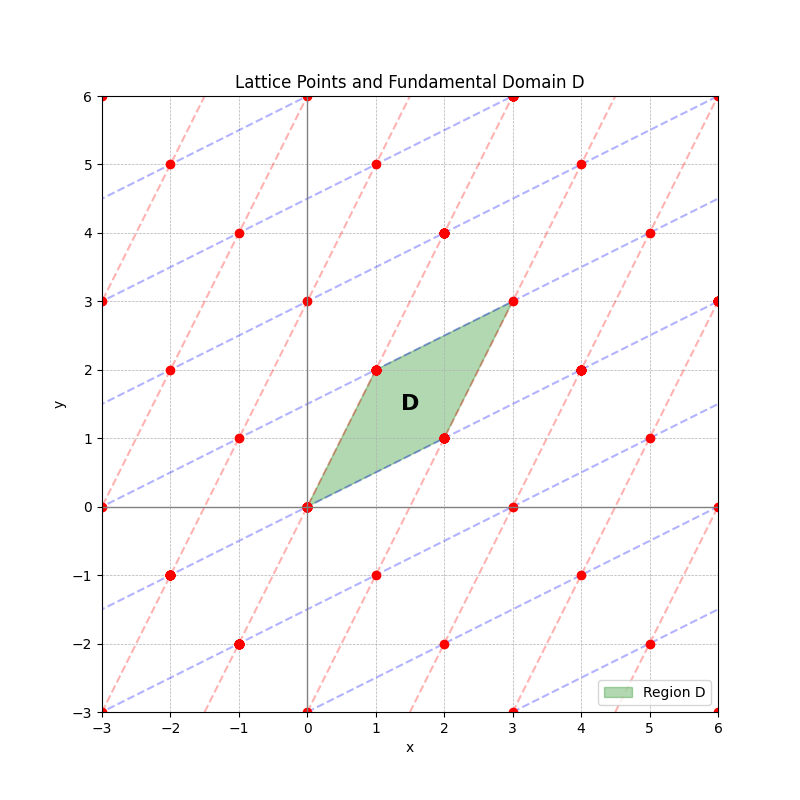
\includegraphics[width=\textwidth]{figures/Figure_1.png}
        \caption{Fundamental Domain \(D\)}
        \label{fig:first}
    \end{subfigure}
    \begin{subfigure}[b]{0.45\textwidth}
        \centering
        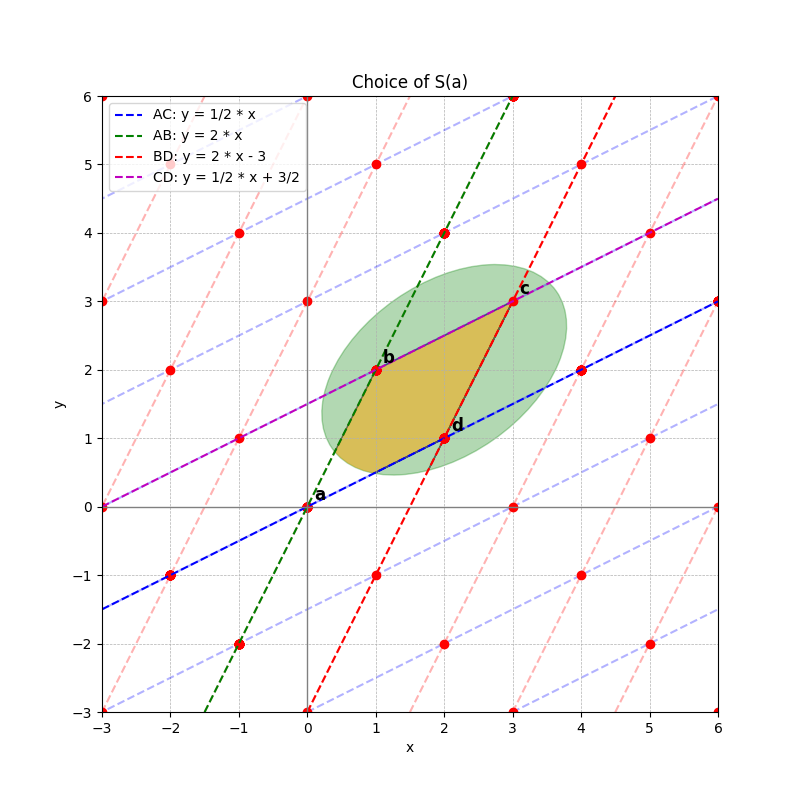
\includegraphics[width=\textwidth]{figures/Figure_2.png}
        \caption{Example of \(S(\mathbf{a})\): Yellow Area}
        \label{fig:second}
    \end{subfigure}
    \caption{\(\mathbb{R}^2\) Example}
    \label{fig:parallel_images}
\end{figure}

For all $\mathbf{v}\in \mathbb{R}^{n}$, $\mathbf{v}$ is uniquely expressed as $\mathbf{v}=\mathbf{u}+\mathbf{w}$ where $\mathbf{u}\in L$ and $\mathbf{w}\in D$. Define the volume of $L$ by $vol(L):=vol(D)=\left| \det(\mathbf{v}_{1},\dots,\mathbf{v}_{n})\right|$. 



\begin{proposition}
    Let $L$ be a lattice in $\mathbb{R}^{n}$, $S\subseteq \mathbb{R}^{n}$ be a bounded and measurable set such that $vol(S)\geq vol(L)$. Then $\exists \mathbf{x}, \mathbf{y}\in S$ such that $\mathbf{x}\neq \mathbf{y}$ and $\mathbf{x}-\mathbf{y}\in L$. 
\end{proposition}

\begin{proof}
    For all $\mathbf{a}\in L$, let $S(\mathbf{a})=(S-\mathbf{a})\cap D$. Then $S=\coprod\limits_{\mathbf{a}\in L}S(\mathbf{a})+\mathbf{a}$. Since 
    \[
    vol(S)=\sum_{\mathbf{a}\in L}vol(S(\mathbf{a}))\geq vol(L),
    \]
    there must be some $\mathbf{a}\neq \mathbf{b}\in L$ such that $S(\mathbf{a})\cap S(\mathbf{b})\neq \varnothing$. We may find $\mathbf{x}=\mathbf{v}+\mathbf{a}$, $\mathbf{y}=\mathbf{v}+\mathbf{b}\in S$, so $\mathbf{x}-\mathbf{y}=\mathbf{a}-\mathbf{b}\in L$. 
\end{proof}

\begin{theorem}[Minkowski's Convex Body]\label{thm-convexBody}
    Let $L$ be a lattice in $\mathbb{R}^{n}$. $S\subseteq \mathbb{R}^{n}$ be a bounded, measurable, convex ($\forall \mathbf{x},\mathbf{y}\in S$ and $\forall 0\leq t\leq 1$, the linear combination $t\mathbf{x}+(1-t)\mathbf{y}\in S$) and symmetric ($\mathbf{x}\in S\Rightarrow -\mathbf{x}\in S$). Suppose $vol(S)>2^{n}vol(L)$, then there exists a nonzero $\mathbf{v}\in S\cap L$. 
\end{theorem}

\begin{proof}
    Consider $vol(\frac{1}{2}S)=\frac{1}{2^{n}}vol(S)$. Then by above proposition, there exists $\mathbf{x},\mathbf{y}\in \frac{1}{2}S$ such that $\mathbf{x}-\mathbf{y}\in L$. Since $S$ is symmetric, $2\mathbf{x},-2\mathbf{y}\in S$. By the convexity of $S$, $\frac{1}{2}(2\mathbf{x})+\frac{1}{2}(-2\mathbf{y})\in S$. 
\end{proof}

\begin{remark}
    If $S$ is closed, then one can replace $vol(S)>2^{n}vol(L)$ by $vol(S)\geq 2^{n}vol(L)$. To see so, apply the theorem to $(1+\frac{1}{n})S$. Then there exist $\mathbf{v}_{n}\in (1+\frac{1}{n})S\cap L$. Since 
    \[
    \bigcap_{n=1}^{\infty}(1+\frac{1}{n})S=S
    \] 
    and 
    \[
    S\subseteq \cdots\subseteq (1+\frac{1}{n})S\subseteq 2S, 
    \]
    the sequence $(\mathbf{v}_{n})$ has a subsequence convergent to some $\mathbf{v}\in S$. 
\end{remark}

\begin{example}
    Let $p=1 \mod 4$ be a rational prime, then $\exists x,y\in \mathbb{Z}$ s.t. $x^{2}+y^{2}=p$. 
    \begin{proof}
        Let $s\in \mathbb{Z}_{p}^{*}$ be an element of order 4, such element exists since $\mathbb{Z}_{p}^{*}$ is an cyclic group of order $p-1$. Then $s^{2}=-1 \mod p$. 

        For $x,y \in \mathbb{Z}$ such that $x^{2}+y^{2}=0 \mod p$, then $(x+sy)(x-sy)=0\mod p$, i.e. $x=\pm sy\mod p$. By switching $s\to -s$ if necessary, we may assume $x=sy\mod p$. So $x=sy+zp$ for some $z\in \mathbb{Z}$. We may write 
        \[
        (x,y)=(sy+zp,y)=(s,1)y+(p,0)z. 
        \]
        We only need to find such $(x,y)$. 
        Consider the lattice $L=\langle (s,1),(p,0)\rangle_{\mathbb{Z}}$, then $vol(L)=p$. Let $S=\{(x,y)|x^{2}+y^{2}<2p\}$, then $vol(S)=2\pi p>2^{2}vol(L)$. By Theorem \ref{thm-convexBody}, there exists $(x,y)\in S\cap L$, i.e. $x^{2}+y^{2}<2p$ and $x=sy\mod p$. The only possible case is $x^{2}+y^{2}=p$. 
    \end{proof}
\end{example}

\section{Minkowski's Bound}
In this section, we will find a lattice and a bounded, measurable, convex and symmetric set and we will use Theorem \ref{thm-convexBody} to prove Theorem \ref{thm-MinkowskiBound}. 

Let $K:\mathbb{Q}$ be a number field with $[K:\mathbb{Q}]=n=r+2s$, where 
\[
\sigma_{1},\dots, \sigma_{r}:K\hookrightarrow\mathbb{R} \quad\text{real embeddings}
\]
\[
\left.\begin{aligned}
    \sigma_{r+1},\dots, \sigma_{r+s}\\
    \overline{\sigma_{r+1}},\dots, \overline{\sigma_{r+s}}
\end{aligned}\right\}:K\hookrightarrow \mathbb{C}\quad \text{complex embeddings}
\]

\begin{example}
    \begin{enumerate}
        \item Let $K=\mathbb{Q}(\sqrt{-5})$, then 
        \[
        \left.\begin{aligned}
            \sigma_{1}:a+b\sqrt{-5}\mapsto a+b\sqrt{-5}\\
            \sigma_{2}:a+b\sqrt{-5}\mapsto a-b\sqrt{-5}
        \end{aligned}\right\} \quad \text{are all complex embeddings}
        \]
        \item Let $K=\mathbb{Q}(\sqrt{3})$, then  
        \[
        \left.\begin{aligned}
            \sigma_{1}:a+b\sqrt{3}\mapsto a+b\sqrt{3}\\
            \sigma_{2}:a+b\sqrt{3}\mapsto a-b\sqrt{3}
        \end{aligned}\right\} \quad \text{are all real embeddings}
        \]
        \item Let $K=\mathbb{Q}(\sqrt[3]{2})$, then 
        \[
        \sigma_{1}:\sqrt[3]{2}\mapsto \sqrt[3]{2}\quad \text{ is real embedding}
        \]
        \[
        \left.\begin{aligned}
            \sigma_{2}:\sqrt[3]{2}\mapsto \sqrt[3]{2}\omega\\
            \overline{\sigma_{2}}:\sqrt[3]{2}\mapsto \sqrt[3]{2}\omega^{2}
        \end{aligned}\right\} \quad \text{are complex embeddings}
        \]
    \end{enumerate}
\end{example}

Define $\sigma:K\to \mathbb{R}^{r}\times \mathbb{C}^{s}\cong \mathbb{R}^{n}$ given by 
\[
\sigma: k\mapsto \begin{pmatrix}
    \sigma_{1}(k)\\
    \vdots\\
    \sigma_{r}(k)\\
    \mathrm{Re}(\sigma_{r+1}(k))\\
    \mathrm{Im}(\sigma_{r+1}(k))\\
    \vdots\\
    \mathrm{Re}(\sigma_{r+s}(k))\\
    \mathrm{Im}(\sigma_{r+s}(k))\\
\end{pmatrix}
\]

\begin{remark}
    Let $\{k_{1},\dots, k_{n}\}\subseteq K$ be a $\mathbb{Q}$-basis of $K$ (e.g. integral basis $\{\omega_{1},\dots,\omega_{n}\}$ of $\mathcal{O}_{K}$). Then 
    \[
    \begin{aligned}
        \det\begin{pmatrix} \uparrow & & \uparrow\\ \sigma(k_{1}) & \dots & \sigma(k_{n}) \\
        \downarrow & & \downarrow \end{pmatrix}&=\det\begin{pmatrix}
            \sigma_{1}(k_{1}) & &&  &\sigma_{1}(k_{n}) \\
            \vdots &&&&\vdots \\
            \sigma_{r}(k_{1})&&&&\sigma_{r}(k_{n})\\
            \mathrm{Re}(\sigma_{r+1}(k_{1}))&&&&\mathrm{Re}(\sigma_{r+1}(k_{n}))\\
            \mathrm{Im}(\sigma_{r+1}(k_{1}))&&\cdots&&\mathrm{Im}(\sigma_{r+1}(k_{n}))\\
            \vdots&&&&\vdots\\
            \mathrm{Re}(\sigma_{r+s}(k_{1}))&&&&\mathrm{Re}(\sigma_{r+s}(k_{n}))\\
            \mathrm{Im}(\sigma_{r+s}(k_{1}))&&&&\mathrm{Im}(\sigma_{r+s}(k_{n}))\\
        \end{pmatrix}\\
        &=\frac{1}{(2i)^{s}}\det \begin{pmatrix}
            \sigma_{1}(k_{1})& &&&\sigma_{1}(k_{n})\\
            \vdots &&&&\vdots \\
            \sigma_{r}(k_{1})&&& &\sigma_{r}(k_{n})\\
            \sigma_{r+1}(k_{1})& &\cdots& &\sigma_{r+1}(k_{n})\\
            \overline{\sigma_{r+1}}(k_{1})&&&&\overline{\sigma_{r+1}}(k_{n})\\
            \vdots&&&&\vdots\\
            \overline{\sigma_{r+s}}(k_{1})&&&&\overline{\sigma_{r+s}}(k_{n})
        \end{pmatrix}
    \end{aligned}
    \]
    (the last equality comes from simple elementary row operation $\begin{pmatrix}
        x \\ y
    \end{pmatrix} \to \begin{pmatrix}
        x+yi \\ x-yi
    \end{pmatrix}$). 
    In particular, 
    \[\det\begin{pmatrix} \uparrow & & \uparrow\\ \sigma(\omega_{1}) & \dots & \sigma(\omega_{n}) \\
        \downarrow & & \downarrow \end{pmatrix}=\frac{1}{(2i)^{s}}\det(\sigma_{i}(\omega_{j}))=\frac{1}{(2i)^{s}}\Delta(\underline{\omega})=\frac{1}{(2i)^{s}}\sqrt{\Delta^{2}(K)}.\]
\end{remark}

Now we consider $I\lhd \mathcal{O}_{K}$ a nonzero ideal. Note that $[\mathcal{O}_{K}:I]=N()I<\infty$. $\mathcal{O}_{K}=\langle \omega_{1},\dots, \omega_{n}\rangle_{\mathbb{Z}}$ where $\omega_{1},\dots,\omega_{n}$ is the integral basis (also a $\mathbb{Q}$-basis of $K$). Then $\mathcal{O}_{K}$ forms a lattice generated by $\{\sigma(\omega_{1}),\dots,\sigma(\omega_{n})\}$. 

$I$ is a sublattice of finite index so $I=\langle k_{1},\dots,k_{n}\rangle_{\mathbb{Z}}$, where $\{k_{1},\dots,k_{n}\}$ is also a $\mathbb{Q}$-basis of $K$. Denote the sublattice correspond to $I$ by $L_{I}$, which is generated by $\{\sigma(k_{1}),\dots, \sigma(k_{n})\}$. By the previous remark, 
\[
\begin{aligned}
    vol(L_{I})&=\left| \det(\sigma(k_{1}),\dots, \sigma(k_{n})) \right|=\frac{1}{2^{s}}\sqrt{\left| \Delta^{2}(k_{1},\dots, k_{n}) \right| }\\
    &=\frac{1}{2^{s}}\sqrt{[\mathcal{O}_{K}:I]^{2}\left| \Delta^{2}(K) \right| }=\frac{N(I)}{2^{s}}\sqrt{\left| \Delta^{2}(K) \right| }. 
\end{aligned}
\]
This $L_{I}$ will serve as the lattice.

For $t>0$, define set 
\[R_{t}=\{\begin{pmatrix}
    x_{1}\\
    \vdots\\
    x_{r}\\
    z_{r+1}\\
    \vdots\\
    z_{r+s}
\end{pmatrix}\in\mathbb{R}^{r}\times \mathbb{C}^{s}\cong \mathbb{R}^{n}|\sum_{i=1}^{r}\left| x_{i} \right| +\sum_{j=1}^{s}2\left| z_{r+j} \right| \leq t\}. \]
Then clearly $R_{t}$ is compact, convex and symmetric, whose volume is
\(
vol(R_{t})=\frac{2^{r}t^{n}(\frac{\pi}{2})^{s}}{n!}.
\)

\begin{theorem}\label{thm-MinkowskiBound}
    Let $I\lhd \mathcal{O}_{K}$, then $\exists \alpha\in I\backslash \{0\}$ such that 
    \[
    \left| Norm_{K /\mathbb{Q}} (\alpha)\right| \leq m_{K}N(I),
    \]
    where $m_{K}=(\frac{4}{\pi})^{s}\frac{n!}{n^{n}}\sqrt{\left| \Delta^{2}(K) \right| }$. 
\end{theorem}

\begin{proof}
    Take $t>0$ such that $\frac{\pi^{s}t^{n}}{n!}=4^{s}\sqrt{\left| \Delta^{2}(K) \right| }N(I)$ and consider $R_{t}\subseteq \mathbb{R}^{n}$. 
    \[vol(R_{t})=\frac{2^{r}t^{n}(\frac{\pi}{2})^{s}}{n!}=2^{r+2s}vol(L_{I})=2^{n}vol(L_{I}).\]
    By Theorem \ref{thm-convexBody}, there exists $\alpha\in I\backslash \{0\}$ s.t. $\sigma(\alpha)\in R_{t}$, i.e. 
    \[
    \sum_{i=1}^{r}\left| \sigma_{i}(\alpha) \right| +\sum_{j=1}^{s}2\left| \sigma_{r+j}(\alpha) \right|\leq t. 
    \]
    So 
    \[
    \frac{1}{n}\left(\sum_{i=1}^{r}\left| \sigma_{i}(\alpha) \right| +\sum_{j=1}^{s}(\left| \sigma_{r+j}(\alpha) \right|+\left| \overline{\sigma_{r+j}}(\alpha)\right|)\right) \leq \frac{t}{n},
    \]
    by AM-GM inequality, 
    \[\sqrt[n]{\prod_{\sigma\in \mathrm{Hom}(K,\mathbb{C})}\left| \sigma(\alpha) \right| }\leq \frac{t}{n}. \]
    Hence 
    \[
    \left| Norm_{K /\mathbb{Q}}(\alpha)\right|\leq (\frac{t}{n})^{n}=(\frac{4}{\pi})^{s}\frac{n!}{n^{n}}\sqrt{\left| \Delta^{2}(K) \right| }N(I). 
    \]
\end{proof}

\begin{corollary}
    Let $[K:\mathbb{Q}]=n$ be a number field. For any $c\in C_{K}=\{[I]|I\lhd\mathcal{O}_{K}\text{ nonzero}\}$, there exists $J\lhd \mathcal{O}_{K}$ such that $c=[J]$ and $N(J)\leq m_{K}$. 
\end{corollary}

\begin{proof}
    Fix $c\in C_{K}$ and consider $I\lhd \mathcal{O}_{K}$ such that $[I]=c^{-1}$. By Theorem \ref{thm-MinkowskiBound}, there exists $\alpha\in I\backslash \{0\}$ such that $\left| Norm_{K /\mathbb{Q}}(\alpha) \right| \leq m_{K}N(I)$. Note that 
    \begin{center}
    $(\alpha)\subseteq I$\quad  $\Rightarrow$ \quad $I\mid (\alpha)$\quad  $\Rightarrow$ \quad  there exists $J\lhd \mathcal{O}_{K}$ such that $IJ=(\alpha)$.    
    \end{center}
    So 
    \[
    N(I)N(J)=N(IJ)=N((\alpha)) = Norm_{K /\mathbb{Q}}(\alpha)\leq m_{K}N(I)
    \] 
    which gives $N(J)\leq m_{K}$. Moreover, since $IJ = (\alpha)$, $[I]*[J] = [(\alpha)] = e$ and hence $[J]=[I]^{-1}=c$. So the result follows.
\end{proof}

As an immediate consequence of the above corollary, one has $C_{K}=\{[J]\ |\ N(J) \leq m_{K}\}$. In other words, we can list all elements in $C_{K}$ by finding all ideals $J$ of norm less than or equal to $m_K$.

\section{Calculating Class Groups}
\begin{example}
    Let $K=\mathbb{Q}(\sqrt{-5})$, $\mathcal{O}_{K}=\mathbb{Z}[\sqrt{-5}]$. Then $r=0$ and $s=1$, $\left| \Delta^{2}(K) \right| =20$, so $m_{K}=\frac{4\sqrt{5}}{\pi} \approx 2.\cdots$. So 
    $$C_{K}=\{[J]\ |\ N(J)\leq 2\}.$$ 

    So we only have to study ideals with $N(J) = 1$ or $2$. In the case $N(J)=1$, $J=\mathcal{O}_{K}$ and hence $[J] = e$ is the identity element in $C_K$. As for $N(J)=2$, $[\mathcal{O}_{K}:J]=2$, so $J\lhd \mathcal{O}_{K}$ must be a prime ideal lying above 2. By Theorem \ref{thm-factorizationOfRationalPrimes}, the only possibility is the non-principal ideal $J=(2,1+\sqrt{-5})$. 
    Therefore, 
    $$C_K = \{e:=[\mathcal{O}_K],\ \  \tau:=[(2,1+\sqrt{-5})]\}$$ 
    has only two elements, i.e. $C_{K}\cong \mathbb{Z}_{2}$. Alternatively, one can check directly that
    $\tau^{2}=[(2,1+ \sqrt{-5})^2] = [(2)] =e$. 
\end{example}

\begin{example}
    Let \(K = \mathbb{Q}(\sqrt{-6}), \mathcal{O}_K = \mathbb{Z}[\sqrt{-6}] \). One can compute \(m_K = \frac{2}{\pi}\sqrt{24} \approx 3.\cdots\). Therefore
    \begin{align*}
        C_K = \left\{[J]\ |\  N(J)= 1,2,3\right\}
    \end{align*}
    Note that
    \begin{align*}
        N(J_1) = 1 &\Leftrightarrow J_1 = \mathcal{O}_K\\
        N(J_2) = 2 &\Leftrightarrow J_2 \triangleleft \mathcal{O}_K \text{ is a maximal ideal above }2. \text{ Since } (2) = (2,\sqrt{-6})^2, \text{ this implies } J_2 = (2,\sqrt{-6})\\
        N(J_3) = 3 &\Leftrightarrow J_3 = (3,\sqrt{-6}).
    \end{align*}
    Therefore, \[C_K = \left\{e=[O_K], [J_2], [J_3]\right\}.\] 
    We can easily check that \([J_2] \neq e\) is not principal, otherwise suppose \(J_2 = (a+b\sqrt{-6})\) for some \(a,b \in \mathbb{Z}\), \(N(J_2)= a^2+6b^2 = 2\). The only choice for \(b\) is \(b = 0\), implies  \(a^2 =2\), \(a \notin \mathbb{Z}\) contradiction. Similarly one has \([J_3] \neq e\). Also, note that 
    \[[J_2]^2 = [(2)], \quad [J_3]^2 = [(3)]  \quad \quad \Rightarrow \quad \quad [J_2]^2 = [J_3]^2 = e.\]
    which implies \(C_K\) has no elements of order 3. Thus \(C_K \ncong \mathbb{Z}_3\), implying that $[J_2] = [J_3]$ and 
    \[C_K = \{e, [J_2] = [J_3]\} \cong \mathbb{Z}_2.\]

    Alternatively, one can also check directly that $[J_2] = [J_3]$: since \(\sqrt{-6} = 3\sqrt{-6} + \sqrt{-6}(-2)\) we have
    \begin{align*}
        \sqrt{-6} \in J_3 J_2 \quad \Rightarrow \quad (\sqrt{-6}) \subseteq J_3 J_2\quad \Rightarrow \quad J_3 J_2 | (\sqrt{-6})
    \end{align*}
    By computing norm \(N(J_2) N(J_3) = 2 \times 3 = 6 = N\left((\sqrt{-6})\right)\), we can conclude that 
    \begin{align*}
        J_3J_2 = (\sqrt{-6}) \quad \Rightarrow \quad [J_3]*[J_2] = [(\sqrt{6})] = e \quad \Rightarrow \quad [J_3] = [J_2]^{-1} = [J_2]
    \end{align*}
    since $[J_2]^2 = e$.
\end{example}

\begin{remark} \label{rmk-ckgenerator}
    By Minikowski Bound, we can easily have \begin{align*}
        C_K = \left\{[J]| N(J) \leq m_k\right\}.
    \end{align*}
    If we only care about the generators of \(C_K\) (as a finite abelian group), we only need to study \(J\) with \(N(J) = P\) for \(p \leq m_k\) rational prime, i.e.
    $$C_K = \langle J\ |\ N(J) = p,\ p \leq m_K\ \text{rational prime}\rangle.$$
    For instance, suppose \(N(J) = 6\). Then for all \(\alpha \in \mathcal{O}_K, 6\alpha \in J\) (since \(N(J) = |\mathcal{O}_K/J|=6\)). We have
    \begin{align*}
        (6) \subseteq J \quad \Rightarrow \quad J|(6)\quad \Rightarrow \quad J|(2)(3).
    \end{align*}
    By Dedekind's theorem, \(J\) can be factorized into (some prime ideals lying above 2) \(\times\) (some prime ideals lying above 3). In other words, the prime ideals lying above $2$ and $3$ generates \(J\).
\end{remark}

\begin{example}
    Let \(K = \mathbb{Q}(\sqrt{-163})\) and \(\mathcal{O}_K = \displaystyle \mathbb{Z}[\frac{1+\sqrt{-163}}{2}]\). One can easily compute \(m_k = \frac{4}{\pi} \frac{1}{2} \sqrt{163} = 8. \cdots\).

    By the Remark above, 
    \[C_K = \langle J\ |\ N(J) = 2,3,5,7 \rangle\] 
    So we can apply theorem \ref{thm-factorizationOfRationalPrimes}, with \(\alpha = \frac{1+\sqrt{-163}}{2}\) to find the ideals $J$ lying above $2,3,5,7$. Since the minimal polynomial of $\alpha$ is
    \begin{align*}
        m_\alpha(x) = x^2 - x + 41,
    \end{align*}
    we can check that 
    \begin{itemize}
        \item[\((2)\):] \(\bar m_\alpha(x) = x^2 + x + 1\) irreducible in \(\mathbb{Z}_2[x] \Rightarrow (2)\) is prime;
        \item[\((3)\):] \(\bar m_\alpha(x) = x^2 + x - 1\) irreducible in \(\mathbb{Z}_3[x] \Rightarrow (3)\) is prime;
        \item[\((5)\):] \(\bar m_\alpha(x) = x^2 + x + 1\) irreducible in \(\mathbb{Z}_5[x] \Rightarrow (5)\) is prime;
        \item[\((7)\):] \(\bar m_\alpha(x) = x^2 + x - 1\) irreducible in \(\mathbb{Z}_7[x] \Rightarrow (7)\) is prime.
    \end{itemize}
    Therefore there is no \(J\) with \(N(J) =2,3,5,7\). Hence 
    \begin{align*}
        C_K = <\emptyset> = {e}
    \end{align*}
    is the trivial group. \(i.e.\) \(\mathcal{O}_K\) is a PID.
\end{example}

\begin{example}
    Let \(K = \mathbb{Q}(\sqrt{-29})\) and \(\mathcal{O}_K = \displaystyle \mathbb{Z}[-29]\). One can easily compute \(m_k = \frac{2}{\pi} \sqrt{116} = 6. \cdots\). So we need to study \(J \triangleleft \mathcal{O}_K\) with \(N(J) = 2,3,5\), where
    \begin{align*}
        (2) &=  P^2 = (2,1+\sqrt{-29})^2;\\
        (3) &= Q Q' = (3, 1+\sqrt{-29})(3,1-\sqrt{-29});\\
        (5) &= R R' = (5, 1+\sqrt{-29})(5, 1-\sqrt{-29}).
    \end{align*}
    we can get \(C_K = \left< [P], [Q], [Q'], [R], [R']  \right>\). We want to study the relation between ideal classes \([P],[Q],[R], [Q'],[R']\). Obviously we have 
    \begin{align*}
        [P]^2 = [Q][Q'] = [R][R'] = e\\
        [Q'] = [Q]^{-1} = [Q]^a\\
        [R'] = [R]^{-1} = [R]^b
    \end{align*}
    for some \(a,b > 1\) (otherwise $Q' = Q$ or $R' = R$, contradicting the unique factorization in Theorem \ref{thm-factorizationOfRationalPrimes}). We can simplify \(C_K = \left< [P], [Q], [R]\right>\), where \([P]\) have order 2 and \([Q]\) and $[R]$ has order greater or equal to \(3\).
    
    To look at the orders of $[Q]$ and $[R]$, one needs to do some trial and error. By observation, $\mathrm{Norm}_{K/\mathbb{Q}}(3+2\sqrt{-29}) = 3^2 + 4\cdot 29 = 125 = 5^3$, so we study the prinicpal ideal
    \(I = (3+2 \sqrt{-29})\). 

    By the argument given in Remark \ref{rmk-ckgenerator}, 
    $$I\ |\ (125) = (5)^3 = R^3(R')^3,$$
    thus there are 4 possible ways in prime factorization as follows
    \begin{align*}
        I = R^3, R^2 R' , R (R')^2 , (R')^3.
    \end{align*}
    Suppose \(R|I\), implying that \(I \subseteq R\), we have
    \begin{align*}
        3+2\sqrt{-29} \in I \subseteq R,\quad \quad 2 (1+\sqrt{-29}) \in R,\\ 
    \end{align*}
    Therefore, 
    \begin{align*}
        \left\{(3+2\sqrt{-29}) - 2(1+\sqrt{-29}) \right\} \in R\quad 
        \Rightarrow \quad 1\in R\quad
        \Rightarrow \quad R= \mathcal{O}_K,
    \end{align*}
    which is a contradiction. Therefore the only choice for prime factorization is \(I = (R')^3\), and we can compute
\begin{align*}
    [R']^3 = [I] =e \quad 
    \Rightarrow\quad  \left([R]^{-1}\right)^3 = e\quad
    \Rightarrow \quad [R]^3 = e.
\end{align*}
We conclude that degree of \([R]\) is \(3\). 

\medskip
Now we study \(I' = (1+\sqrt{-29})\) with \(N(J) = 30\), one can easily check that \(I' | (2)(3)(5)\), which implies that 
\begin{align*}
    I' | P^2\cdot Q Q'  \cdot RR'.
\end{align*}
Since \(N(I') = 30 = 2\times3 \times 5\), therefore we have
\begin{align*}
    I = \left\{\begin{matrix}
PQR \\
PQ'R \\
PQR' \\
PQ'R'
\end{matrix}\right. \quad \Rightarrow \quad [I] = \left\{\begin{matrix}
[P][Q][R] \\
[P][Q]^{-1}[R] \\
[P][Q][R]^{-1} \\
[P][Q]^{-1}[R]^{-1}
\end{matrix}\right.
\end{align*}
hence \([Q]\) can be expressed as
\begin{align*}
    [Q] =  [P][R] \quad \text{or}\quad [P][R]^{-1} \in \left<[P] ,[R]\right>.
\end{align*}

As a conclusion, 
\[C_K = \langle [P],[R]\ |\ [P]^2 = e,\ [R]^3 = e \rangle \cong \mathbb{Z}_2 \times \mathbb{Z}_3 \cong \mathbb{Z}_6.\]
\end{example}


\section{Applications to Diophantine Equations}
We will end by presenting two examples on how the knowledge on $C_K$ helps solve certain Diophantine equations:
\begin{example}
Show that there are no integer solutions to $Y^2+37 = X^3$.
\end{example}
\begin{proof}
Let $K = \mathbb{Q}(\sqrt{37})$, with $\mathcal{O}_K = \mathbb{Z}[\sqrt{-37}]$. One can check that $C_K \cong \mathbb{Z}_2$. Then the equation can be factorized as:
$$\{Y + \sqrt{-37}\}\{Y - \sqrt{-37}\} = X^3$$
\noindent {\bf Claim 1. $2, 37 \nmid X$}. 

To see so, suppose on contrary that $2 \mid X$, then $X^3 = Y^2 + 37 \equiv 0 \mod 8$, which implies $Y^2 \equiv 3 \mod 8$. However, one can easily check that all square numbers can only have $n^2 \equiv 0, 1, 4 \mod8 $.

On the other hand, if $37 \mid X$, then obviously one also has $37 \mid Y$. Write $X = 37a$ and $Y = 37b$, then
$$(37b)^2 + 37 = (37a)^3 \quad \Rightarrow \quad 37b^2 + 1 = 37^2a^3 \equiv 0 \mod 37$$
But $37b^2 + 1 \equiv 1 \mod 37$, which again gives a contradiction. \qed

\medskip 
\noindent{\bf Claim 2. The principal ideals $(Y + \sqrt{-37})$ \& $(Y - \sqrt{-37})$ are coprime}. 

Suppose on contrary there exists a prime ideal $P \mid (Y + \sqrt{-37})$ and $ P \mid (Y - \sqrt{-37})$. Thus 
$$(Y \pm \sqrt{-37}) \subseteq P \quad \Rightarrow  \quad Y \pm \sqrt{-37} \in P  \quad \Rightarrow  \quad 2\sqrt{-37} = \{Y + \sqrt{-37}\} - \{Y - \sqrt{-37}\} \in P$$  
and hence
$$(2\sqrt{-37}) \subseteq P  \quad
\Rightarrow  \quad P \mid (2\sqrt{-37}) = (2)(\sqrt{-37})  \quad \Rightarrow  \quad P \mid (2) \text{ or } P \mid (\sqrt{-37})$$
Therefore, $P = (2, 1+ \sqrt{-37})$ or $(\sqrt{-37})$. 

Suppose $P = (2, 1+ \sqrt{-37})$, then 
\begin{align*}
(2) = P^2 | (Y+\sqrt{-37})(Y-\sqrt{-37}) = (Y^2+37) = (X^3) \quad &\Rightarrow \quad N((2)) \mid N((X^3)) \\
&\Rightarrow \quad  4 \mid X^6 \\ &\Rightarrow \quad 2 \mid X,\end{align*}
contradicting Claim 1.

On the other hand, suppose $P = (\sqrt{-37})$, then
\begin{align*}
Y + \sqrt{-37} \in (\sqrt{-37}) \ &\Rightarrow \ Y = \{Y + \sqrt{-37}\} - \sqrt{-37} \in (\sqrt{-37}) \\ &\Rightarrow \ (\sqrt{37}) \mid (Y) \\
&\Rightarrow \  37 = N((\sqrt{37})) \mid N((Y)) = Y^2 
\end{align*}
Hence $37 \mid Y$, and the original equation implies that $37 \mid X$, contradicting Claim 1 again.  \qed

\bigskip
Consider the ideal factorization
$$(Y + \sqrt{-37})(Y - \sqrt{-37}) = (X)^3 = P_1^{3e_1} P_2^{3e_2} \cdots P_r^{3e_r}$$ 
where $(X) = P_1^{e_1} P_2^{e_2}\dots P_r^{e_r}$ is the prime ideal factorization of $(X)$. By Claim 2 and Dedekind's Theorem, if the prime ideal $P_i \mid (Y+\sqrt{-37})$, then
$P_i \nmid (Y-\sqrt{-37})$ and hence $P_i^{3e_i} \nmid (Y+\sqrt{-37})$. Therefore,
$$(Y + \sqrt{-37}) = I^3  \quad \quad (*)$$ 
where $I = P_{i_1}^{e_{i_1}}\dots P_{i_l}^{e_{i_l}}$.

Now study ideal class group:
$$e = [(Y + \sqrt{-37})] = [I]^3$$
Since $|C_K| = 2$, $[I]^2 = e$ and hence $[I]^3 = [I]$, which gives
$$e = [(Y + \sqrt{-37})] = [I],$$
i.e. $I = (a+b\sqrt{-37})$ itself is a principal ideal. Hence $(*)$ gives
\begin{align*}
(Y + \sqrt{-37}) &= (a+b\sqrt{-37})^3 = (\{a^3-111ab^2\} + \{3a^2b-37\}\sqrt{-37}) \\ 
\Rightarrow \quad Y + \sqrt{-37} &= \pm\{\{a^3-111ab^2\} + \{3a^2b-37b^3\}\sqrt{-37}\}
\end{align*}

Since $\{1,\sqrt{-37}\}$ is a $\mathbb{Q}$-basis of $K$, they are linearly independent and hence
$$Y = \pm a(a^2-111b^2), \quad \quad  1 = \pm b(3a^2-37b^2).$$
But the second equation implies that $b = \pm 1$ and hence
$3a^2 - 37 = \pm 1$, which implies 
$3a^2 = 38$ or $36$. But this is impossible.

\medskip
Consequently, the original equation $Y^2+37 = X^3$ has no integer solutions.
\end{proof}



\begin{example}
We have seen that for $K = \mathbb{Q}(\sqrt{6})$ and $\mathcal{O}_K = \mathbb{Z}[\sqrt{6}]$, $C_K \cong \mathbb{Z}_2$. We will use it to find solutions of the equation:
\[
Y^2 + 54 = X^3 \quad \text{(*)}
\]
\end{example}
\begin{proof} {\bf Claim 1: $2, 3 \nmid y$.}

Suppose on contrary $2 \mid Y$, then obviously $2 \mid X$ and hence $8 \mid X^3 = Y^2 + 54$. But $Y^2+54 \equiv 2 \mod 4$. 

Now suppose $3 \mid Y$. Then $3 | X$. Write $Y = 3a$ and $X = 3b$, one has
$$9a^2 + 54 = 27b^3 \quad \Rightarrow \quad a^2 + 6 = 3b^3$$
which forces $3 \mid a \Rightarrow a =3c$ for some integer $c$. Thus
$$(3c)^2 + 6 = 3b^3 \quad \Rightarrow\quad 3c^2 + 2 = b^3.$$
But $b^3 \equiv 0,1,8 \mod 9$, while $3c^2 + 2 \equiv 2, 5 \mod 9$.  \qed

\medskip
\noindent {\bf Claim 2:
$(Y + 3\sqrt{6}), (Y - 3\sqrt{6})$ has no common prime factors.}

Suppose on contrary $P \mid (Y \pm 3\sqrt{6})$, then as before
$$2 \cdot 3\sqrt{6} \in P \ \Rightarrow\ P \mid (6\sqrt{6}) = (\sqrt{6})^3 \ \Rightarrow \ P \mid (\sqrt{6})\ \Rightarrow \ (\sqrt{6}) \subseteq P \ \Rightarrow \ \sqrt{6} \in P$$
Thus
$$\sqrt{6}, Y + 3\sqrt{6} \in P\ \Rightarrow\ Y \in P \ \Rightarrow \  P \mid (Y)\ \Rightarrow\ N(P) \mid N((Y)) = Y^2$$
But $P \mid  (\sqrt{6})$ implies that $N(P) \mid N((\sqrt{6})) = 6$ and hence $2,3 \mid Y^2$, contradicting Claim 1. \qed


\bigskip
As in Example 1, one can use Claim 2 and the fact that $|C_K| =2$ to conclude that 
$$(Y + 3\sqrt{6}) = (a + b \sqrt{-6})^3 = (\{a^3-18ab^2\} + \{3a^2b-6b^3\}\sqrt{-6})$$
for some $a,b \in \mathbb{Z}$, which yields
$$Y = \pm a(a^2-18b^2) \quad \quad 3 = \pm 3b(a^2-2b^2)$$
So $b = \pm 1$ and $a = 1$ from the second equation, forcing $Y = \pm 17$ in the first equation. Putting it back to the original equation, one has $X = 7$.

\medskip
In conclusion, the only solutions of the Diophantine equation are
\[
(X,Y) = (7, \pm 17).
\]
\end{proof}



\end{document}

